%definira klasu dokumenta 
\documentclass[12pt]{report} 

%prostor izmedu naredbi \documentclass i \begin{document} se zove uvod. U njemu se nalaze naredbe koje se odnose na cijeli dokument

%osnovni LaTex ne može riješiti sve probleme, pa se koriste različiti paketi koji olakšavaju izradu željenog dokumenta
\usepackage[croatian]{babel} 
\usepackage{amssymb}
\usepackage{amsmath}
\usepackage{txfonts}
\usepackage{mathdots}
\usepackage{titlesec}
\usepackage{array}
\usepackage{lastpage}
\usepackage{etoolbox}
\usepackage{tabularray}
\usepackage{color, colortbl}
\usepackage{adjustbox}
\usepackage{geometry}
\usepackage[classicReIm]{kpfonts}
\usepackage{hyperref}
\usepackage{fancyhdr}

\usepackage{float}
\usepackage{setspace}
\restylefloat{table}


\patchcmd{\chapter}{\thispagestyle{plain}}{\thispagestyle{fancy}}{}{} %redefiniranje stila stranice u paketu fancyhdr

%oblik naslova poglavlja
\titleformat{\chapter}{\normalfont\huge\bfseries}{\thechapter.}{20pt}{\Huge}
\titlespacing{\chapter}{0pt}{0pt}{40pt}


\linespread{1.3} %razmak između redaka

\geometry{a4paper, left=1in, top=1in,}  %oblik stranice

\hypersetup{ colorlinks, citecolor=black, filecolor=black, linkcolor=black,	urlcolor=black }   %izgled poveznice


%prored smanjen između redaka u nabrajanjima i popisima
\newenvironment{packed_enum}{
	\begin{enumerate}
		\setlength{\itemsep}{0pt}
		\setlength{\parskip}{0pt}
		\setlength{\parsep}{0pt}
	}{\end{enumerate}}

\newenvironment{packed_item}{
	\begin{itemize}
		\setlength{\itemsep}{0pt}
		\setlength{\parskip}{0pt}
		\setlength{\parsep}{0pt}
	}{\end{itemize}}




%boja za privatni i udaljeni kljuc u tablicama
\definecolor{LightBlue}{rgb}{0.9,0.9,1}
\definecolor{LightGreen}{rgb}{0.9,1,0.9}

%Promjena teksta za dugačke tablice
\DefTblrTemplate{contfoot-text}{normal}{Nastavljeno na idućoj stranici}
\SetTblrTemplate{contfoot-text}{normal}
\DefTblrTemplate{conthead-text}{normal}{(Nastavljeno)}
\SetTblrTemplate{conthead-text}{normal}
\DefTblrTemplate{middlehead,lasthead}{normal}{Nastavljeno od prethodne stranice}
\SetTblrTemplate{middlehead,lasthead}{normal}

%podesavanje zaglavlja i podnožja

\pagestyle{fancy}
\lhead{Programsko inženjerstvo}
\rhead{True Blood}
\lfoot{Illidimus Digitus}
\cfoot{stranica \thepage/\pageref{LastPage}}
\rfoot{\today}
\renewcommand{\headrulewidth}{0.2pt}
\renewcommand{\footrulewidth}{0.2pt}


\begin{document} 
	
	
	
	\begin{titlepage}
		\begin{center}
			\vspace*{\stretch{1.0}} %u kombinaciji s ostalim \vspace naredbama definira razmak između redaka teksta
			\LARGE Programsko inženjerstvo\\
			\large Ak. god. 2021./2022.\\
			
			\vspace*{\stretch{3.0}}
			
			\huge {True Blood}\\
			\Large Dokumentacija, Rev. \textit{2}\\
			
			\vspace*{\stretch{12.0}}
			\normalsize
			Grupa: \textit{Illidimus Digitus}\\
			Voditelj: \textit{David Kerman}\\
			
			
			\vspace*{\stretch{1.0}}
			Datum predaje: \textit{14.01.2022.}\\
	
			\vspace*{\stretch{4.0}}
			
			Nastavnik: \textit{Ivan Lovrić}\\
		
		\end{center}

	
	\end{titlepage}

	
	\tableofcontents
	
	
	\chapter{Dnevnik promjena dokumentacije}
		
		\begin{longtblr}[
				label=none
			]{
				width = \textwidth, 
				colspec={|X[2]|X[13]|X[3]|X[3]|}, 
				rowhead = 1
			}
			\hline
			\textbf{Rev.}	& \textbf{Opis promjene/dodatka} & \textbf{Autori} & \textbf{Datum}\\[3pt] \hline
			0.1 & Napravljen predložak.	& Kerman & 28.10.2021. 		\\[3pt] \hline 
			0.2	& Dodani funkcionalni zahtjevi & Kerman, Jurinić & 28.10.2021. 	\\[3pt] \hline 
			0.3 & Dodani opisi UC11 - UC19 & Kerman & 25.10.2021. \\[3pt] \hline 
			0.4 & Dodani opisi UC1 - UC10 & Jurinić & 29.10.2021 \\[3pt] \hline 
			0.5 & Sekvencijski dijagrami & Hudiček & 31.10.2021 \\[3pt] \hline 
			0.6 & Opis projektnog zadatka & Šlezak & 01.11.2021 \\[3pt] \hline 
			0.7 & Dodan opis baze & Vugrinec & 03.11.2021 \\[3pt] \hline 
			0.6 & Dodani dijagrami obrazaca uporabe & Kerman & 03.11.2021 \\[3pt] \hline 
			0.7 & Dodani nefunkcionalni zahtjevi & Okreša & 04.11.2021 \\[3pt] \hline 
			0.8 & Dodani opisi varijabli u opisu baze & Vugrinec & 05.11.2021 \\[3pt] \hline 
			0.9 & Definirana arhitektura sustava & Kerman & 10.11.2021. \\[3pt] \hline 
			0.10 & Osvježeni obrasci upotrebe & Kerman & 12.11.2021. \\[3pt] \hline 
			0.11 & Popravljen opis baze & Vugrinec & 15.11.2021. \\[3pt] \hline 
			0.12 & Popravljen pravopis & Kerman & 15.11.2021. \\[3pt] \hline 	
			0.13 & Popravljeni obrasci uporabe & Kerman, Jurinić & 17.11.2021. \\[3pt] \hline 			
			0.14 & Dodani opisi i dijagrami razreda & Kerman, Hudiček & 17.11.2021. \\[3pt] \hline 							
			\textbf{1.0} & Verzija samo s bitnim dijelovima za 1. ciklus & Kerman & 19.11.2021. \\[3pt] \hline 
			1.1 & Dodani opisi dijagrama (stanja, aktivnosti, komponenti, razmještaja) & Kerman & 12.12.2021. \\[3pt] \hline 
			1.2 & Dodani dijagrami (stanja, aktivnosti, komponenti, razmještaja) & Kerman & 13.12.2021. \\[3pt] \hline 
			1.3 & Popravljeni opisi obrazaca uporabe & Kerman & 28.12.2021. \\[3pt] \hline 
			1.4 & Popravljeni dijagrami obrazaca uporabe i aktivnosti & Kerman & 08.01.2022. \\[3pt] \hline 
			1.5 & Dodani unit testovi & Kerman & 10.01.2022. \\[3pt] \hline 
			1.6 & Dodane korištene tehnologije i alati i Zaključak & Kerman & 11.01.2022. \\[3pt]
			 \hline 
			1.7 & Dodani selenium testovi & Pardon & 12.01.2022. \\[3pt] \hline 
			1.8 & Popravljen dijagram baze & Vugrinec & 12.01.2022. \\[3pt] \hline 
			1.9 & Popravljeni nefunkcionalni zahtjevi & Okreša & 13.01.2022. \\[3pt] \hline 
			1.10 & Popravljeni obrasci uporabe & Jurinić & 13.01.2022. \\[3pt] \hline 
			1.11 & Popravljeni sekvenijski dijagram & Hudiček & 13.01.2022. \\[3pt] \hline 
			1.12 & Ažuriran dijagram razreda & Hudiček & 13.01.2022. \\[3pt] \hline 
			1.13 & Dodano poglavlje "Puštanje u pogon" & Šlezak & 13.01.2022. \\[3pt] \hline 
		\end{longtblr}
	
	
		
	\chapter{Opis projektnog zadatka}
		
		Cilj ovog projekta je razviti programsku podršku za stvaranje responzivne web aplikacije \textit{"True Blood"} koja omogućuje prikupljanje i objavljivanje podataka o prikupljenim dozama darivane krvi te općenito vođenje evidencije podataka za banke krvi.
		Ovaj projekt omogućio bi smanjenje vremena i znatno olakšanje obavljanje administracijskih poslova pri samoj djelatnosti prikupljanja krvi. Vođenje evidencije 'klasičnim' načinom u današnje vrijeme je skupo, sporo i neefikasno, a ovim projektom nestaje potreba za standardnom hrpom papira, što ujedno i smanjuje kompliciranost, potrebu za dodatnom radnom snagom te dodatne troškove, a da ne govorimo o mogućoj dodatnoj redundanciji podataka i njihovoj mogućoj većoj opsežnosti.\\
		
		Neregistriranom/neprijavljenom korisniku se na javim web stranicama prikazuje trenutno stanje zaliha različitih krvnih grupa te mogućnost logina i registracije. U sustavu postoje 3 vrste korisnika:
		\begin{packed_item}
			\item{administrator}
			\item{djelatnik banke}
			\item{donor}
		\end{packed_item}
		Djelatnik banke i donor na svoju email adresu dobivaju link za aktivaciju korisničkog računa,privremenu lozinku te djelatnici dobivaju svoje korisničko ime,a donor svoj donorId koji će koristiti kao korisničko ime. Prilikom aktivacije korisničkog računa korisnik odabire lozinku koju će koristiti.
		\underbar{ \textit{Administrator} }sustava administrira korisničke račune. On kreira nove korisničke račune za ulogu djelatnika banke te može u bilo kojem trenutku deaktivirati bilo koji korisnički račun. Administrator isto tako definira gornju i donju granicu optimalne količine krvi za svaku krvnu grupu, kako bi sustav dojavio upozorenja u slučaju prekoračenja gornje ili donje granice.
		\underbar{ \textit{Djelatnik banke} }krvi evidentira podatke o donoru kada potencijalni donor pristupa darivanju krvi. Ukoliko donor još nije evidentiran u sustavu, djelatnik banke kreira njegov korisnički profil te popunjava sve potrebne podatke:
		\begin{packed_item}
			\item{matični podaci}
			\item{kontakt podaci}
			\item{zdravstveni podaci}
		\end{packed_item}
		Ukoliko je donor već koristio usluge ustanove, povlače se zadnji aktualni podaci koje djelatnik banke po potrebi nadopunjuje. Djelatnik banke u sustav evidentira svaki pokušaj doniranja. Prije nego donor pristupi darivanju krvi, djelatnik banke provjerava njegovo zdrastveno stanje, te prema tome može prihvatiti te privremeno ili trajno odbiti donora.
		Djelatnik banke evidentira uspješno doniranje krvi, ali i potrošnju (tj. slanje određenog broja jedinica krvi van banke). Time se povećava tj. smanjuje zaliha određene krvne grupe što je odmah vidljivo na javim web stranicama, a ukoliko se prekorači gornja ili donja granica zalihe za neku krvnu grupu, djelatnici dobivaju notifikaciju putem emaila.
		\underbar{ \textit{Donori} }imaju mogućnost sami se registrirati na web stranici te ažurirati svoje matične i kontakt podatke te pregledavati zapisane zdrastvene podatke i povijest svojih (uspješnih i odbijenih) doniranja. Svakom evidencijom uspješnog darivanja krvi, donor na svoj email dobiva poruku s potvrdom o pristupanju darivanju krvi u PDF formatu koju može i sam podići naknadno iz aplikacije. Prilikom svakog logiranja donora u sustav (koji nema trajnu zabranu darivanja krvi), aplikacija će donoru prikazati poruku u ovisnosti o trenutnom stanju zaliha krvi za njegovu krvnu grupu:
		\begin{packed_item}
			\item{stanje zaliha je ispod optimalne granice}
			\item{stanje zaliha je optimalno}
			\item{stanje zaliha je iznad gornje optimalne granice}
		\end{packed_item}
		Donori dobivaju notifikacije od sustava nakon što istekne dopušteni period od zadnjeg darivanja i ukoliko zaliha njihove krvne grupe padne ispod minimalne granice.\\
		
		Ovo rješenje bi mogle koristiti jednako manje ali i veće banke krvi koje još nemaju informacijski sustav za prikupljanje i objavljivanje podataka o prikupljenim dozama krvi. Pošto se radi o web aplikaciji, ona se lako može implementirati u postojeći sustav web stranica koju pojedini potencijalni korisnik rješenja ima, te se, ukoliko je to zbilja potrebno, i stil same web aplikacije može prilagoditi da korespondira sa stilom postojećih web stranica. Isto tako, ukoliko potencijalni korisnik već posjeduje neku vlastitu bazu podataka koju koristi za neku funkcionalnost logiranja i/ili evidenciju nekih relativnih podataka te bi ju htio nastaviti koristiti, rješenje je moguće prilagoditi da se koristi zahtijevanim podacima.\\
		
		Trenutno u hrvatskoj postoje implementirani dijelovi ovih rješenja, točnije, postoje javne stranice gdje se prikazuje trenutno stanje zaliha različitih krvnih grupa (npr. slika \ref{fig:HZTMprimjer}). Ako pogledamo malo šire po svijetu, možemo uočiti da ima očito i nekih razrađenih sistema za evidenciju sa loginom donora (npr. slika \ref{fig:AmericanRedCrossPrimjer}), no sva ta rješenja nemaju kompaktno razrađen sustav kod kojih bi prijašnji donori dobivali notifikacije s obzirom na stanje banke krvi i pojedinačnih krvnih grupa, koje je javno i na jednostavan (grafički) način dostupno svima.
		\begin{figure}[H]
			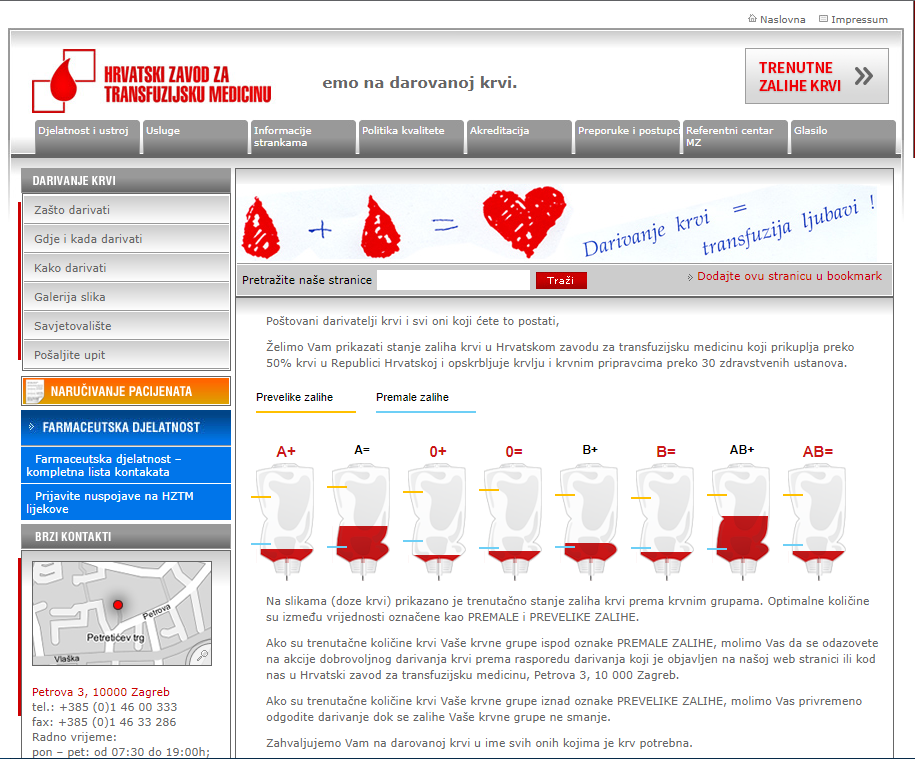
\includegraphics[scale=0.8]{slike/HZTMprimjer.PNG} %veličina slike u odnosu na originalnu datoteku i pozicija slike
			\centering
			\caption{Primjer javno dostupnih podataka o stanju banke krvi Hrvatskog zavoda za transfuzijsku medicinu}
			\label{fig:HZTMprimjer}
		\end{figure}
		\begin{figure}[H]
			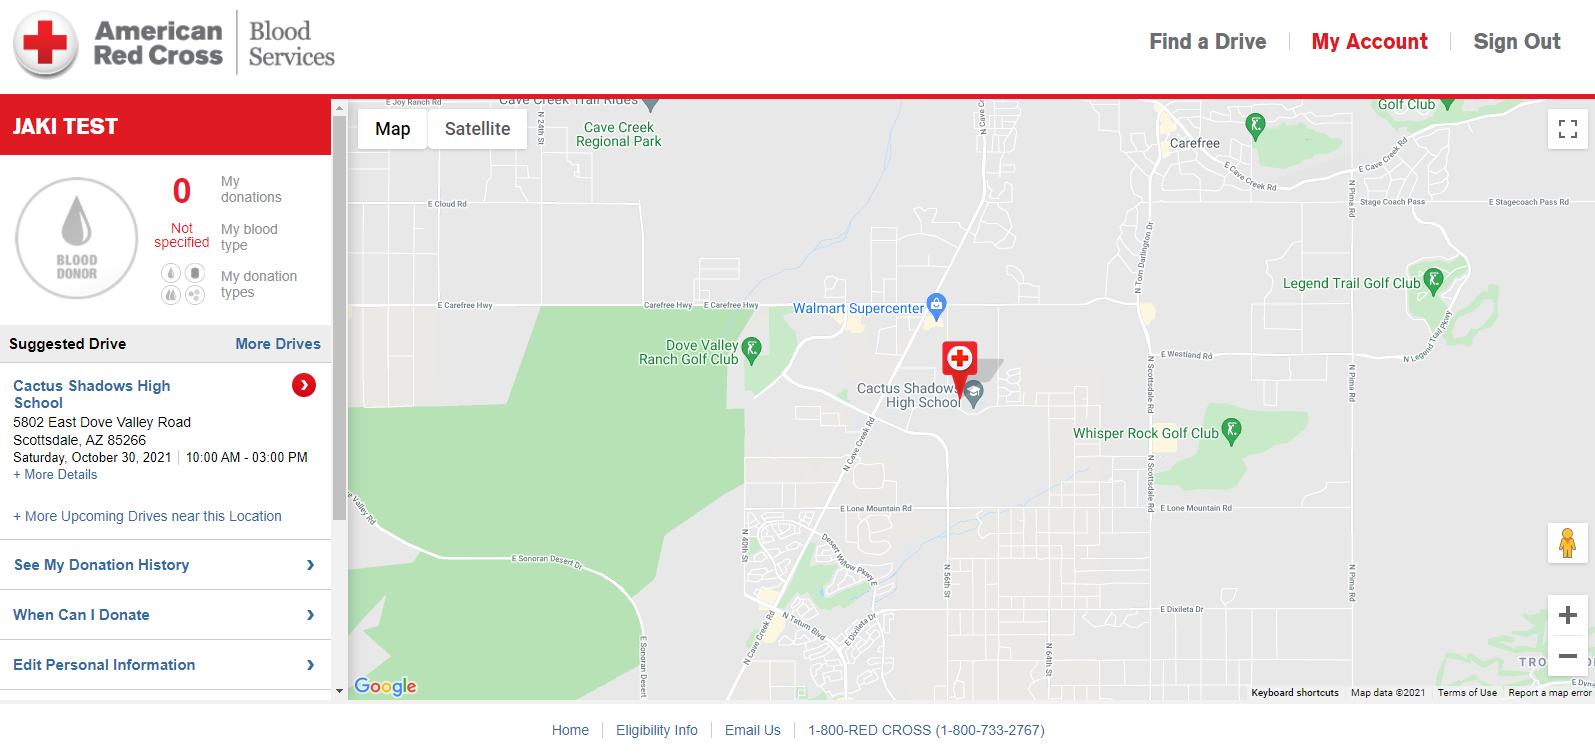
\includegraphics[scale=0.5]{slike/AmericanRedCrossPrimjer.PNG} %veličina slike u odnosu na originalnu datoteku i pozicija slike
			\centering
			\caption{Primjer web sučelja logiranog korisnika Američkog crvenog križa}
			\label{fig:AmericanRedCrossPrimjer}
		\end{figure}
		Ovo rješenje ima i nešto mjesta za kasniju nadogradnju. Jedna od mogućnosti je ugradnja podrške za notifikacije putem SMS poruka. Moguće je kasnije dodavanje i nešto poput nagradnog sistema za donore gdje bi donori svakim darivanjem krvi skupljali bodove koje bi mogli iskoristiti npr. za neke popuste kod nekih sponzora, besplatan ručak, ulaznicu u kino itd. 
		Naravno, kasnijih nadogradnji (i samih prilagodbi) može biti još, ovisno o željama i kasnijim potrebama korisnika rješenja, ukoliko su izvediva u sklopu ovog projekta.
		\eject

	
\chapter{Specifikacija programske potpore}

\section{Funkcionalni zahtjevi}

\noindent \textbf{Dionici:}

\begin{packed_enum}
	
	\item Korisnici	
	\item Javnost	
	\item Razvojni tim
	\item Naručitelj
	
\end{packed_enum}

\noindent \textbf{Aktori i njihovi funkcionalni zahtjevi:}


\begin{packed_enum}
	\item  \underbar{Neregistrirani/neprijavljeni korisnik(inicijator) može:}
	
	\begin{packed_enum}
		
		\item pregledati trenutno stanje zaliha
		\item se registrirati u sustav, stvoriti korisnički račun za koji su mu potrebni matični i kontakt podaci
		
	\end{packed_enum}
	
	\item  \underbar{Donor (inicijator) može:}
	
	\begin{packed_enum}
		
		\item pregledavati i mijenjati osobne podatke
		\item pregledavati povijest svojih doniranja
		\item iz aplikacije dobiti PDF potvrdu
		\item pregledati poruku u ovisnosti o trenutnom stanju zaliha krvi
		\item aktivirati račun aktivacijskim linkom i odabrati lozinku
		
	\end{packed_enum}
	
	\item  \underbar{Djelatnik banke (inicijator) može:}
	
	\begin{packed_enum}
		
		\item kreirati korisnički profil donora
		\item evidentirati svaki pokušaj doniranja (uspješan / neuspješan) 
		\item evidentirati privremeno ili trajno odbijanje
		\item evidentirati potrošnju krvi 
		\item aktivirati račun aktivacijskim linkom i odabrati lozinku
		\item vidjeti popis registriranih donora
		
	\end{packed_enum}
	\eject
	
	\item  \underbar{Administrator (inicijator) može:}
	
	\begin{packed_enum}
		
		\item definirati gornju i donju granicu optimalne količine krvi
		\item kreirati nove korisničke račune za ulogu djelatnika banke
		\item deaktivirati korisnički račun djelatnika banke ili donora
		\item vidjeti popis registriranih svih korisnika i njihovih osobnih podataka
		
	\end{packed_enum}
	
	\item  \underbar{Baza podataka (sudionik):}
	
	\begin{packed_enum}
		
		\item pohranjuje sve podatke o korisnicima i njihovim ovlastima
		\item pohranjuje trenutno stanje količine krvi,te donju i gornju granicu optimalne količine krvi
		\item pohranjuje sve podatke o donacijama krvi
	\end{packed_enum}
	
	\item  \underbar{Sustav za automatske poslove(inicijator) može:}
	
	\begin{packed_enum}
		
		\item slati email notifikacije donoru nakon 3 mjeseca od uspješnog darivanja ako je muškarac ili nakon 4 mjeseca ako je žensko
		
	\end{packed_enum}
\end{packed_enum}



\eject 



\subsection{Obrasci uporabe}

\subsubsection{Opis obrazaca uporabe}


\noindent \underbar{\textbf{UC1 - Pregledaj količine krvi}}
					\begin{packed_item}
	
						\item \textbf{Glavni sudionik: }Neregistrirani/neprijavljeni korisnik
						\item \textbf{Cilj:} Prikazati trenutnu količinu krvi u banci
						\item \textbf{Sudionici:} Baza podataka
						\item \textbf{Preduvjet:} -
						\item \textbf{Opis osnovnog tijeka:}
						
						\item[] \begin{packed_enum}
	
							\item Količine krvi su prikazane otvaranjem aplikacije, te njihove gornje i donje granice
							
						\end{packed_enum}

					\end{packed_item}

\noindent \underbar{\textbf{UC2 - Registriraj korisnika}}
					\begin{packed_item}
	
						\item \textbf{Glavni sudionik: }Neregistrirani/Neprijavljeni korisnik, djelatnik banke
						\item \textbf{Cilj:} Stvoriti korisnički račun donora za pristup sustavu
						\item \textbf{Sudionici:} Baza podataka
						\item \textbf{Preduvjet:} Djelatnik banke prijavljen 
						\item \textbf{Opis osnovnog tijeka:}
						
						\item[] \begin{packed_enum}
	
							\item Neregistriran/neprijavljen korisnik/djelatnik banke odabire opciju za registraciju novog donora
							\item Sustav otvara obrazac za registraciju
							\item Neregistriran/neprijavljen korisnik/djelatnik banke unosi potrebne podatke i odabire gumb za završetak registracije
							\item Sustav validira unesene podatke i sprema ih u bazu podataka
							\item Sustav generira email poruku s podacima o korisničkom računu i aktivacijskim linkom i šalje na mail adresu korisnika
							
						\end{packed_enum}
						
						\item  \textbf{Opis mogućih odstupanja:}
						
						\item[] \begin{packed_item}
	
							\item[2.a] Unos podataka u nedozvoljenom formatu ili unos neispravnog e-maila
							\item[] \begin{packed_enum}
								
								\item Korisnik dobiva obavijest o neuspjelom upisu i vraća ga na korak 2 osnovnog tijeka
								
							\end{packed_enum}
							
							
						\end{packed_item}
					\end{packed_item}
\eject 
\noindent \underbar{\textbf{UC3 - Prijavi se u sustav}}
					\begin{packed_item}
	
						\item \textbf{Glavni sudionik: }Donor
						\item \textbf{Cilj:} Prijava u sustav i dobivanje dodatnih mogućnosti aplikacije
						\item \textbf{Sudionici:} Baza podataka
						\item \textbf{Preduvjet:} Registracija
						\item \textbf{Opis osnovnog tijeka:}
						
						\item[] \begin{packed_enum}
	
							\item Donor unosi e-mail i lozinku u login formu te odabire akciju "Prijava"
							\item Sustav validira unesene podatke, provodi autentikaciju i autorizaciju korisnika
							\item Sustav otvara početni ekran aplikacije te korisniku 
							\item Pregledavanje ispisane obavijesti na ekranu 
							
						\end{packed_enum}
						\item  \textbf{Opis mogućih odstupanja:}
						
						\item[] \begin{packed_item}
	
							\item[2.a] Neispravan e-mail i/ili lozinka
							\item[] \begin{packed_enum}
								
								\item  Sustav obavještava korisnika o neuspjeloj prijavi i vraća ga u korak 1. osnovnog tijeka
								\end{packed_enum}
							\item[3.a] Prijeđena je donja optimalna granica ili je prošlo dovoljno vremena od prijašnje donacije
							\item[] \begin{packed_enum}
								
								\item  Sustav prikazuje obavijest da ima novih poruka u pretincu
							\end{packed_enum}
					\end{packed_item}
					\end{packed_item}
\noindent \underbar{\textbf{UC4 - Pregledaj osobne podatke}}
					\begin{packed_item}
	
						\item \textbf{Glavni sudionik: }Donor, Djelatnik
						\item \textbf{Cilj:} Prikazati osobne podatke donora
						\item \textbf{Sudionici:} Baza podataka
						\item \textbf{Preduvjet:} Donor/Djelatnik je prijavljen
						\item \textbf{Opis osnovnog tijeka:}
						
						\item[] \begin{packed_enum}
	
							\item Donor odabire opciju "Osobni podaci" ili Djelatnik odabere prikaz podataka donora
							\item Sustav dohvaća osobne podatke donora iz baze podataka te ih prikazuje
							
						\end{packed_enum}

					\end{packed_item}
\eject 
\noindent \underbar{\textbf{UC5 - Promjeni osobne podatke}}
					\begin{packed_item}
	
						\item \textbf{Glavni sudionik: }Donor, Djelatnik
						\item \textbf{Cilj:} Promjeniti matične i/ili kontakt podatke
						\item \textbf{Sudionici:} Baza podataka
						\item \textbf{Preduvjet:} Donor/Djelatnik je prijavljen
						\item \textbf{Opis osnovnog tijeka:}
						
						\item[] \begin{packed_enum}
	
							\item Donor/Djelatnik odabire opciju "Promijeni osobne podatke" kod prikaza osobnih podataka donora ili Djelatnik odabire opciju "Promjeni osobne podatke" kod prikaza svojih podataka
							\item Sustav otvara obrazac za promjenu osobnih podataka
							\item Donor/Djelatnik mijenja podatke i odabire opciju "Spremi promjene"
							
							\item Sustav ažurira bazu podataka
							
						\end{packed_enum}
					\end{packed_item}
\noindent \underbar{\textbf{UC6 - Pregledaj povijest darivanja}}
					\begin{packed_item}
	
						\item \textbf{Glavni sudionik: }Donor
						\item \textbf{Cilj:} Pregledati svoju povijest darivanja krvi
						\item \textbf{Sudionici:} Baza podataka
						\item \textbf{Preduvjet:} Donor je prijavljen
						\item \textbf{Opis osnovnog tijeka:}
						
						\item[] \begin{packed_enum}
	
							\item Donor odabire opciju "Povijest donacija"
							\item Sustav dohvaća povijest darivanja iz baze podataka te ju prikazuje
							
						\end{packed_enum}

					\end{packed_item}
\eject 
\noindent \underbar{\textbf{UC7 - Izvadi PDF potvrde}}
					\begin{packed_item}
	
						\item \textbf{Glavni sudionik:} Donor
						\item \textbf{Cilj:} Dobiti PDF potvrdu o doniranju
						\item \textbf{Sudionici:} Baza podataka
						\item \textbf{Preduvjet:} Donor je prijavljen i barem jedanput uspješno darovao krv
						\item \textbf{Opis osnovnog tijeka:}
						
						\item[] \begin{packed_enum}
	
							\item Donor odabire opciju "Povijest donacija"
							\item Sustav dohvaća povijest darivanja iz baze podataka te ju prikazuje
							\item Donor odabire opciju "Generiraj PDF" koja se nalazi uz svaki uspješan zapis doniranja krvi
							\item Sustav donoru šalje potvrdu na mail
							
						\end{packed_enum}

					\end{packed_item}

\noindent \underbar{\textbf{UC8 - Pregledaj poruke}}
					\begin{packed_item}
	
						\item \textbf{Glavni sudionik: }Donor
						\item \textbf{Cilj:} pregledati dospjelu poruku
						\item \textbf{Sudionici:} Baza podataka
						\item \textbf{Preduvjet:} Donor je prijavljen i nema trajnu/privremenu zabranu darivanja krvi
						\item \textbf{Opis osnovnog tijeka:}
						
						\item[] \begin{packed_enum}
	
							\item Donor odabire opciju "Pretinac"
							\item Sustav dohvaća poruke iz baze podataka i prikazuje ih
							\item Donor pregledava prikazane poruke
							
						\end{packed_enum}

					\end{packed_item}


\noindent \underbar{\textbf{UC9 - Smanji količinu krvi}}
					\begin{packed_item}
	
						\item \textbf{Glavni sudionik: }Djelatnik banke
						\item \textbf{Cilj:} slanje određenog broja jedinica krvi u vanjsku instituciju
						\item \textbf{Sudionici:} Baza podataka
						\item \textbf{Preduvjet:} Djelatnik je prijavljen
						\item \textbf{Opis osnovnog tijeka:}
						
						\item[] \begin{packed_enum}
							
							\item Djelatnik odabire opciju "Evidencija krvi"
							\item Sustav dohvaća podatke za svaku vrstu krvi
							\item Djelatnik odabire krvnu grupu čiju zalihu želi smanjiti
							\item Djelatnik upisuje količinu i naziv institucije u koju je potrebno poslati krv
							\item Djelatnik odabire akciju "Smanji zalihu"
							\item Sustav provjerava je li moguće provesti smanjivanje
							\item Sustav provodi smanjivanje u bazi podataka
						\end{packed_enum}
						\item  \textbf{Opis mogućih odstupanja:}
						
						\item[] \begin{packed_item}
							\item[4.a] Djelatnik je upisao ili preveliku količinu krvi ili manju od 1				
							\item[] \begin{packed_enum}
								
								\item  Sustav obavještava djelatnika o neispravnom unosu te ga vraća na korak 2 osnovnog tijeka
									\end{packed_enum}
							\item[5.a] Smanjivanjem se prešla donja granica optimalne količine krvi
							\item[] \begin{packed_enum}
								
								\item  Sustav šalje notifikaciju na mail adresu djelatniku banke i donoru(donoru se također šalje poruka u pretinac poruke)
							 

								
									\end{packed_enum}
								\end{packed_item}			
									
									
									
					\end{packed_item}
				


\noindent \underbar{\textbf{UC10 - Pregledaj popis donora}}
					\begin{packed_item}
	
						\item \textbf{Glavni sudionik: }Djelatnik banke, administrator
						\item \textbf{Cilj:} Prikazati popis svih registriranih donora
						\item \textbf{Sudionici:} Baza podataka
						\item \textbf{Preduvjet:} Djelatnik je prijavljen ili administrator je prijavljen
						\item \textbf{Opis osnovnog tijeka:}
						
						\item[] \begin{packed_enum}
	
							\item Djelatnik/administrator odabire opciju "Popis donora"
							\item Sustav djelatniku/administratoru dohvaća iz baze popis registriranih donora te ga prikazuje
						\end{packed_enum}

					\end{packed_item}



\noindent \underbar{\textbf{UC11 -{Aktiviraj račun}}}
\begin{packed_item}
	
	\item \textbf{Glavni sudionik: } {Neregistrirani/neprijavljeni korisnik, djelatnik banke}
	\item  \textbf{Cilj:} {Aktivirati račun}
	\item  \textbf{Sudionici:}{Baza podataka} 
	\item  \textbf{Preduvjet:}{Registracija}
	\item  \textbf{Opis osnovnog tijeka:}
	
	\item[] \begin{packed_enum}
		
		\item {Neregistrirani/neprijavljeni korisnik ili  djelatnik banke nakon klika na link u mailu vodi u aplikaciju}
		\item {Sustav ponovno renderira login stranicu gdje se traži da se unese nova proizvoljna lozinka} 
		\item {Neregistrirani/neprijavljeni korisnik ili  djelatnik banke se prijavljuje odabranom lozinkom}
	\end{packed_enum}
	
\end{packed_item}
\eject

\noindent \underbar{\textbf{UC12 -{Evidentiraj pokušaj doniranja}}}

\begin{packed_item}
	
	\item \textbf{Glavni sudionik: }{Djelatnik banke}
	\item  \textbf{Cilj:} {Evidentirati pokušaj doniranja}
	\item  \textbf{Sudionici:}{Baza podataka} 
	\item  \textbf{Preduvjet:}{Djelatnik banke je prijavljen i donor je registriran}
	\item  \textbf{Opis osnovnog tijeka:}
	
	\item[] \begin{packed_enum}
		
		\item {Djelatnik odabere opciju "Obavi donaciju" u prikazu popisa donira}
		\item {Sustav  prikazuje upitnik kojeg ispunjava djelatnik banke}
		\item {Djelatnik unosi mjesto doniranja}
		\item {Djelatnik banke sprema promjene}
		\item {Baza podataka se ažurira}
		\item {Sustav vraća uspješnost doniranja}
		\item {Sustav šalje email poruku s PDF potvrdom na mail donora}
		
	\end{packed_enum}
	\item  \textbf{Opis mogućih odstupanja:}
	
	\item[] \begin{packed_item}
		\item[5.a] {Donacija je uspješna}
		\item[] \begin{packed_enum}
			
			\item povećava se količina određene vrste krvi
			
		\end{packed_enum}
		\item[5.b] {Prešle su se gornje optimalne granice}
		\item[] \begin{packed_enum}
			
			\item šalju se notifikacije na mail djelatnika
			
		\end{packed_enum}
		
		\item[6.a] {\item[]\begin{packed_item}
		\item[•]Donor je bolovao ili boluje od teških kroničnih bolesti dišnog i probavnog sustava
		\item[•]Donor boluje od bolesti srca i krvnih žila, zloćudnih bolesti, bolesti jetre, AIDS-a, šećerne bolesti 
		\item[•]Donor je ovisnik o alkoholu ili drogama 
		\item[•]Donor ima spolne odnose s drugim muškarcima 
		\item[•]Donor često mijenja seksualne partnere
		\item[•]Donor je uzimao drogu intravenskim putem
		\item[•]Donor je liječen zbog spolno prenosivih bolesti 
		\item[•]Donor je HIV pozitivan
		\item[•]Donor je seksualni partner gore navedenih osoba
		\end{packed_item}}
		\item[] \begin{packed_enum}
			
			\item Donor se trajno odbija
			\item U bazu se zapisuje trajno odbijanje za određenog donora
		\end{packed_enum}
\eject
		\item[6.b] {\item[]\begin{packed_item}
		\item[•]Tjelesna težina je ispod 55kg
		\item[•]Tjelesna temperatura je iznad 37°C 
		\item[•]Krvni tlak sistolički je ispod 100, a dijastolički ispod 60 
		\item[•]Puls je ispod 50 ili iznad 100 otkucaja u minuti 
		\item[•]Hemoglobin muškaraca ispod 135g/L, a žena ispod 125g/L
		\item[•]Donor trenutno uzima antibiotike ili druge lijekove      
		\item[•]Donor je konzumirao alkohol unutar 8 sati 
		\item[•]Donor ima akutno bolesno stanje
		\item[•]Donor je žena za vrijeme menstruacije ili trudnoće 
	    \item[•]Donor je obavljao opasne poslove tog dana
	    \item[•]Donor je muškarac i nije prošlo 3 mjeseca od zadnjeg doniranja
	    \item[•]Donor je žena i nije prošlo 4 mjeseca od zadnjeg doniranja\end{packed_item}}
		\item[] \begin{packed_enum}
			
			\item Donor se privremeno odbija
			\item U bazu se zapisuje privremeno odbijanje za određenog donora
			\end{packed_enum}
		
		
	\end{packed_item}
	
\end{packed_item}
\eject 

\noindent \underbar{\textbf{UC13 -{Obriši donora}	}}
\begin{packed_item}
	
	\item \textbf{Glavni sudionik: }{Administrator}
	\item  \textbf{Cilj:} {deaktivirati kor. račun donora}
	\item  \textbf{Sudionici:}{Baza podataka}
	\item  \textbf{Preduvjet:}{Administrator prijavljen}
	\item  \textbf{Opis osnovnog tijeka:}
	
	\item[] \begin{packed_enum}
		
		\item {Administrator odabire opciju "Popis donora"}
		\item {Sustav prikazuje popis registriranih donora} 
		\item {Administrator odabire opciju "Obriši donora"}
		\item {Sustav briše donora, ali ostaje zapis o njegovim donacijama}
		\item {Baza se ažurira}
	\end{packed_enum}
	
\end{packed_item}


\noindent \underbar{\textbf{UC14 -{Definiraj optimalne granice}	}}

\begin{packed_item}
	
	\item \textbf{Glavni sudionik: }{Administrator}
	\item  \textbf{Cilj:} {Definirati gornju i donju granicu optimalnih količina krvi za pojedinu grupu}
	\item  \textbf{Sudionici:}{Baza podataka}
	\item  \textbf{Preduvjet:}{Administrator je prijavljen}
	\item  \textbf{Opis osnovnog tijeka:}
	
	\item[] \begin{packed_enum}
		
		\item {Administrator odabire opciju "Definiraj granice"}
		\item {Sustav prikazuje trenutno određene granice za pojedinu vrstu krvi} 
		\item {Administrator definira granice za pojedinu vrstu krvi}
		\item {Administrator sprema promjene}
		\item {Baza se ažurira}
		\end{packed_enum}
	\item  \textbf{Opis mogućih odstupanja:}
	
		\item[] \begin{packed_item}
		
			\item[4.b] {Prešle su se gornje optimalne granice}	
				\item[] \begin{packed_enum}
			
				\item Sustav šalje notifikacije na mail djelatnika			
				\end{packed_enum}
			\item[4.c] {Prešle su se donje optimalne granice}	
				\item[] \begin{packed_enum}
			
				\item Sustav šalje notifikacije na mail djelatnika i donora ako se radi o njegovoj krvnoj grupi (također donoru se šalje poruka u pretinac za poruke)
				\end{packed_enum}
		
		
			\end{packed_item}
\end{packed_item}

\eject
\noindent \underbar{\textbf{UC15 -{Pregledaj popis djelatnika}	}}

\begin{packed_item}
	
	\item \textbf{Glavni sudionik: }{Administrator}
	\item  \textbf{Cilj:} {Prikazati popis svih djelatnika banke}
	\item  \textbf{Sudionici:}{Baza podataka} 
	\item  \textbf{Preduvjet:}{Administrator je prijavljen}
	\item  \textbf{Opis osnovnog tijeka:}
	
	\item[] \begin{packed_enum}
		
		\item {Administrator odabire opciju "Popis djelatnika"}
		\item {Sustav prikazuje popis svih djelatnika banke}
		\end{packed_enum}
\end{packed_item}


\noindent \underbar{\textbf{UC16 -{Obriši djelatnika banke}}}

\begin{packed_item}
	\item \textbf{Glavni sudionik: }{Administrator}
	\item  \textbf{Cilj:} {Deaktivirati kor. račun djelatnika banke}
	\item  \textbf{Sudionici:}{Baza podataka}
	\item  \textbf{Preduvjet:}{Administrator prijavljen}
	\item  \textbf{Opis osnovnog tijeka:}
	
	\item[] \begin{packed_enum}
		
		\item {Administrator odabire opciju "Popis djelatnika"}
		\item {Sustav vraća popis djelatnika banke}
		\item {Administrator odabire opciju "Obriši djelatnika banke"}
		\item {Sustav briše djelatnika, ali ostaju zapisi o njegovim provedenim donacija i evidentiranju smanjenja količina krvi}
		\item {Baza se ažurira}
	\end{packed_enum}
	
\end{packed_item}


\noindent \underbar{\textbf{UC17 -{Kreiraj kor. računa djelatnika banke}	}}

\begin{packed_item}
	
	\item \textbf{Glavni sudionik: }{Administrator}
	\item  \textbf{Cilj:} {Kreirati računa djelatnika banke}
	\item  \textbf{Sudionici:}{Baza podataka}
	\item  \textbf{Preduvjet:}{Administrator je prijavljen}
	\item  \textbf{Opis osnovnog tijeka:}
	
	\item[] \begin{packed_enum}
		
		\item {Administrator odabire opciju "Dodaj djelatnika"}
		\item {Sustav prikazuje formu za kreiranje računa koju popunjava administrator} 
		\item {Odabire gumb "Registriraj"}
		\item {Baza podataka se ažurira}
		\item {Sustav šalje aktivacijski link na email djelatnika banke}
	\end{packed_enum}
	
	\item  \textbf{Opis mogućih odstupanja:}
	
	\item[] \begin{packed_item}
		
		\item[2.a]{Sva polja nisu ispunjena}
		\item[] \begin{packed_enum}
			
			\item Sustav obavještava administratora da unese sve podatke
			
		\end{packed_enum}
	\end{packed_item}
\end{packed_item}
\eject 

\noindent \underbar{\textbf{UC18 -{Pošalji notifikacije nakon 3/4 mjeseca}	}}
\begin{packed_item}
	
	\item \textbf{Glavni sudionik: }{Sustav za automatske poslove}
	\item  \textbf{Cilj:} {Poslati notifikaciju donoru}
	\item  \textbf{Sudionici:}{Baza podataka, donor}
	\item  \textbf{Preduvjet:}{Prošlo 3 ili 4 mjeseca od uspješnog darivanja}
	\item  \textbf{Opis osnovnog tijeka:}
	
	\item[] \begin{packed_enum}
		
		\item {Sustav svakodnevno provjerava uspješna doniranja od prije 3 mjeseca za muškarce i od prije 4 mjeseca za žene}
		\item {Sustav svim donorima koji zadovoljavaju uvjet šalje email notifikacije da mogu doći ponovno donirati krv}
		\item {Sustav svim donorima koji zadovoljavaju uvjet šalje poruke u njihov pretinac poruka da mogu doći ponovno donirati krv}
		
	\end{packed_enum}
	
\end{packed_item}


\subsubsection{Dijagrami obrazaca uporabe}
\begin{figure}[H]
			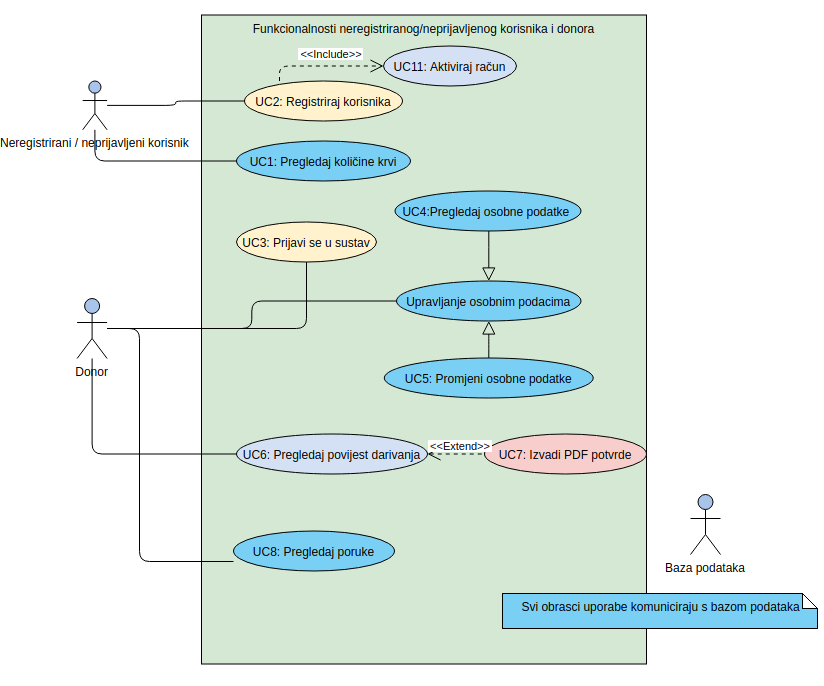
\includegraphics[scale=0.6]{dijagrami/Funkcionalnosti_korisnika_donora.png} %veličina slike u odnosu na originalnu datoteku i pozicija slike
			\centering
			\caption{Dijagram obrasca uporabe, funkcionalnost neregistriranog / neprijavljenog korisnika i donora}
			\label{fig:Funkcionalnosti_korisnika_donora}
\end{figure}

\begin{figure}[H]
			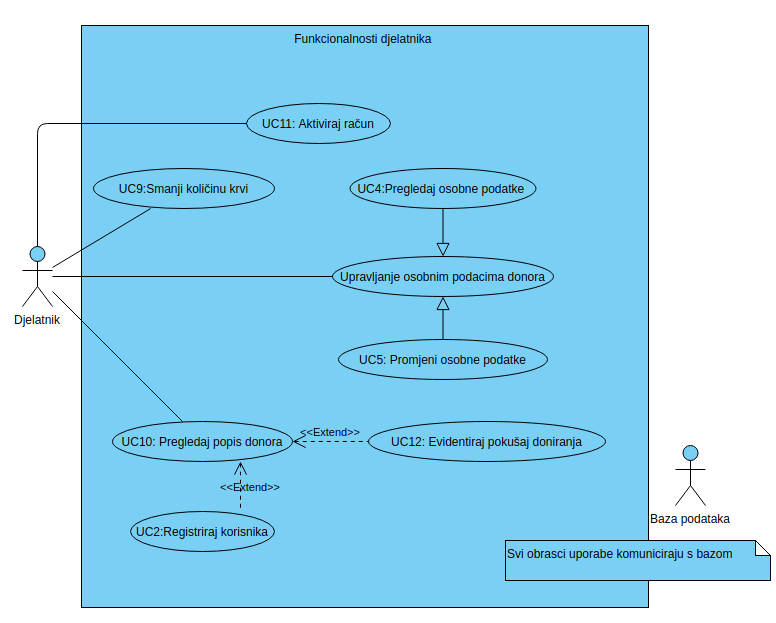
\includegraphics[scale=0.6]{dijagrami/Funkcionalnosti_djelatnika_donora.png} %veličina slike u odnosu na originalnu datoteku i pozicija slike
			\centering
			\caption{Dijagram obrasca uporabe, funkcionalnost djelatnika}
			\label{fig:Funkcionalnosti_djelatnika_donora}
\end{figure}

\begin{figure}[H]
			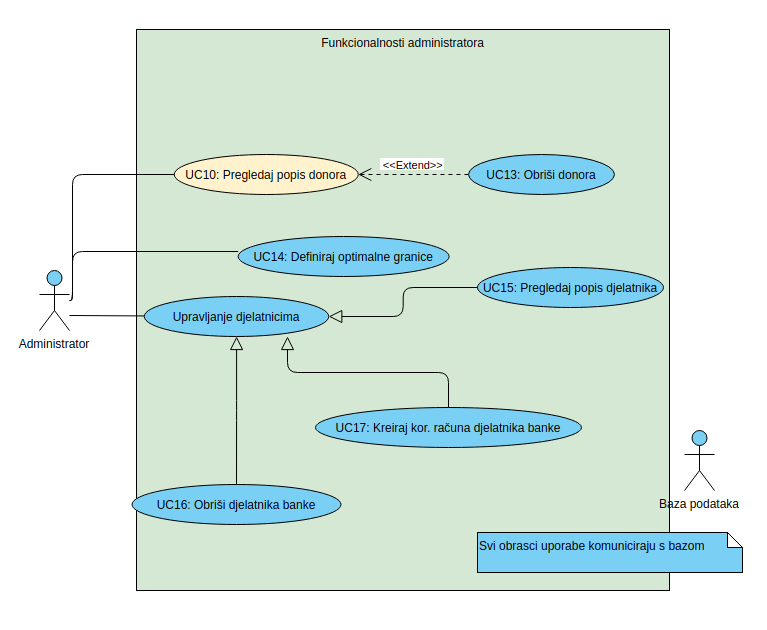
\includegraphics[scale=0.6]{dijagrami/Funkcionalnosti_admina.png} %veličina slike u odnosu na originalnu datoteku i pozicija slike
			\centering
			\caption{Dijagram obrasca uporabe, funkcionalnost administratora}
			\label{fig:Funkcionalnosti_admina}
\end{figure}

\begin{figure}[H]
			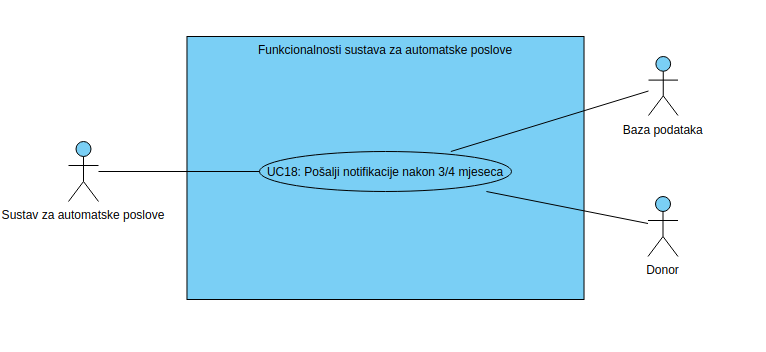
\includegraphics[scale=0.6]{dijagrami/Funkcionalnosti_auto.png} %veličina slike u odnosu na originalnu datoteku i pozicija slike
			\centering
			\caption{Dijagram obrasca uporabe, funkcionalnost sustava za automatske poslove}
			\label{fig:Funkcionalnosti_auto}
\end{figure}

\eject
		
\subsection{Sekvencijski dijagrami}

\textbf{Obrazac uporabe UC8 - Dobivanje poruke stanja zalihe krvi}

Donor, koji nema trajnu zabranu darivanja krvi, kod svakog spajanja u sustav dobiva poruku u ovisnosti o trenutnom stanju zaliha krvi. Poslužitelj dohvaća podatke iz baze podataka i prema zadanim granicama vraća jednu od tri poruka. Poruke mogu biti: stanje zaliha ispod optimalne granice; stanje zaliha je optimalno; stanje zaliha je iznad gornje optimalne granice.

\begin{figure}[H]
	\centering
	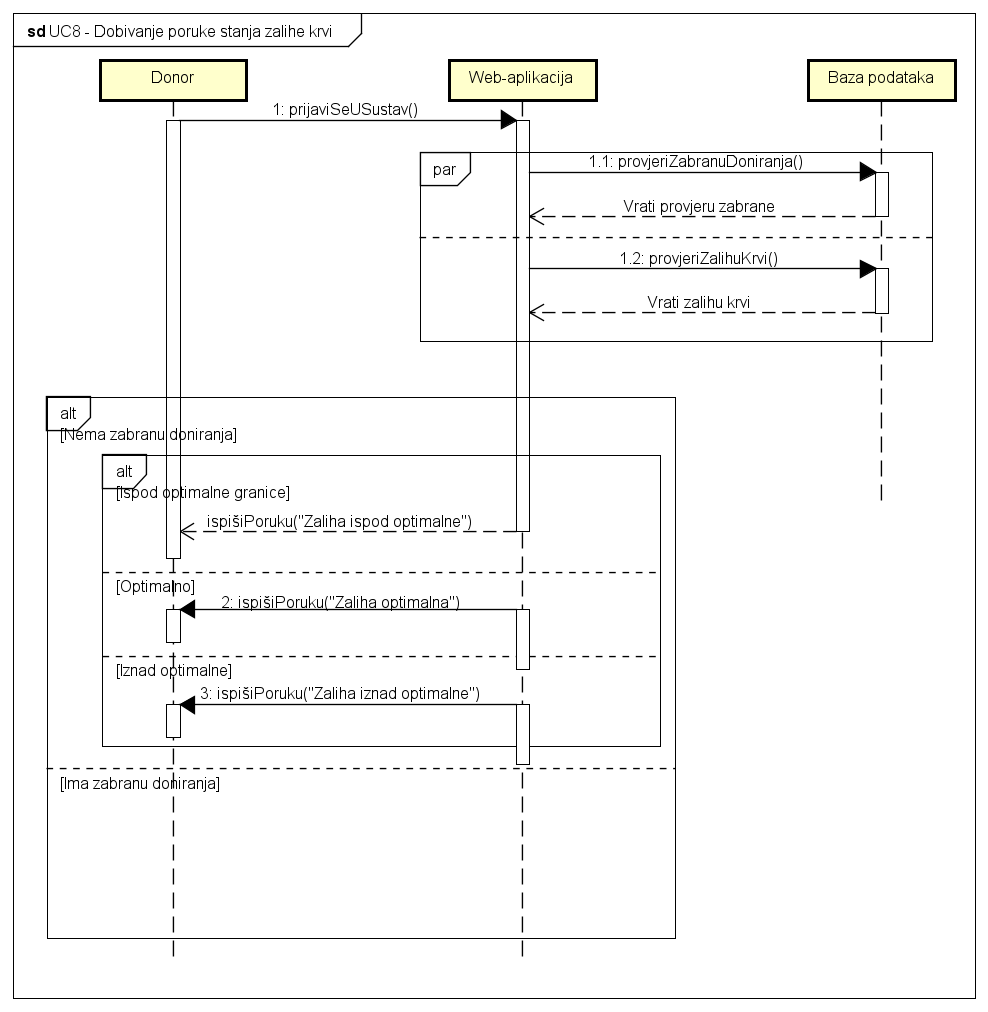
\includegraphics[width=\textwidth, scale=0.4]{dijagrami/UC8_Dobivanje poruke stanja zalihe krvi.png}
	\caption{Sekvencijski dijagram za UC8}
	\label{fig:UC8_Dobivanje poruke stanja zalihe krvi}
\end{figure}
\eject

\textbf{Obrazac uporabe UC9 - Evidentiranje "potrošnje" krvi}

Djelatnik banke može evidentirati "potrošnju" krvi odnosno slanje određenog broja jedinica krvi u vanjsku instituciju. U bazi podataka se smanjuje količina određene vrste krvi i ako se prešla donja granica šalje se mail djelatniku.

\begin{figure}[H]
	\centering
	\includegraphics[width=\textwidth, scale=0.4]{dijagrami/UC9_Evidentiranje_potrošnje_ krvi.png}
	\caption{Sekvencijski dijagram za UC9}
\end{figure}

\eject 
\textbf{Obrazac uporabe UC12 - Evidentiranje pokušaja doniranja}

Djelatnik banke evidentira i uspješne i neuspješne pokušaje doniranja. Na temelju zdravstvenog stanja donor može pristupiti doniranju, ali može i biti privremeno ili trajno odbijen. Baza podataka se ažurira, zapisuje se pokušaj doniranja krvi i ako je uspješan poveća se razina određene vrste krvi.

\begin{figure}[H]
	\centering
	\includegraphics[width=\textwidth]{dijagrami/UC12_Evidentiranje pokušaja doniranja.png}
	\caption{Sekvencijski dijagram za UC12}
\end{figure}
\eject

\textbf{Obrazac uporabe UC14 - Definiranje optimalnih granica}

Za svaku krvnu grupu administrator sustava definira gornju i donju granicu optimalne količine. Administratoru se prikazuju trenutne granice za pojedinu vrstu krvi. Zatim on ih on može mijenjati i promjene se spremaju i bazu podataka. Ako je prijeđena gornja granica šalje se mail djelatniku. Ako je prijeđena donja granica šalje se mail djelatniku i poruke donorima.

\begin{figure}[H]
	\centering
	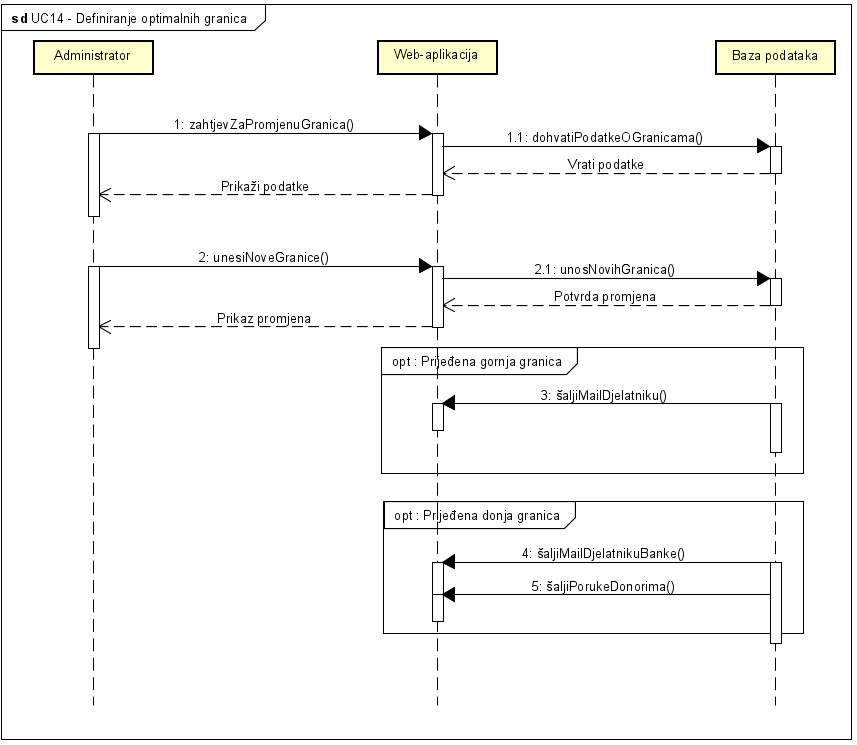
\includegraphics[width=\textwidth]{dijagrami/UC14_Definiranje optimalnih granica.png}
	\caption{Sekvencijski dijagram za UC14}
\end{figure}
\eject

\section{Ostali zahtjevi}

\begin{packed_item}
	
	\item Sustav treba biti implementiran kao web aplikacija koja je prilagođena različitim veličinama ekrana. (responsive web design)
	\item Sustavu trebaju moći pristupati tri vrste korisnika (administrator, djelatnik banke i donor). Svaki korisnik se treba ovjeravati korisničkim imenom i lozinkom.
	\item Donori trebaju imati mogućnost sami kreirati svoj korisnički račun kao i djelatnici banke u slučaju da donor sam nije napravio korisnički račun prije prvog darivanja.
	\item Administratori trebaju imati mogućnost kreiranja korisničkog računa za djelatnike banke.
	\item Novi korisnici trebaju dobiti aktivacijski link na svoj mail, donori uz aktivacijski link trebaju dobiti i donorId koji će koristiti kao korisničko ime.
	\item Prilikom aktivacije korisničkog računa, korisnici trebaju imati mogućnost odabrati svoju lozinku.
	\item Sustav treba omogućiti rad više korisnika u stvarnom vremenu.
	\item Neispravno korištenje sustava ne smije narušiti rad sustava.
	\item Korisničko sučelje treba biti intuitivno, tako da se korisnici mogu koristiti sustavom bez dodatnih uputa.
	\item Sustav treba podržavati hrvatsku abecedu pri unosu i prikazu tekstualnog sadržaja.
	\item Veza s bazom podataka mora biti zaštićena.

\end{packed_item}






	\chapter{Arhitektura i dizajn sustava}
		
		Arhitekturu našeg sustava možemo podijeliti na tri podsustava:	
		\begin{itemize}
		\item 	\textit{Web preglednik}
		\item 	\textit{Baza podataka}
		\item 	\textit{Web poslužitelj}		
		\end{itemize}
		
		\begin{figure}[H]
			\centering
			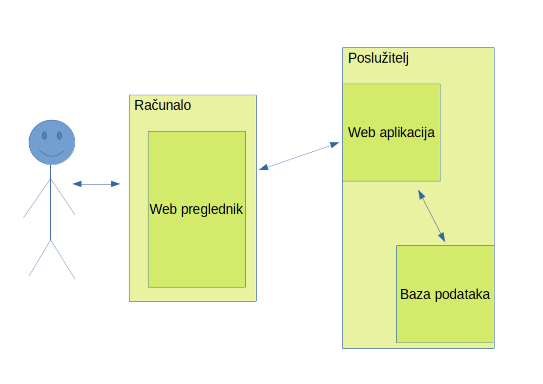
\includegraphics[width=\textwidth, scale=2.0]{slike/arhitektura.png}
			\caption{Arhitektura sustava}
			\label{fig:arhitektura}
		\end{figure}
\eject
	
	
	
	\underbar{ \textit{Web preglednik} }{je program koji korisniku omogućuje pregled web-stranica i multi-medijalnih sadržaja vezanih uz njih. Korisnik putem web preglednika šalje zahtjeve na obradu poslužitelju.}

	\underbar{ \textit{Baza podataka}}{ je zbirka zapisa pohranjenih u računalu na sustavan način, tako da joj se računalni program može obratiti prilikom odgovaranja na problem. Web poslužitelj komunicira s bazom podataka te povlači potrebne zapise iz nje.}
	
	\underbar{ \textit{Web poslužitelj}}{ je srce našeg sustava. Njegova zadaća je komunikacija klijenta s aplikacijom te bazom podataka. Pri komunikaciji koristi HTTP protokol.Korisnik i aplikacija razmjenjuju HTTP zahtjeve (eng. HTTP request) i HTTP odgovore (HTTP response). Radi jednostavnosti, baza podataka je također smještena na poslužitelju.}\\
	Korisnik kroz grafičko sučelje, odnosno frontend, šalje zahtjeve na REST pristupne točke backenda. Tada backend procesuira zahtjev i ako je potrebno komunicira s bazom podataka. Nakon konstrukcije, backend šalje odgovor frontendu u obliku JSON objekta, a frontend procesuira odgovor i promjene prikazuje korisniku u obliku HTML stranice.
\eject
	Programski jezik kojeg smo odabrali za izradu naše web aplikacije je Java zajedno s Spring radnim okvirom te programski jezik JavaScript u sklopu React-a. Odabrana razvojna okruženja su Eclipse i IntelliJ IDEA. Za aplikaciju je odabrana višeslojna arhitektura temeljena na \textbf{MVC} (Model - View - Controller) arhitekturnom stilu te uslužnoj arhitekturi. Podjela slojeva možemo napraviti na idući način:
	\begin{figure}[H]
			\centering
			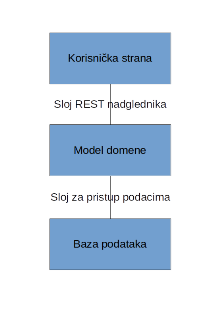
\includegraphics[scale=0.9]{slike/arhitektura2.png}
			\caption{Podjela slojeva}
			\label{fig:slojevi}
		\end{figure}
	\begin{itemize}
		\item 	\textit{sloj korisničke strane} - korisničko sučelje
		\item 	\textit{sloj nadglednika} - REST nadglednici
		\item 	\textit{sloj domene}	- model podataka iz domene primjene
		\item 	\textit{sloj za pristup podacima} - posrednik između sloja domene i baze podataka
		\item 	\textit{sloj baze podataka} - pohrana podataka	
		\end{itemize}

\eject	{Ovakva arhitektura odabrana je zbog poželjnih svojstava MVC arhitekturnog stila i višeslojne arhitekture: razvoj pojedinih slojeva je jednostavniji i u velikom stupnju nezavisan od razvoja drugih slojeva. Također komunikacija frontenda i backenda ostvarena je primjenom REST arhitekturnog stila. Zbog toga su i frontend i backend neovisni o jeziku implementacije, što potiče ponovnu uporabu. }
	
	 {Model-View-Controller se sastoji od:}
	\begin{itemize}
		\item 	\textbf{Model} {je centralni dio aplikacije, koja obuhvaća promjenljivu (dinamičku) strukturu podataka, direktno upravljanje podacima, logikom i pravilima aplikacije}
		\item 	\textbf{View}{ je bilo koji izlazni prikaz podataka u korisničkom okruženju, pri čemu se isti podaci mogu prikazati na više načina}
		\item 	\textbf{Controller} {ulazne podatke pretvara u komande koje upravljaju modelom ili prikazom podataka u korisničkom okruženju}
	\end{itemize}
	
		\begin{figure}[H]
			\centering
			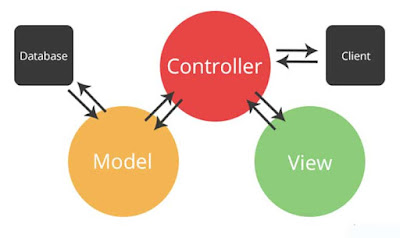
\includegraphics[width=100mm, scale=0.1]{slike/MVC.jpeg}
			\caption{MVC model}
			\label{fig:arhitektura}
		\end{figure}
\eject

		

				
		\section{Baza podataka}
			
			
			
		Za potrebe našeg sustava koristit ćemo relacijsku bazu podataka koja svojom strukturom olakšava modeliranje stvarnog svijeta. Gradivna jedinka baze je relacija, odnosno tablica koja je definirana svojim imenom i skupom atributa. Zadaća baze podataka je brza i jednostavna pohrana, izmjena i dohvat podataka za daljnju obradu.
Baza podataka ove aplikacije sastoji se od sljedećih entiteta: 
\begin{itemize}
		\item korisnikAplikacije
		\item uloge
		\item pokusajDoniranja
		\item krvnaVrsta
		\item potrosnjaKrvi
		\item zdravstveniPodaci
		\item doniranjeZdravljeOdgovori
		
	\end{itemize}

		\eject
			\subsection{Opis tablica}
			

				\textbf{korisnikAplikacije \textit{•}}
				 Ovaj entitet predstavlja sve korisnike aplikacije (admin, djelatnik, donor) i diferencira ih pomoću ulogaId što je referenca na tablicu uloga.Za admina i djelatnika postoje atributi : ime, prezime, oib, email dok su ostale vrijednosti null. Kod stvaranja atributa trajnoOdbijanjeDarivanja je false, a razlogOdbijanja je null ,ako se korisniku odbije darivanje zauvijek onda se ti atributi mijenjaju. One-to-many veza s pokusajDoniranja preko korisnikID dvaput, One-to-many veza s potrosnjaKrvi preko korisnikId, many-to-one veza s uloge preko ulogaId i many-to-one veza s krvnaVrsta preko krvId.

				
				\begin{longtblr}[
					label=none,
					entry=none
					]{
						width = \textwidth,
						colspec={|X[15,l]|X[6, l]|X[20, l]|}, 
						rowhead = 1,
					} %definicija širine tablice, širine stupaca, poravnanje i broja redaka naslova tablice
					\hline \multicolumn{3}{|c|}{\textbf{korisnikAplikacije}}	 \\ \hline[3pt]				
					\SetCell{LightGreen}korisnikId & VARCHAR & id pomoću kojeg se korisnik prijavljuje u sustav (jednako donorId za donore)\\ \hline
					lozinka	& VARCHAR &  hash korisničke lozinke 	\\ \hline 
					ime & VARCHAR	&  ime korisnika		\\ \hline 
					prezime & VARCHAR	& prezime korisnika	\\ \hline 
					mjestoRodenja & VARCHAR & mjesto rođenja (nullable) \\ \hline
					oib & VARCHAR & oib korisnika \\ \hline
					adresaStanovanja & VARCHAR & adresa stanovanja (nullable) \\ \hline
					mjestoZaposlenja & VARCHAR & firma u kojoj je korisnik zaposlen (nullable) \\ \hline
					email & VARCHAR & email na koji korisniku dolaze korisne informacije (nullable) \\ \hline 
					brojMobitelaPrivatni & VARCHAR	&  privatni broj korisnika	(nullable)	\\ \hline
					brojMobitelaPoslovni & VARCHAR	&  broj na koji korisniku dolaze korisne infromacije poslovni(nullable)\\ \hline
                     datumRodenja & DATE &  datum rođenja	\\ \hline
                     \SetCell{LightBlue}krvId & INT & vrsta krvi donora \\ \hline
                     trajnoOdbijenoDarivanje & BOOLEAN &  true ako je korisniku zabranjeno trajno darivanje, false ako nije \\ \hline
					 \SetCell{LightBlue}ulogaId & BIGINT &  oznaka uloge korisnika \\ \hline 
					aktivacijskiKljuc & VARCHAR(10) & aktivacijski ključ koji služi za aktivaciju računa \\
\hline		
					\end{longtblr}
				
				\textbf{uloge \textit{•}}
				entitet koji sadrži dva atributa, id za oznaku rednog broja uloge i ulogaName za ime 						uloge
				One-to-many veza s korisnikAplikacije preko ulogaId.
				\begin{longtblr}[
					label=none,
					entry=none
					]{
						width = \textwidth,
						colspec={|X[6,l]|X[6, l]|X[20, l]|}, 
						rowhead = 1,
					} %definicija širine tablice, širine stupaca, poravnanje i broja redaka naslova tablice
					\hline \multicolumn{3}{|c|}{\textbf{Uloge}}	 \\ \hline[3pt]
					\SetCell{LightGreen}ulogaId & BIGINT & označava id uloge \\ \hline
					ulogaName	& VARCHAR & naziv uloge	\\ \hline 
					
				\end{longtblr}
	\eject
				\textbf{pokusajDonacije\textit{•}}
				-entitet koji predstavlja pokušaj doniranja, sadrži podatke o datumu, mjestu, darivatelju, djelatniku, uspješnosti i razlogu odbijanja ako je uspješnost false.
				Many-to-one veza preko korisnikIdDjelatnika s korisnikAplikacije , Many-to-one veza preko korisnikIdDonora s korisnikAplikacije, one-to-many veza s doniranjeZdravljeOdgovori reko brDoniranja.
				
				\begin{longtblr}[
					label=none,
					entry=none
					]{
						width = \textwidth,
						colspec={|X[15,l]|X[6, l]|X[20, l]|}, 
						rowhead = 1,
					} %definicija širine tablice, širine stupaca, poravnanje i broja redaka naslova tablice
					\hline \multicolumn{3}{|c|}{\textbf{pokusajDonacije}}	 \\ \hline[3pt]
					\SetCell{LightGreen}brDoniranja & BIGINT & redni broj donacije\\ \hline
					datum & DATE & datum donacije \\ \hline
					mjestoDarivanja	& VARCHAR & opisno mjesto donacije	\\ \hline 
					\SetCell{LightBlue}korisnikIdDjelatnika & VARCHAR & identifikator djelatnika \\ \hline
					\SetCell{LightBlue}korisnikId & VARCHAR & identifikator donora \\ \hline

					uspjeh	& BOOLEAN & oznaka uspješnosti darivanja  	\\ \hline 			
					
				\end{longtblr}
				
				\textbf{krvnaVrsta\textit{•}}
				
				- entitet čuva podatke o zalihi i predviđenim gornjim i donjim granicama za sve krvne grupe.  one-to-many veza s potrosnjaKrvi preko krvId i one-to-many veza s korisnikAplikacije preko krvId.
				\begin{longtblr}[
					label=none,
					entry=none
					]{
						width = \textwidth,
						colspec={|X[15,l]|X[6, l]|X[20, l]|}, 
						rowhead = 1,
					} %definicija širine tablice, širine stupaca, poravnanje i broja redaka naslova tablice
					\hline \multicolumn{3}{|c|}{\textbf{krvnaVrsta}}	 \\ \hline[3pt]
					\SetCell{LightGreen}krvId & SERIAL & identifikator krvne grupe \\ \hline
					imeKrvneGrupe & VARCHAR & naziv krvne grupe \\ \hline
					gornjaGranica & INT & gornja granica dopuštene količine krvi u jedinicama\\ \hline

					donjaGranica	& INT & donja granica dopuštene količine krvi u jedinicama  	\\ \hline 
					trenutnaZaliha	& INT &  trenutna zaliha konkretne krvne grupe u jedinicama 	\\ \hline 
					
					
				\end{longtblr}
\eject			
				
				\textbf{potrosnjaKrvi\textit{•}}
				
				entitet koji prati isporuke krvi . 
				Many-to-one veza s korisnikAplikacije preko korisnikIdDjelatnika i Many-to-one veza s krvnaVrsta preko krvId.

				\begin{longtblr}[
					label=none,
					entry=none
					]{
						width = \textwidth,
						colspec={|X[15,l]|X[6, l]|X[20, l]|}, 
						rowhead = 1,
					} %definicija širine tablice, širine stupaca, poravnanje i broja redaka naslova tablice
					\hline \multicolumn{3}{|c|}{\textbf{potrosnjaKrvi}}	 \\ \hline[3pt]
					\SetCell{LightGreen} idPotrosnje & SERIAL & redni broj isporuke krvi \\ \hline
					timestampPotrosnje & TIMESTAMP & timestamp potrošnje \\ \hline
					\SetCell{LightBlue}krvId & INT & id krvne grupe \\ \hline
					količinaJedinica & INT &  broj jedinica koje su se potrošili \\ \hline 
					
					\SetCell{LightBlue}korisnikIdDjelatnika & VARCHAR &  identifikator djelatnika koji je inicirao slanje krvi bolnici	\\ \hline 
					lokacijaPotrosnje & VARCHAR & opisna lokacija kamo ide isporuka krvi \\ \hline
					
				\end{longtblr}
				
				\textbf{zdravstveniPodaci\textit{•}}
				
				entitet koji sprema sve moguće zdravstvene podatke koji se pitaju korisnika u upitniku. Oni sadrže svoj id, koji se sam generira u tablici, opis zdravstvenog podatka i težinu kriterija odnosno, 0 ako se na temelju toga podatka trajno odbija darivanje i 1 ako se privremeno odbija, inače null.
				One-to-many veza s doniranjeZdravljeOdgovori preko idZdravstvenih.
				\begin{longtblr}[
					label=none,
					entry=none
					]{
						width = \textwidth,
						colspec={|X[10,l]|X[6, l]|X[20, l]|}, 
						rowhead = 1,
					} %definicija širine tablice, širine stupaca, poravnanje i broja redaka naslova tablice
					\hline \multicolumn{3}{|c|}{\textbf{zdravstveniPodaci}}	 \\ \hline[3pt]
					\SetCell{LightGreen}idZdravstvenih & SERIAL & id zdravstvenog podatka \\ \hline
					zdravstveniPodatak & VARCHAR & opis zdravstvenog podatka koji se ispituje
					npr. osoba teži manje od 55 kg \\ \hline
					tezinaKriterija 	& INT &  tezina kriterija ( 0 za trajno, 1 za privremeno) 	\\ \hline 

					
				\end{longtblr}
\eject				
				\textbf{doniranjeZdravljeOdgovori\textit{•}}
				
				entitet koji služi kao spremište odgovora korisnika koji su došli donirati krv.
				Many-to-one veza s zdravstveniPodaci preko idZdravstvenih. Many-to-one veza s pokusajDoniranja preko brDoniranja.
				\begin{longtblr}[
					label=none,
					entry=none
					]{
						width = \textwidth,
						colspec={|X[10,l]|X[6, l]|X[20, l]|}, 
						rowhead = 1,
					} %definicija širine tablice, širine stupaca, poravnanje i broja redaka naslova tablice
					\hline \multicolumn{3}{|c|}{\textbf{doniranjeZdravljeOdgovori}}	 \\ \hline[3pt]
					\SetCell{LightGreen} brDoniranja & INT & brDoniranja iz tablice pokusajDoniranja \\ \hline
					\SetCell{LightGreen} idZdravstvenih & INT &  idZdravstvenih iz tablice zdravstveni podaci \\ \hline
					odgovorDonora & BOOLEAN & odgovor donora na zdravstveni podatak pod idZdravstvenih\\ \hline
					
				\end{longtblr}
			
			\subsection{Dijagram baze podataka}
				\begin{figure}[H]
	\centering
	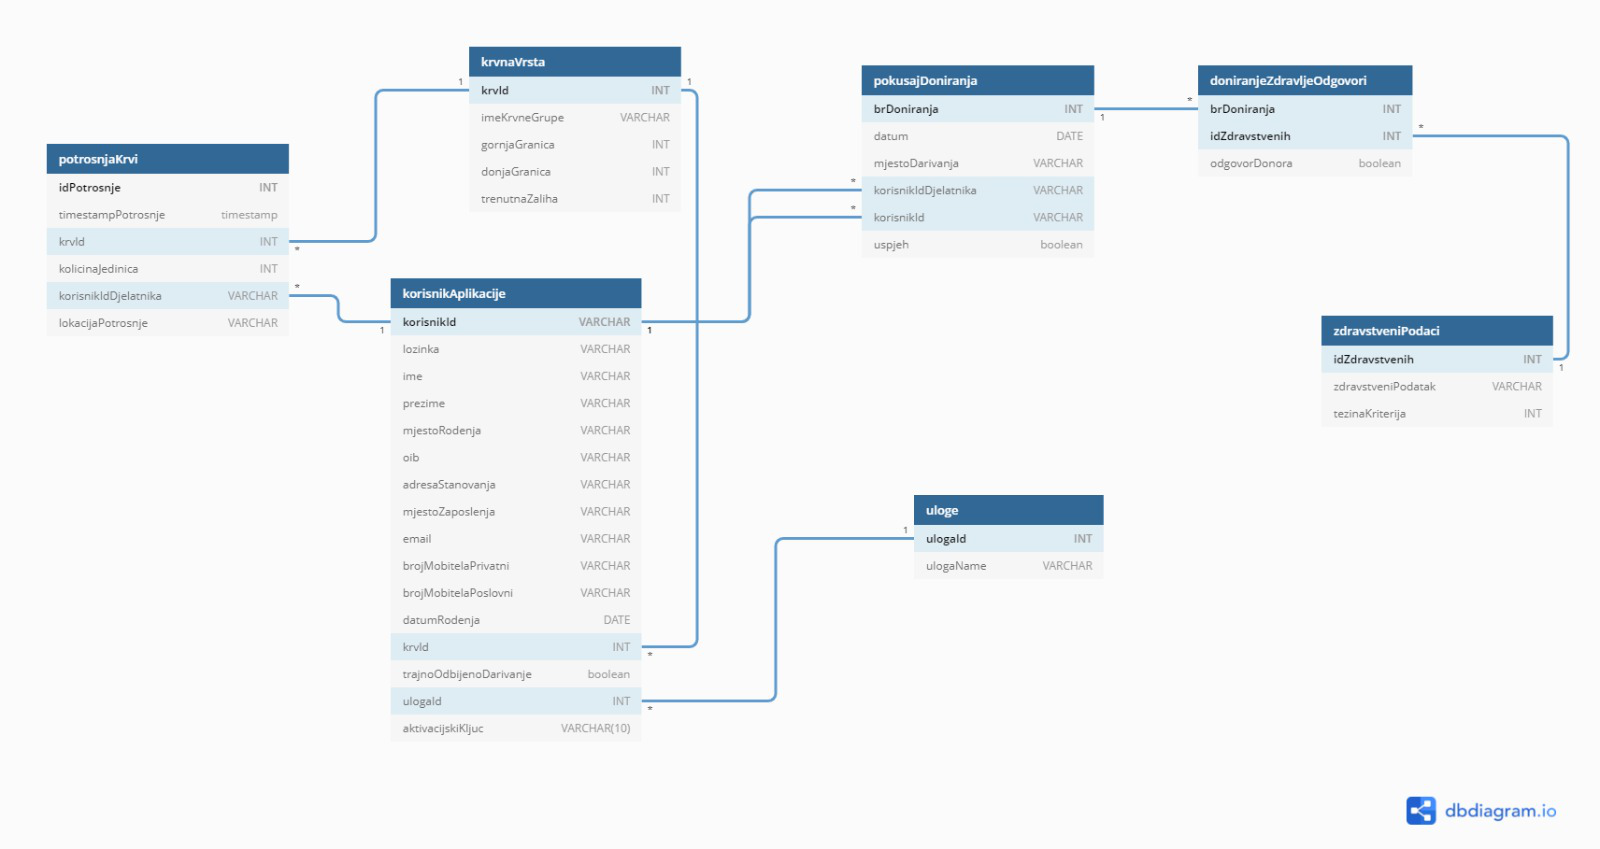
\includegraphics[width=\textwidth, scale=2.0]{dijagrami/relShema.png}
	\caption{relacijski model baze podataka}
	\label{fig:dijagram_baze}
\end{figure}
			\eject
			
		\section{Dijagram razreda}
		
<<<<<<< HEAD
	Dijagram razreda pokazuje odnose između različitih objekata, te njihove atribute i operacije kojima vladaju. Na slikama 4.5., 4.6, 4.7. prikazani su razredi koji pripadaju \textit{backend} dijelu naše arhitekture. Radi jednostavnosti, dijagram razreda je podijeljen u više slika, no bez obzira na to, prikazani razredi na neki način komuniciraju.
	Na idućoj slici prikazan je model podataka kojima backend rukuje. Korisnik aplikacije (administartor, djelatnik banke, donor) modeliran je razredom \textit{User}. Razred \textit{Blood} modelira krvne grupe. Razred \textit{Consumption} modelira potrošnju krvi. Razred \textit{Donation} modelira pokušaj donacije krvi, dok razred \textit{Role} modelira 3 moguće uloge u aplikaciji. Razred HealthData modelira zdravstvena pitanja, a HealthDataAnswered modelira odgovore na određena zdravstvena pitanja. Također navedene su enumeracije za nazive krvnih grupa i nazive uloga.
=======
	Dijagram razreda pokazuje odnose između različitih objekata, te njihove atribute i operacije kojima vladaju. Na slikama 4.5., 4.6, 4.7., 4.8 prikazani su razredi koji pripadaju \textit{backend} dijelu naše arhitekture. Radi jednostavnosti, dijagram razreda je podijeljen u više slika, no bez obzira na to, prikazani razredi na neki način komuniciraju.
	Na idućoj slici prikazan je model podataka kojima backend rukuje. Korisnik aplikacije (administartor, djelatnik banke, donor) modeliran je razredom \textit{User}. Razred \textit{Blood} modelira krvne grupe. Razred \textit{Consumption} modelira potrošnju krvi. Razred \textit{Donation} modelira pokušaj donacije krvi, dok razred \textit{Role} modelira 3 moguće uloge u aplikaciji. Razredi \textit{HealthData}, \textit{HealthDataAnswered} i \textit{HealthDataAnsweredId} modeliraju zdravstvene podatke potrebne za donacije. Također navedene su enumeracije za nazive krvnih grupa i nazive uloga.
>>>>>>> devdoc
\begin{figure}[H]
	\centering
	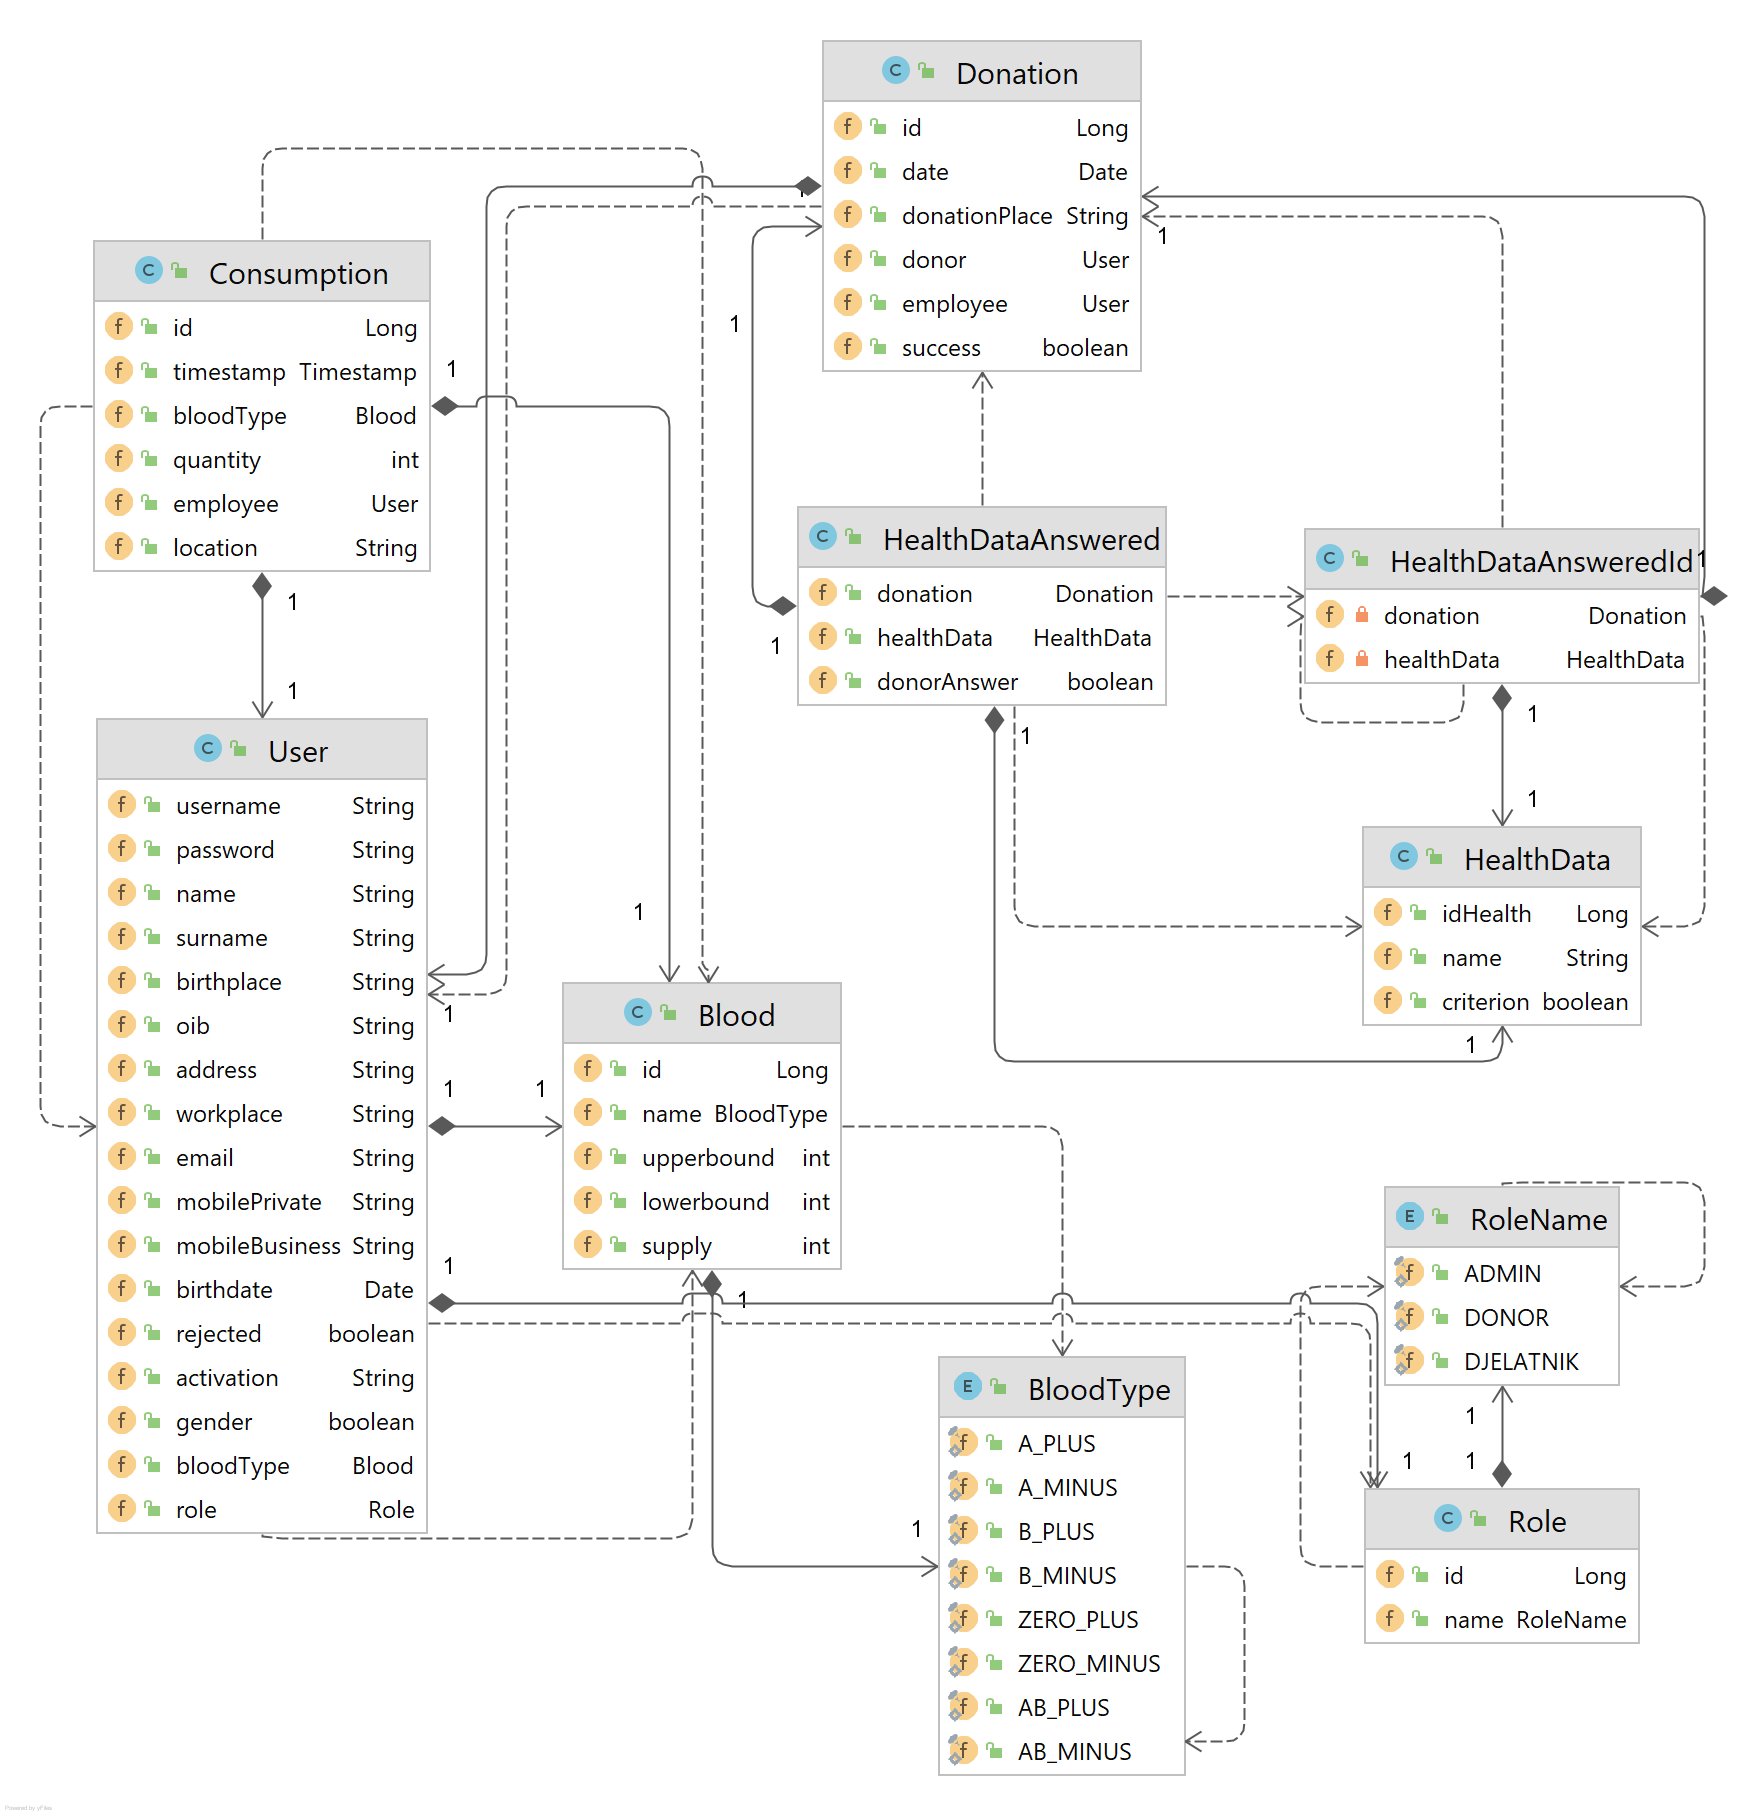
\includegraphics[width=\textwidth, scale=2.0]{dijagrami/dijagram_razreda1}
	\caption{Dijagram razreda koji opisuje model}
	\label{fig:dijagram_modela}
\end{figure}
		
	\eject
<<<<<<< HEAD
	Na idućoj slici prikazana je sloj \textit{backenda} koji je odgovoran za neposrednu komunikaciju s poslužiteljem baze podataka. Kao glavna komponenta na slici prikazano je sučelje JpaRepository, koje predstavlja apstraktni repozitorij podataka. Iz tog sučelja, izvedena su sučelja UserRepository, RoleRepository, BloodRepository, ConsumptionRepository, DonationRepository, HealthDataRepository i HealthDataAnsweredRepository. Ta sučelja predstavljaju repozitorij podataka za prije navedene razrede modela, tj. oni predstavljaju poveznicu s bazom ili DAO (eng. Data Access Object). Također koriste se različite ServiceJpa klase koje koriste te repozitorije, te one implementiraju sučelje imeKlaseService. 
=======
	Na idućoj slici prikazana je sloj \textit{backenda} koji je odgovoran za neposrednu komunikaciju s poslužiteljem baze podataka. Imamo sučelja UserRepository, RoleRepository, BloodRepository, ConsumptionRepository, DonationRepository, HealthDataRepository te HealthDataAnsweredRepository koja predstavljaju apstraktni repozitorij podataka. Ta sučelja predstavljaju repozitorij podataka za prije navedene razrede modela, tj. oni predstavljaju poveznicu s bazom ili DAO (eng. Data Access Object). Također koriste se različite Service klase koje koriste te repozitorije, te one implementiraju sučelje imeKlaseService.  
>>>>>>> devdoc
	
\begin{figure}[H]
	\centering
	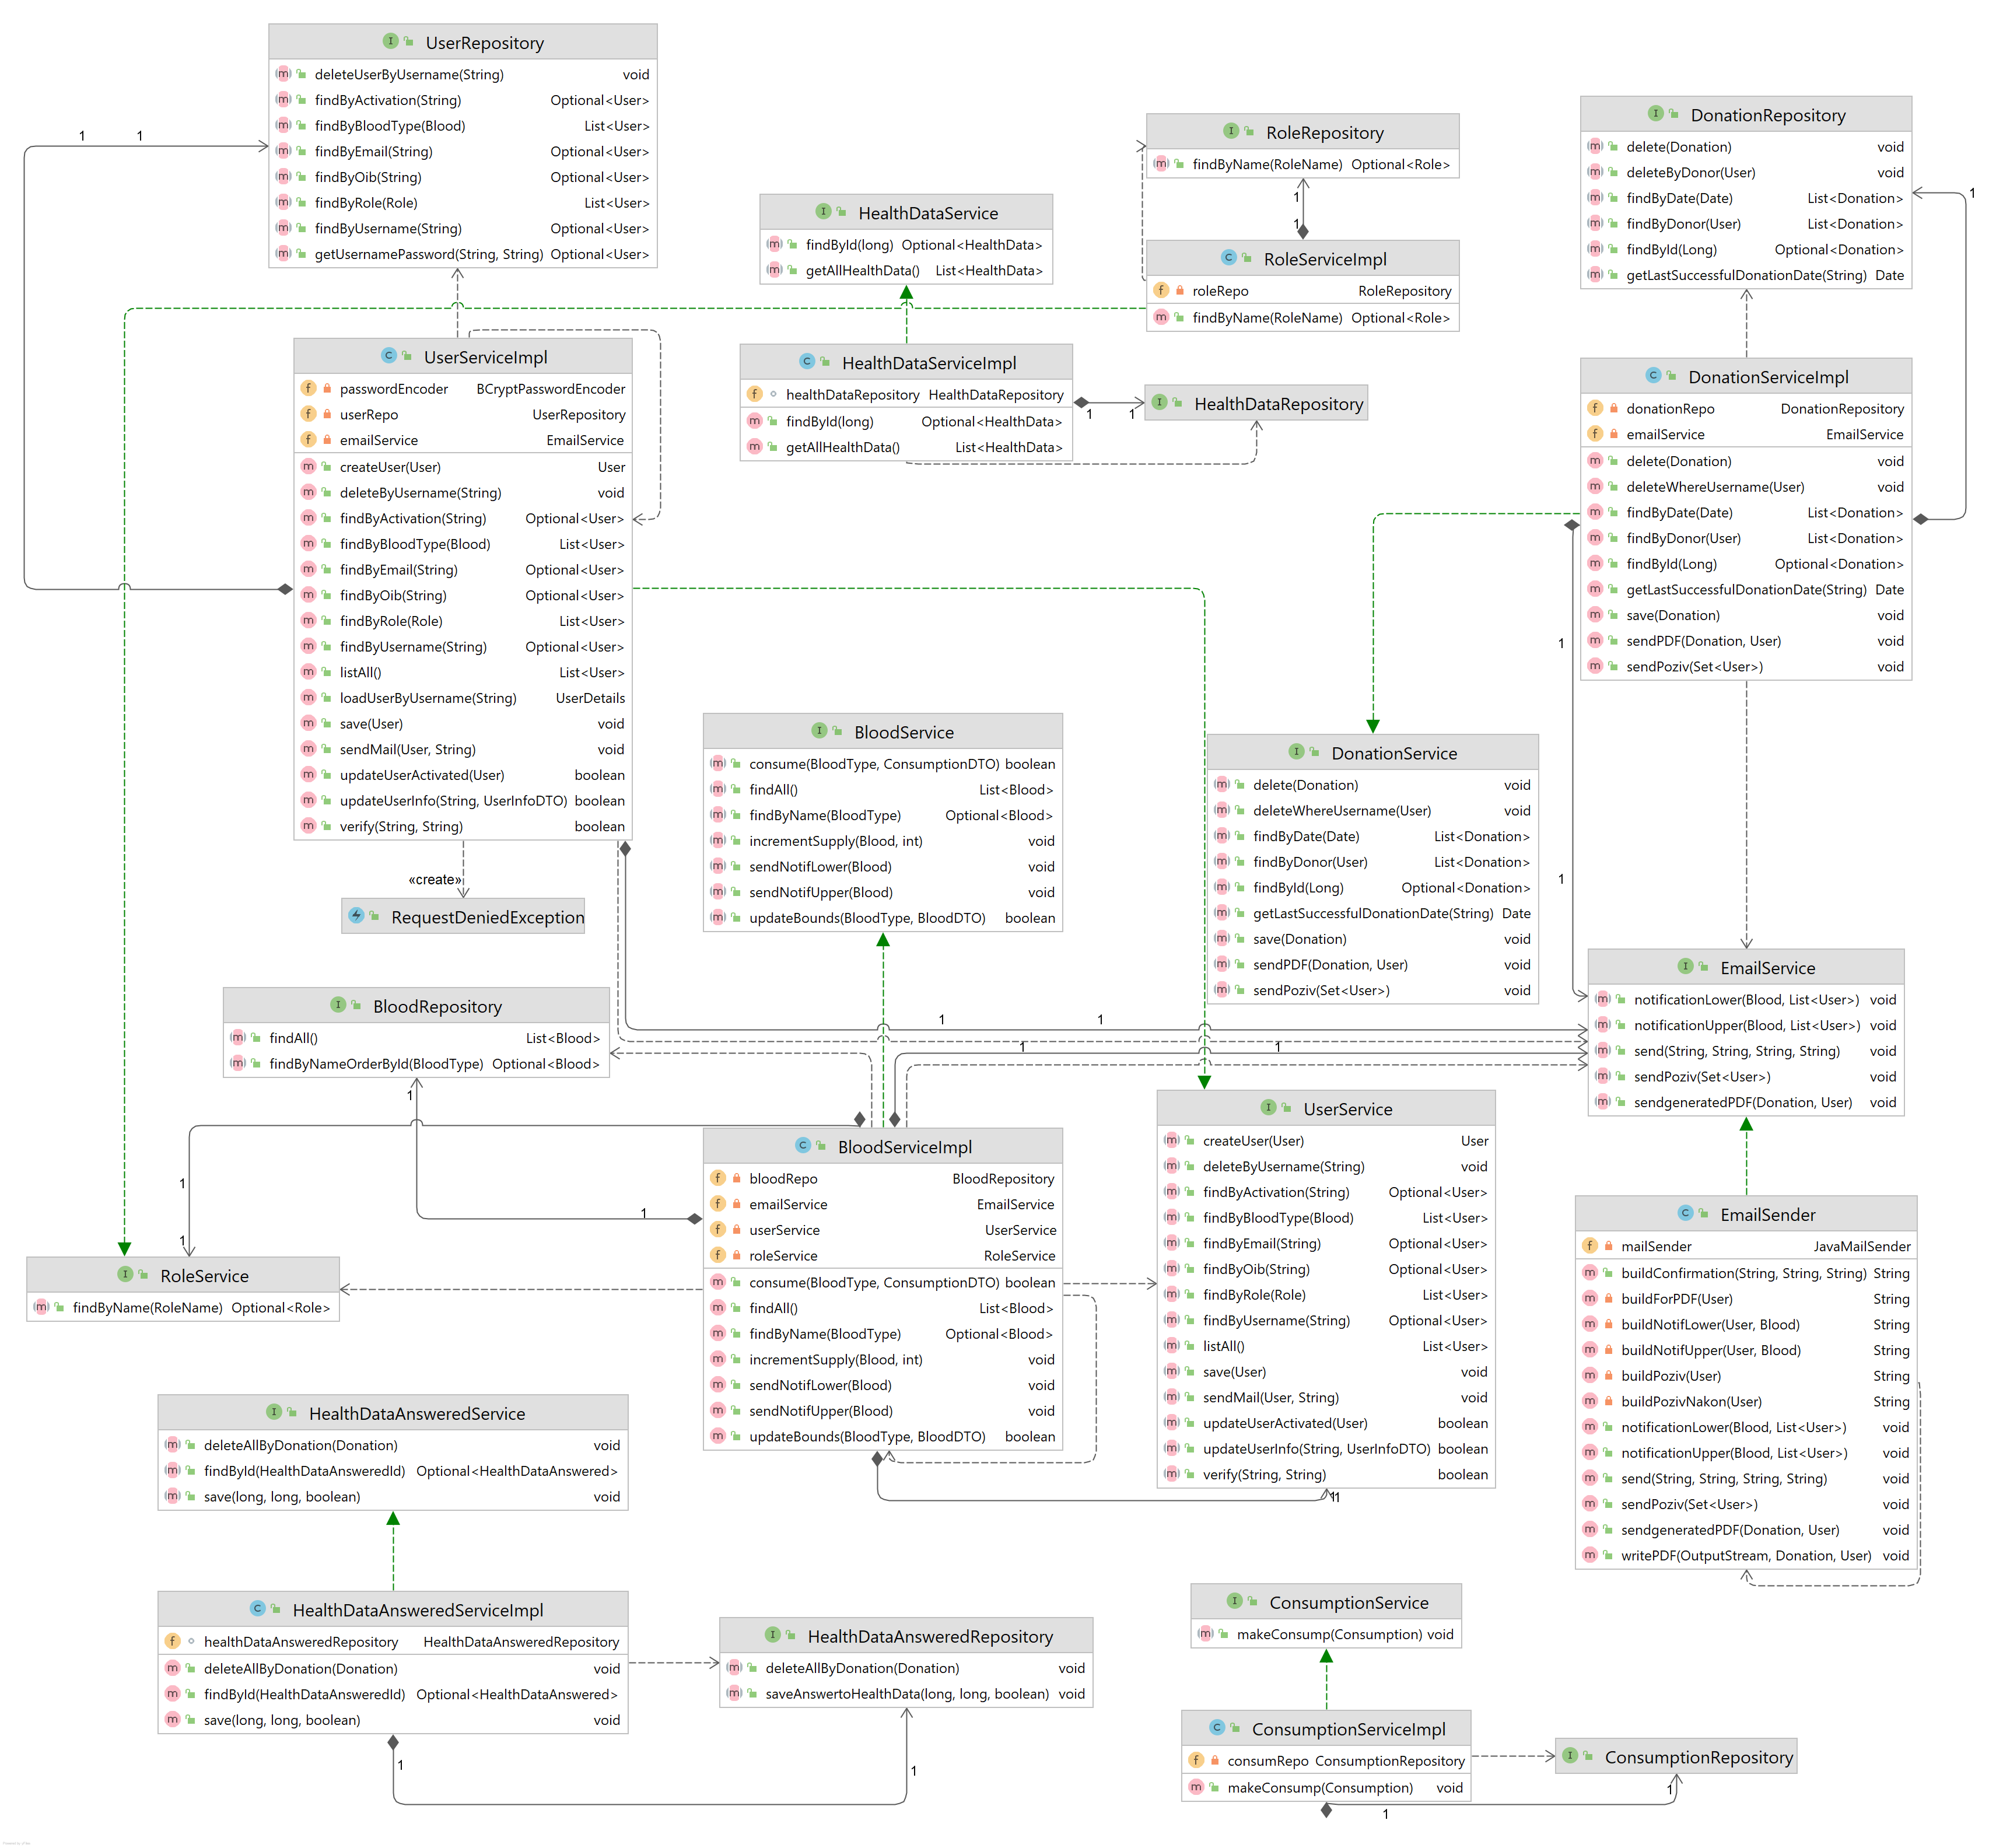
\includegraphics[width=\textwidth, scale=2.0]{dijagrami/dijagram_razreda2}
	\caption{Dijagram razreda koji opisuju repozitorije}
	\label{fig:dijagram_repozitorija}
\end{figure}

\eject

	Na zadnje dvije slike prikazani su \textit{Controlleri} koji komuniciraju s vanjskim svijetom odnosno \textit{frontendom} te upravljaju modelom podataka i DTO-ovi (eng. Data Transfer Object) koje oni koriste za prijenos podataka. Ovdje vidimo razrede UserController, RoleController, BloodController, ConsumptionController, DonationController, AdminController i HealthDataController. Svi ti razredi koriste Java anotaciju RestController koji predstavlja REST endpoint i DTO-ove koji su u paketu \textit{Util}. Ti razredi su oni koji dobivaju zahtjeve iz vanjskog svijeta, a odgovaraju HTTP odgovorima i JSON objektima.

	
\begin{figure}[H]
	\centering
	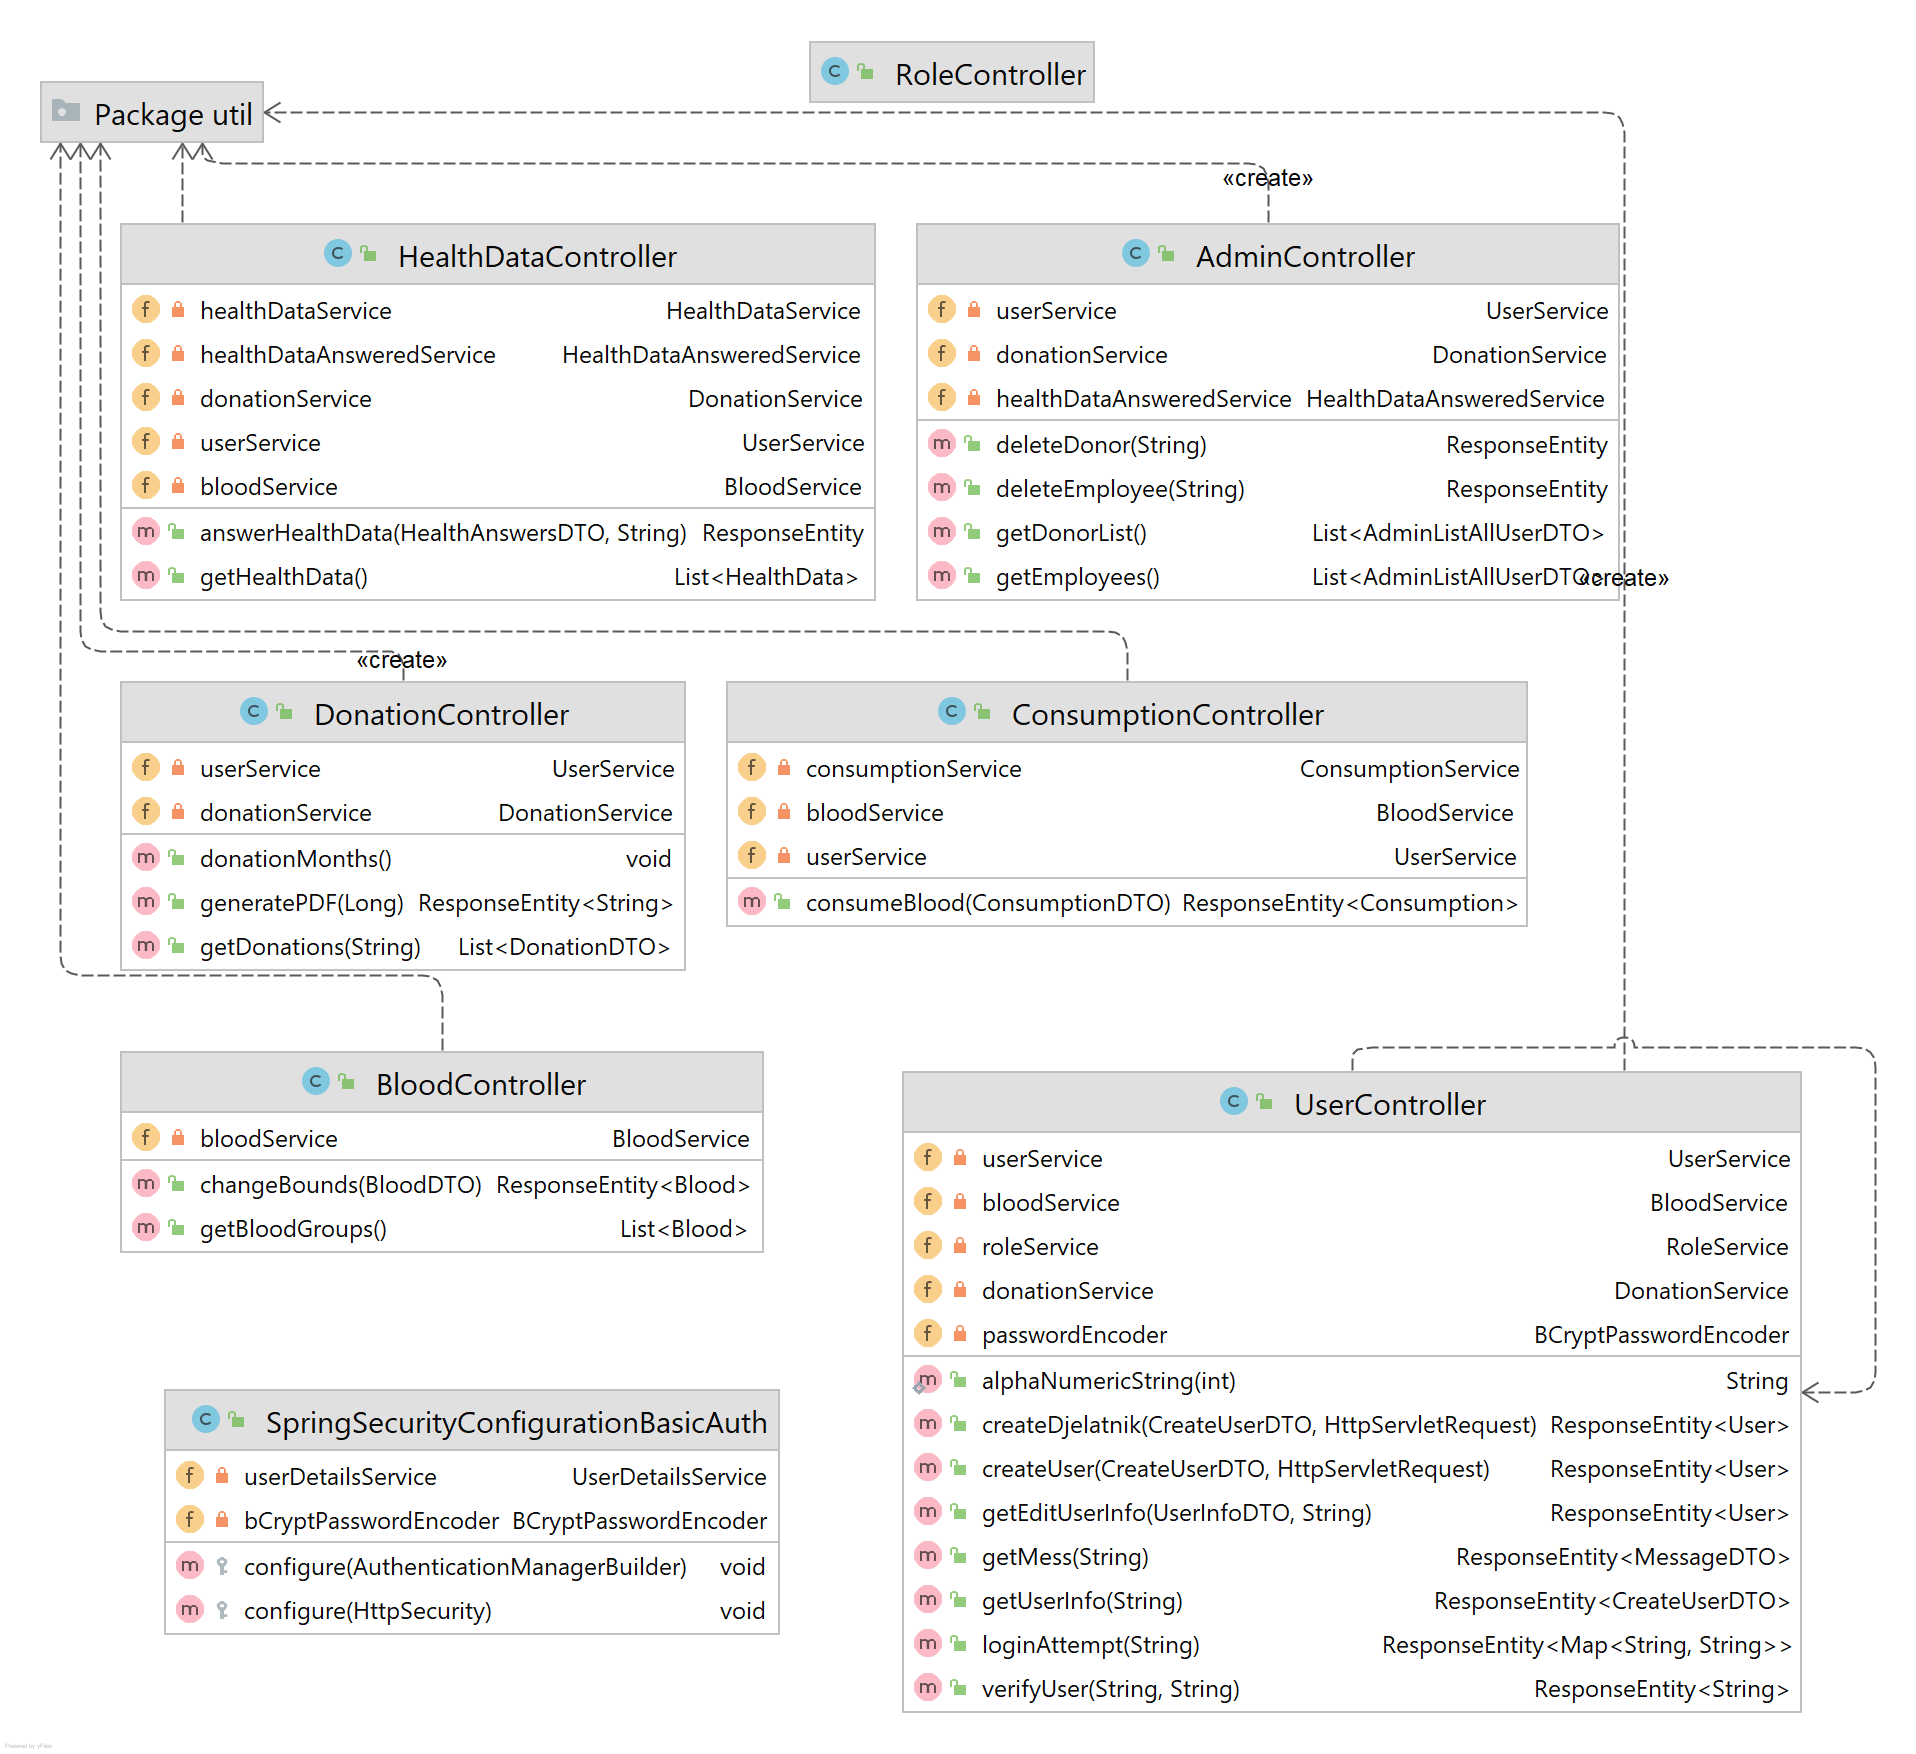
\includegraphics[width=\textwidth, scale=0.5]{dijagrami/dijagram_razreda3}
	\caption{Dijagram razreda koji opisuju kontrolere}
	\label{fig:dijagram_kontrolera}
\end{figure}

\begin{figure}[H]
	\centering
	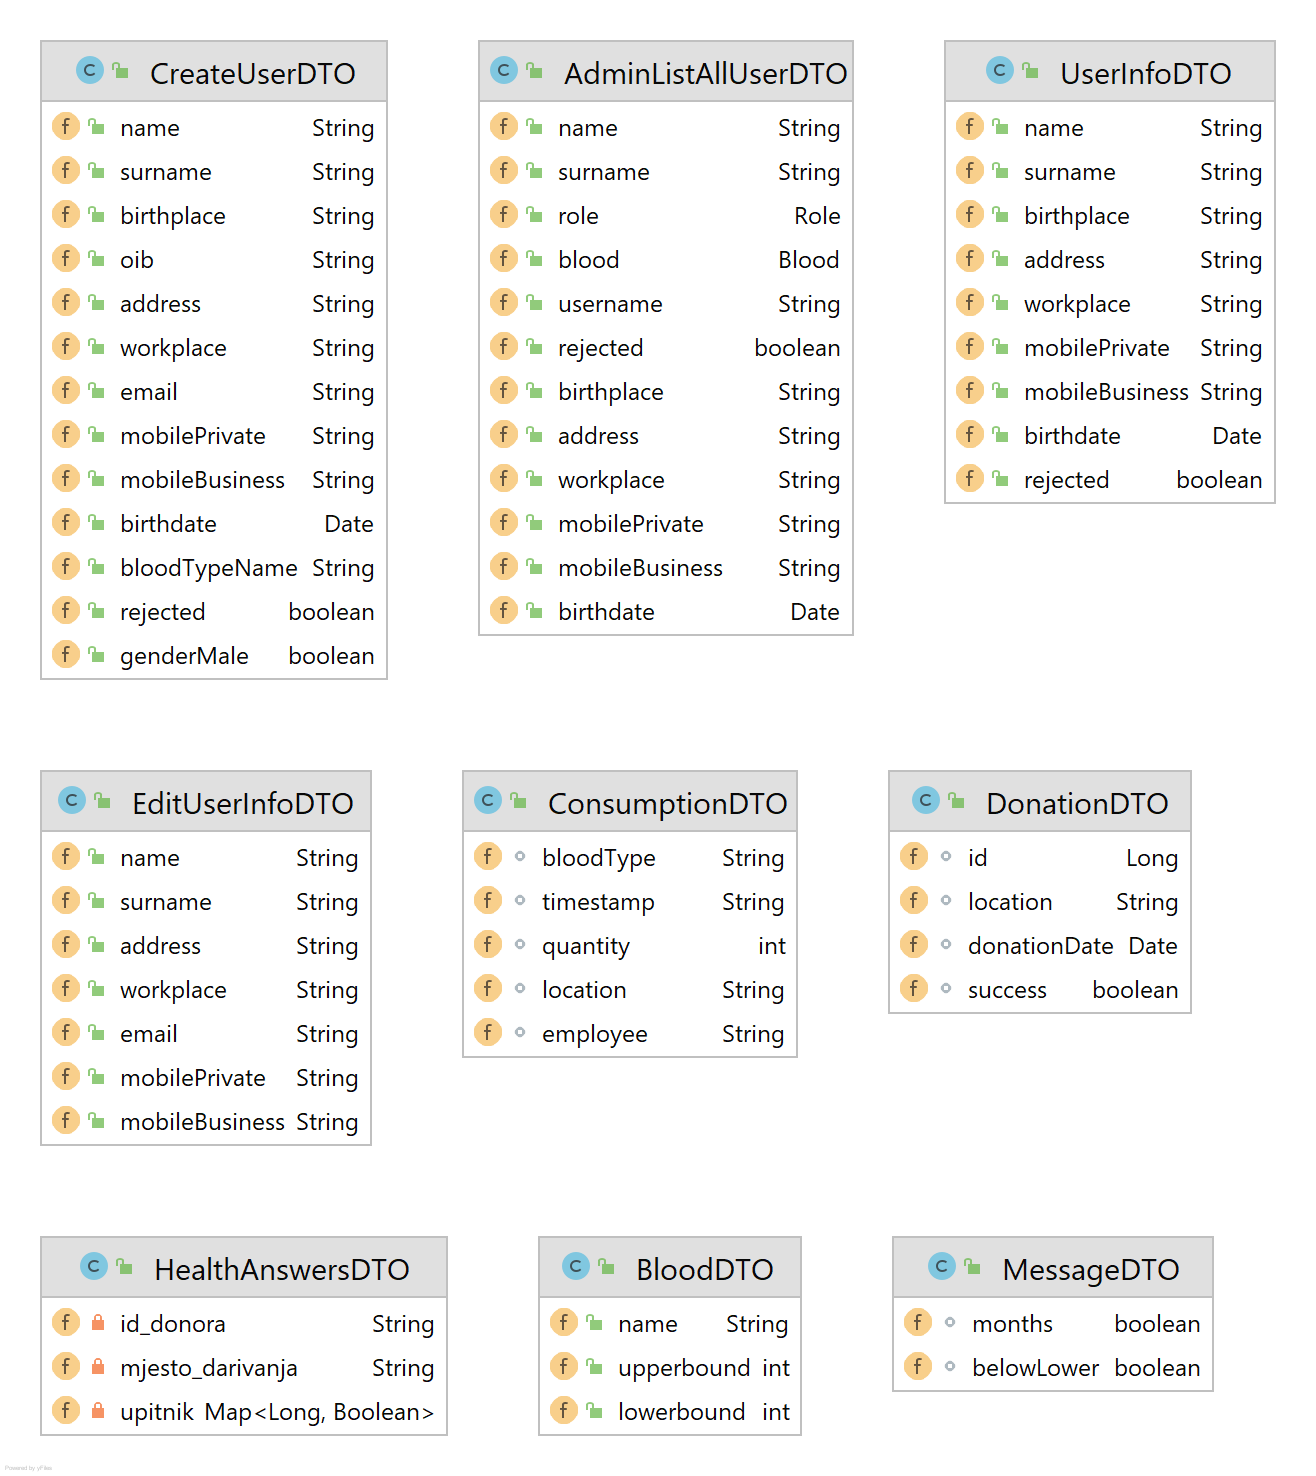
\includegraphics[width=\textwidth, scale=0.5]{dijagrami/dijagram_razreda4}
	\caption{Dijagram razreda koji opisuju DTO-ove}
	\label{fig:dijagram_DTO}
\end{figure}

\eject
			
			
		
		\section{Dijagram stanja}
			Dijagram stanja primijenjuje se za opis stanja objekta i za opisivanje prijelaza iz jednog u drugo stanje. Priložena slika prikazuje stanjadijagram stanja za registriranog donora. Početno stanje je početna stranica aplikacije. U izborniku aplikacije donor može odabrati jednu od mogućnosti. Klikom na "Moji podaci" prikazuju mu se njegovi podaci, koje moeže urediti. Odabirom opcije "Poruke" prikazuju se poruke donoru koje mu javlja sustav. Klikom na 
"Povijest darivanja" prikazuju se prijašnja darivanja za koje, ako je darivanje uspješno,  može izvaditi PDF potvrdu.

\begin{figure}[H]
	\centering
	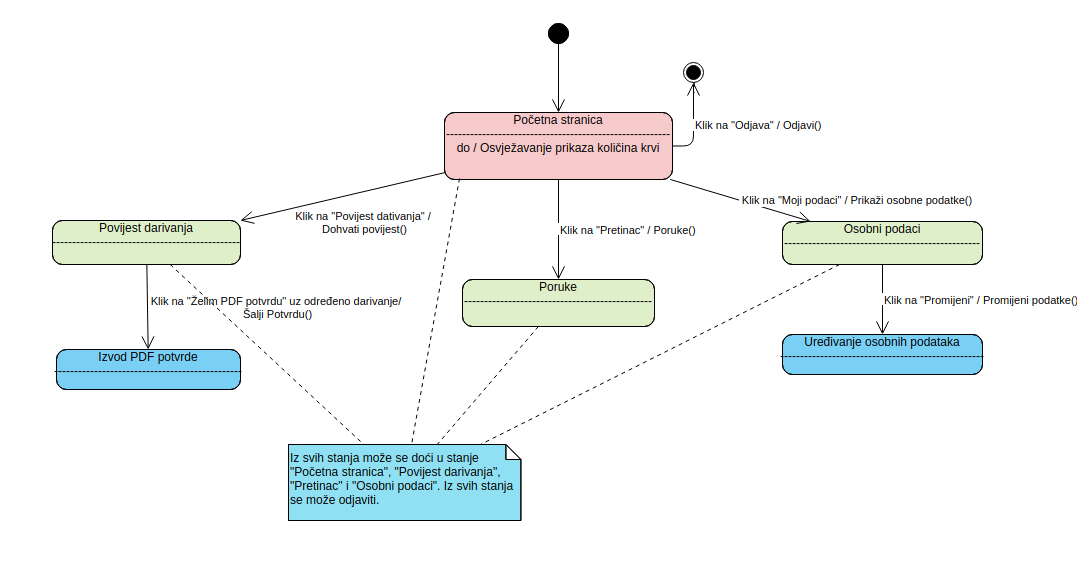
\includegraphics[width=\textwidth, scale=0.7]{dijagrami/dijagram_stanja}
	\caption{Dijagram stanja}
	\label{fig:dijagram_stanja}
\end{figure}
			
			
			
			
			\eject 
		
		\section{Dijagram aktivnosti}
			Dijagram aktivnosti prikazuje povezane aktivnosti na visokoj apstrakcijskoj razini,odnosno intuitivno prikazuje kako podaci teku kroz aplikaciju i kako se
kontrola nad podacima mijenja. U modeliranju toka upravljanja svaki novi korak poduzima se nakon završenog prethodnog. Idući dijagram prikazuje proces smanjivanja količine krvi slanjem u zdravstvenu ustanovu. Ovaj proces može provesti djelatnik banke. Proces započinje prijavom, djelatnik banke odabere krvnu grupu na prikazu količina krvi i unese količinu krvi koju želi poslati zdravstvenoj ustanovi. Kada transakcija završi prikazuje mu se potvrda o smanjenju krvi.
		
\begin{figure}[H]
	\centering
	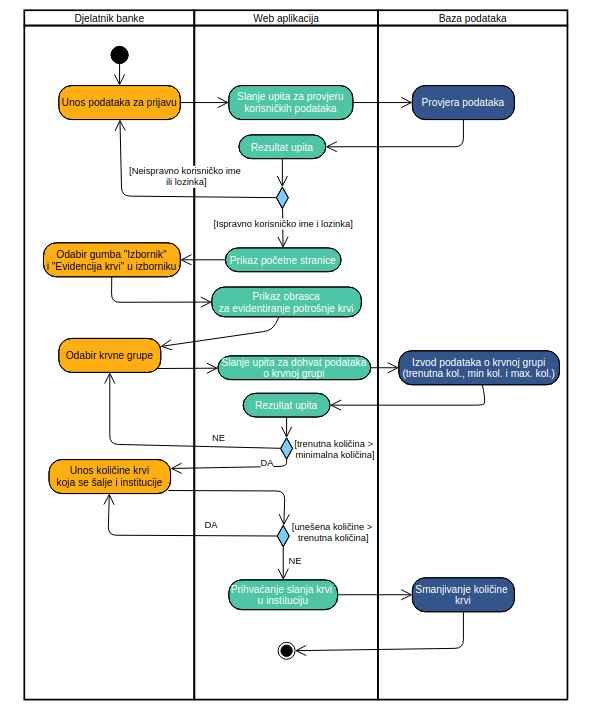
\includegraphics[width=\textwidth, scale=0.5]{dijagrami/dijagram_aktivnosti}
	\caption{Dijagram aktivnosti}
	\label{fig:dijagram_aktivnosti}
\end{figure}
				
			
			\eject
		\section{Dijagram komponenti}
		
			Dijagram komponenti omogućuje nam pogled na sustav s visoke razine apstrak-
cije. Web aplikacija komunicira sa sustavom preko dva sučelja. Prvo sučelje služi
za dohvat samih stranica, dakle HTML, CSS i JS datoteka. Drugo sučelje služi
za komunikaciju između aplikacije i baze podataka. Dakle, web aplikacija šalje
zahtjev REST API-u, koji preko kontrolera komunicira s repozitorijima
podataka, koji predstavljaju sloj povezanosti između baze podataka i kontrolera.  Podaci koji su pristigli
iz baze se šalju dalje MVC arhitekturi u obliku DTO (Data transfer object).
React view komponenta preko dostupnih sučelja komunicira s web aplikacijom te ovisno o korisnikovim akcijama osvježava prikaz i dohvaća nove podatke ili datoteke.

\begin{figure}[H]
	\centering
	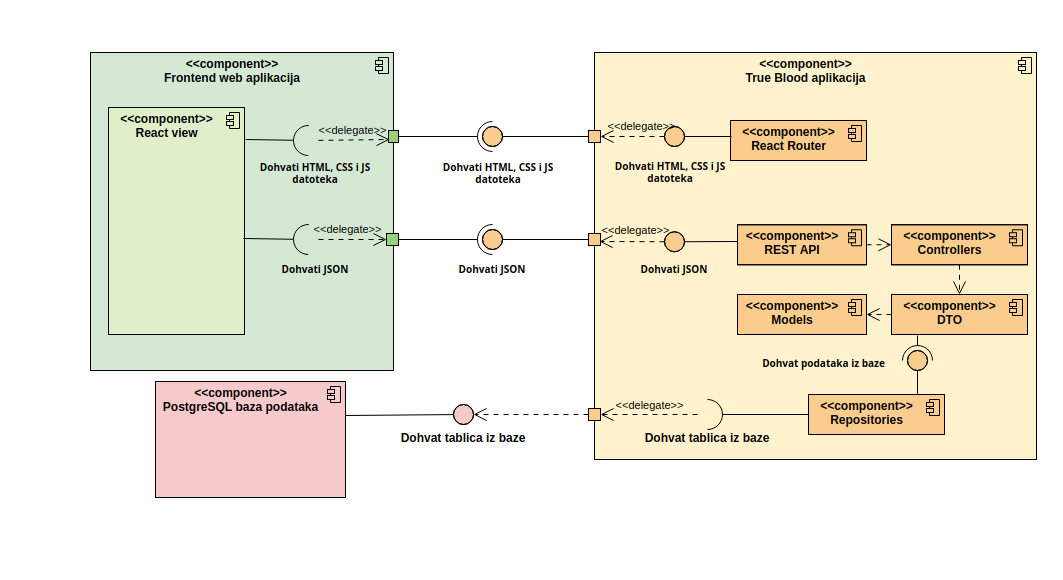
\includegraphics[width=\textwidth, scale=0.5]{dijagrami/dijagram_komponenti}
	\caption{Dijagram komponenti}
	\label{fig:dijagram_komponenti}
\end{figure}

	\chapter{Implementacija i korisničko sučelje}
		
		
		\section{Korištene tehnologije i alati}
		
			Komunikacija u timu realizirana je korištenjem platforme \underline{Whatsapp}\footnote{\url{https://www.whatsapp.com/}}. 
			Za izradu UML dijagrama korišten je alat \underline{Astah Professional}\footnote{\url{https://astah.net/products/astah-professional/}} i \underline{Visual Paradigm}\footnote{\url{https://online.visual-paradigm.com/}}, a kao sustav za upravljanje izvornim kodom \underline{Git}\footnote{\url{https://git-scm.com/}}. 
			Udaljeni repozitorij projekta je dostupan na web platformi \underline{GitLab}\footnote{\url{https://gitlab.com/}}.
			\par
			Kao razvojno okruženje korišten je \underline{IntelliJ IDEA}\footnote{\url{https://www.jetbrains.com/idea/}} - integrirano razvojno okruženje (IDE) tvrtke JetBrains i \underline{Eclipse}\footnote{\url{https://www.eclipse.org/ide/}}. 
            \par
            Aplikacija je napisana u \underline{Javi}\footnote{\url{https://www.java.com/en/}} koristeći ekosustav \underline{Java Spring}\footnote{\url{https://spring.io/}} za
            izradu backenda te \underline{React}\footnote{\url{https://reactjs.org/}} i jezik \underline{JavaScript}\footnote{\url{https://www.javascript.com/}} za izradu frontenda. 
            \par
            Baza podataka koju smo koristili je (\underline{PostgreSQL}\footnote{\url{https://www.postgresql.org/}}) i ona se nalazi na \underline{pgAdmin}\footnote{\url{https://www.pgadmin.org/}}.

            
            \vspace*{\fill}

			
			
			\eject 
		
	
		\section{Ispitivanje programskog rješenja}
			
Nakon što smo završili s izradom testirali smo rad aplikacije koristeći JUnit tehnologiju i Selenium WebDriver. Testovi su dali zadovoljavajuće rezultate te možemo zaključiti da smo uspjeli implementirati zadane funkcionalnosti.
			
			\subsection{Ispitivanje komponenti}
			
Za ispitivanje komponenti koristili smo JUnit tehnologiju. JUnit okvir je za testiranje komponenti sustava programiranog u Javi. Ispitali smo funkcionalnosti ažuriranja osobnih podataka donora, promjenu optimalnih granica krvi i evidencije krvi slanjem u instituciju. Koriste se objekti tipa UserContoller, BloodController i ConsumptionController na kojima se pozivaju ispitivane funkcionalnosti te UserService, BloodService i RoleService koji su potrebni za dohvaćanje podataka korištenih u funkcijama.
\\\\
\textbf{Ažuriranje osobnih podataka donora}
\\\\
Pozivom funkcije getEditUserInfo iz klase UserController želimo donoru uspješno promijeniti prezime. Na kraju uspoređujemo je li prezime ažuriranog donora jednako željenom novom prezimenu.

\begin{figure}[H]
	\centering
	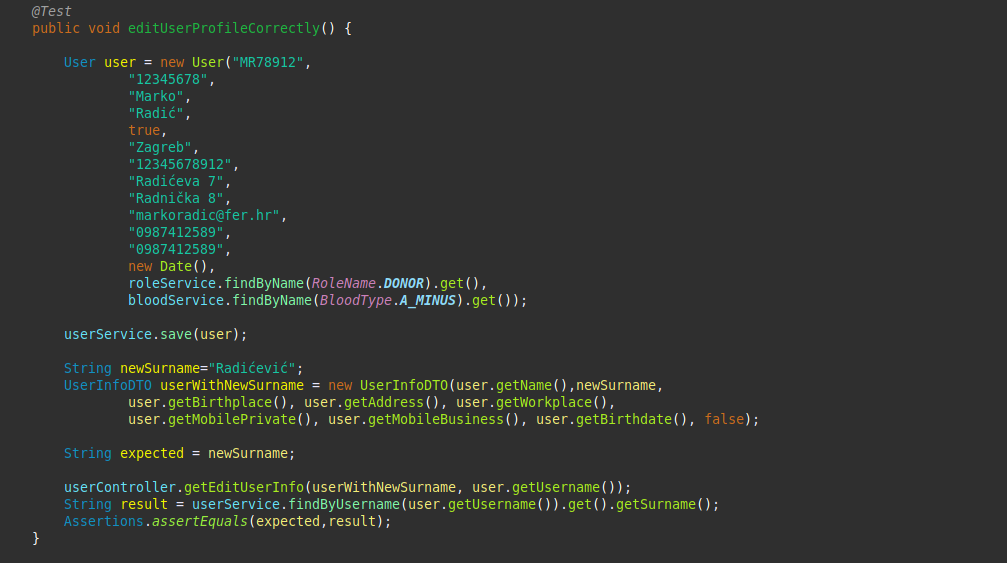
\includegraphics[width=\textwidth, scale=0.5]{slike/unit1}
	\caption{Unit test1}
\end{figure}
{U idućem testu pozivom iste funkcije želimo neuspješno ažurirati polje rejected, koje se ne bi smjelo mijenjati. Na kraju uspoređujemo je li dobivena statusna poruka jednaka očekivanoj "400 BADREQUEST" što bi značilo da aplikacija na pobuđenu situaciju prikladno odgovara.}
\begin{figure}[H]
	\centering
	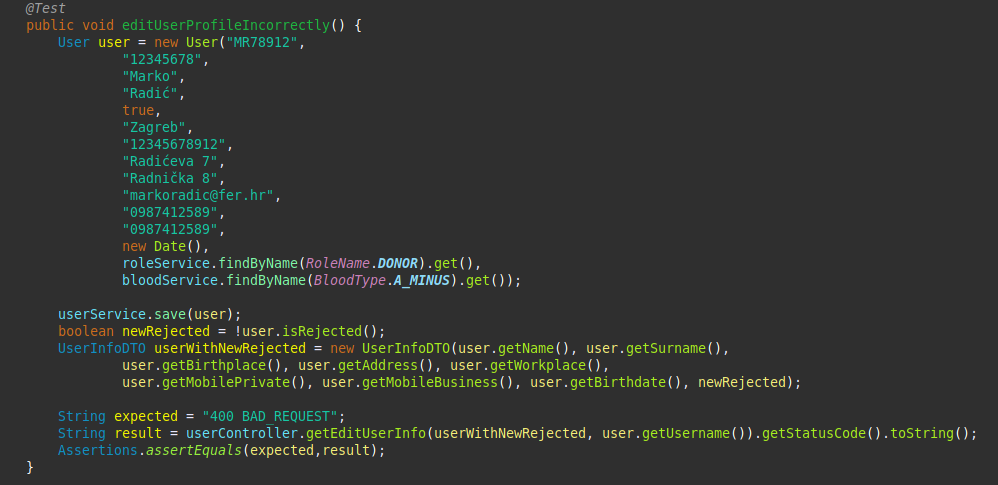
\includegraphics[width=\textwidth, scale=0.5]{slike/unit2}
	\caption{Unit test2}
\end{figure}
\textbf{Promjena optimalnih granica krvi}
\\\\
Pozivom funkcije changeBounds iz klase BloodController želimo uspješno promijeniti donju optimalnu granicu određene krvne grupe. Na kraju uspoređujemo je li donja optimalna granica ažurirane krvne grupe jednaka željenoj granici.
\begin{figure}[H]
	\centering
	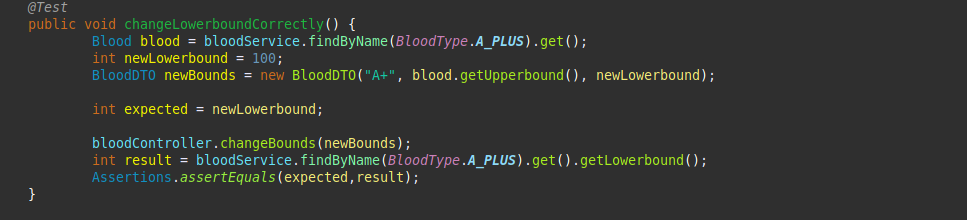
\includegraphics[width=\textwidth, scale=0.5]{slike/unit3}
	\caption{Unit test3}
\end{figure}
\eject
{U idućem testu pozivom iste funkcije želimo neuspješno ažurirati donju optimalnu granicu, koja bi uvijek morala biti pozitivna. Na kraju uspoređujemo je li dobivena statusna poruka jednaka očekivanoj "400 BADREQUEST" što bi značilo da aplikacija na pobuđenu situaciju prikladno odgovara.}
\begin{figure}[H]
	\centering
	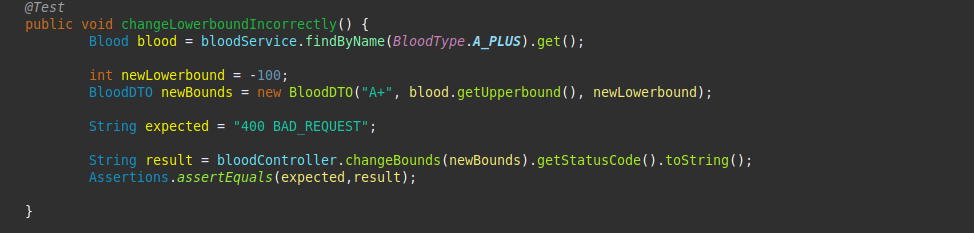
\includegraphics[width=\textwidth, scale=0.5]{slike/unit4}
	\caption{Unit test4}
\end{figure}
\textbf{Evidencija krvi slanjem u instituciju}
\\\\
Pozivom funkcije consumeBlood iz klase ConsumptionController želimo uspješno evidentirati slanje određene krvne grupe u neku instituciju. Na kraju uspoređujemo je li trenutna količina ažurirane krvne grupe jednaka količini umanjenjoj za količinu koja je poslana u instituciju.
\begin{figure}[H]
	\centering
	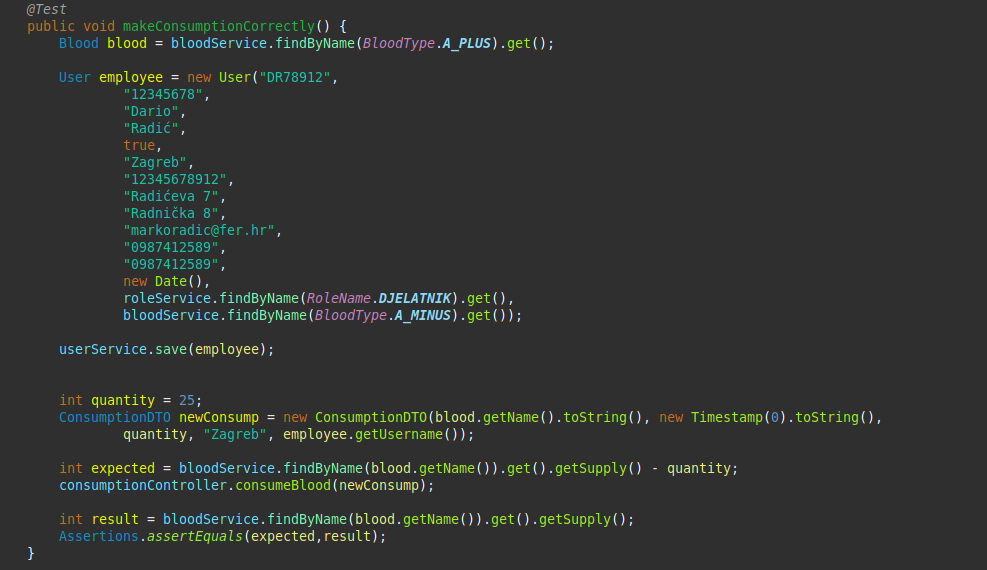
\includegraphics[width=\textwidth, scale=0.5]{slike/unit5}
	\caption{Unit test5}
\end{figure}
\eject	
{U idućem testu pozivom iste funkcije želimo neuspješno evidentirati slanje krvi, čija bi količina uvijek morala biti pozitivna i veća od 0. Na kraju uspoređujemo je li dobivena statusna poruka jednaka očekivanoj "400 BADREQUEST" što bi značilo da aplikacija na pobuđenu situaciju prikladno odgovara. }
\begin{figure}[H]
	\centering
	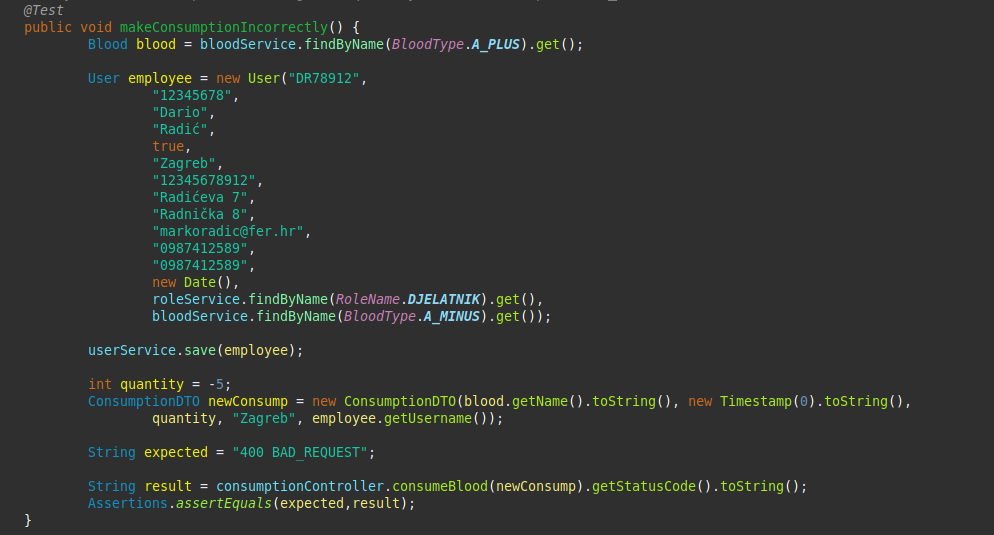
\includegraphics[width=\textwidth, scale=0.5]{slike/unit6}
	\caption{Unit test6}
\end{figure}

\begin{figure}[H]
	\centering
	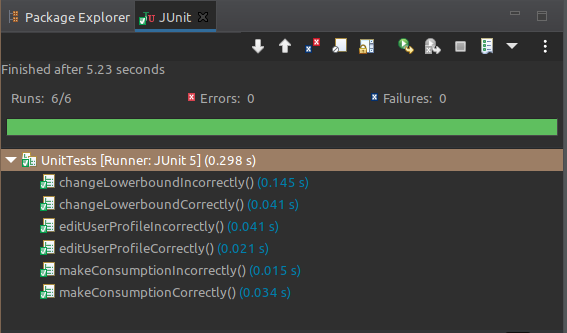
\includegraphics[width=\textwidth, scale=0.5]{slike/unit_testing}
	\caption{Rezultati ispitivanja komponenti}
\end{figure}
\eject
			
			\subsection{Ispitivanje sustava}
			Selenium WebDriver, okvir koji omogućuje programsku interakciju sa internetskim preglednicima, je bio korišten za ispitivanje sustava. Testovi su provedeni na Google Chrome pregledniku. Za sljedeće funkcionalnosti je napravljeno programsko ispitivanje:
			
			 \begin{itemize}
			 	\item {prijava (za donore, djelatnike i admin-a)}
			 	\item {promjene optimalnih granica krvnih grupa (funkcionalnost admin-a)}
			 	\item {evidencija potrošnje krvi (funkcionalnost djelatnika)}
			 	\item {upisivanje donacije u registar (funkcionalnost djelatnika)}
			 	
			 \end{itemize}
		 Korištena je dodatna funkcija za usporavanje sustava, kako se ne bi određeni dijelovi programskog koda za testiranje prerano izvršili:	
\begin{figure}[H]
	\centering
	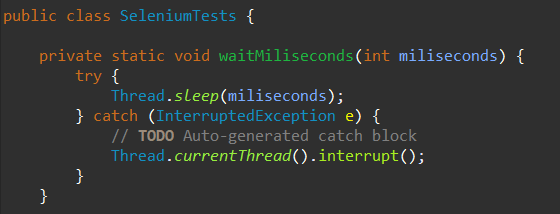
\includegraphics[width=\textwidth, scale=0.5]{slike/wait}
	\caption{Funkcija za usporavanje sustava}
\end{figure}
\eject
\textbf{Prijava}	
\\\\
Ovaj test ima za zadaću ispitati može li se svaka vrsta korisnika sustava ulogirati. Program učitava stranicu i pokušava se ulogirati sa zadanim username­-om i password­-om, te provjera je li doista ulogiran profil za zadani role. Uspjehom se smatra kada je zadani role upisan u drugo polje s desna u gornjoj traci.
\begin{figure}[H]
	\centering
	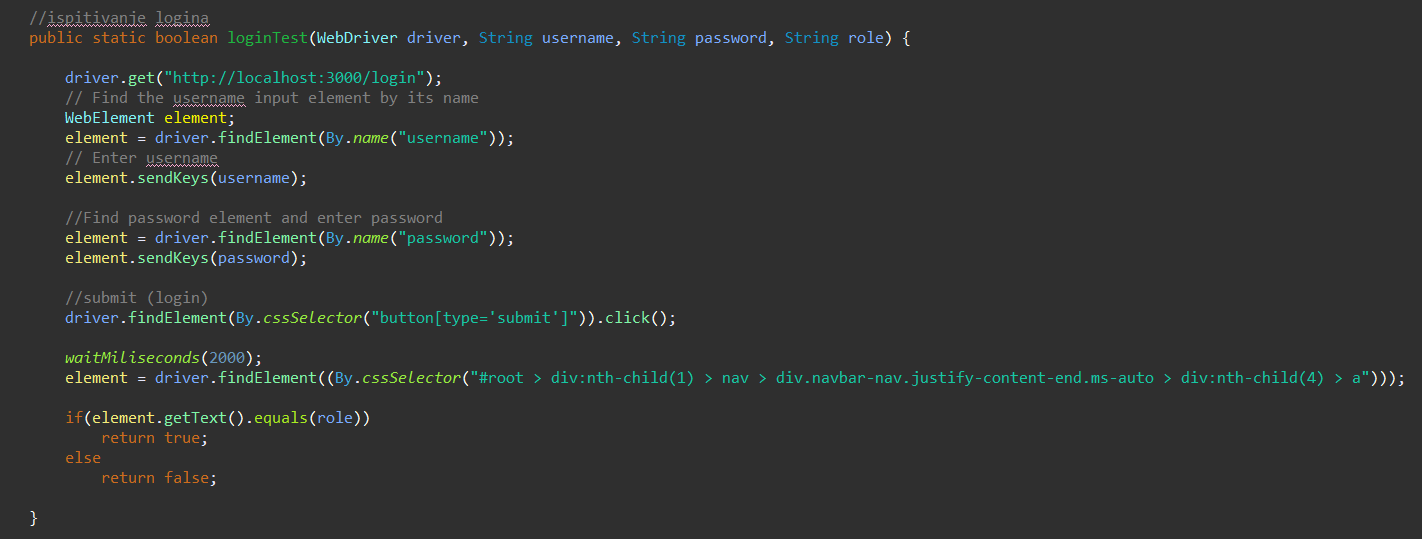
\includegraphics[width=\textwidth, scale=0.5]{slike/selenium1}
	\caption{Selenium test1}
\end{figure}

\textbf{Promjena optimalnih granica krvnih grupa}	
\\\\
Ovaj test ima za zadaću ispitati može li admin postaviti gornju i donju granicu količine krvi određene grupe, koje ako budu pređene dolazi do već spominjanih akcija. Test proglašavamo uspješnim ako poslije pritiska gumba brojevi prikazani u poljima "Gornja" i "Donja" odgovaraju željenima, ako su željene granice pozitivne vrijednosti. Ako pak nisu, onda je test uspješan kada se ispod gumba "Promjeni granice" prikaže poruka "Granice moraju biti pozitivne!".
\eject
\begin{figure}[H]
	\centering
	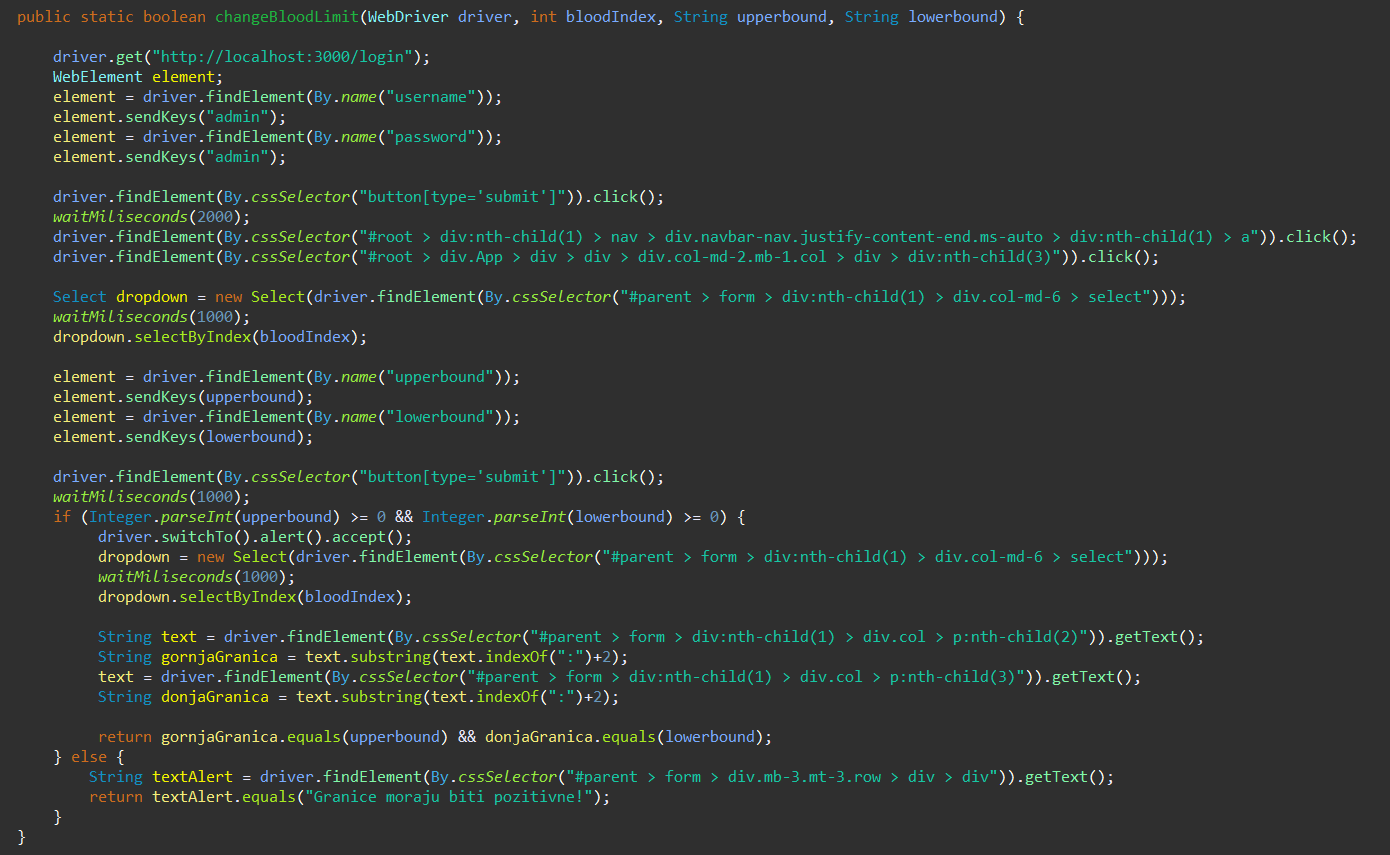
\includegraphics[width=\textwidth, scale=0.5]{slike/selenium2}
	\caption{Selenium test2}
\end{figure}

\textbf{Evidencija potrošnje krvi}	
\\\\
U ovom se testu ispituje može li djelatnik evidentirati slanje krvi u određenu instituciju i odgovara li količina određene krvne grupe u banci nakon slanja očekivanoj količini. Test je uspješan ako je količina krvi određene krvne poslije slanja jednaka očekivanoj. Krv se šalje fiktivnoj lokaciji TESTNA LOKACIJA.
\begin{figure}[H]
	\centering
	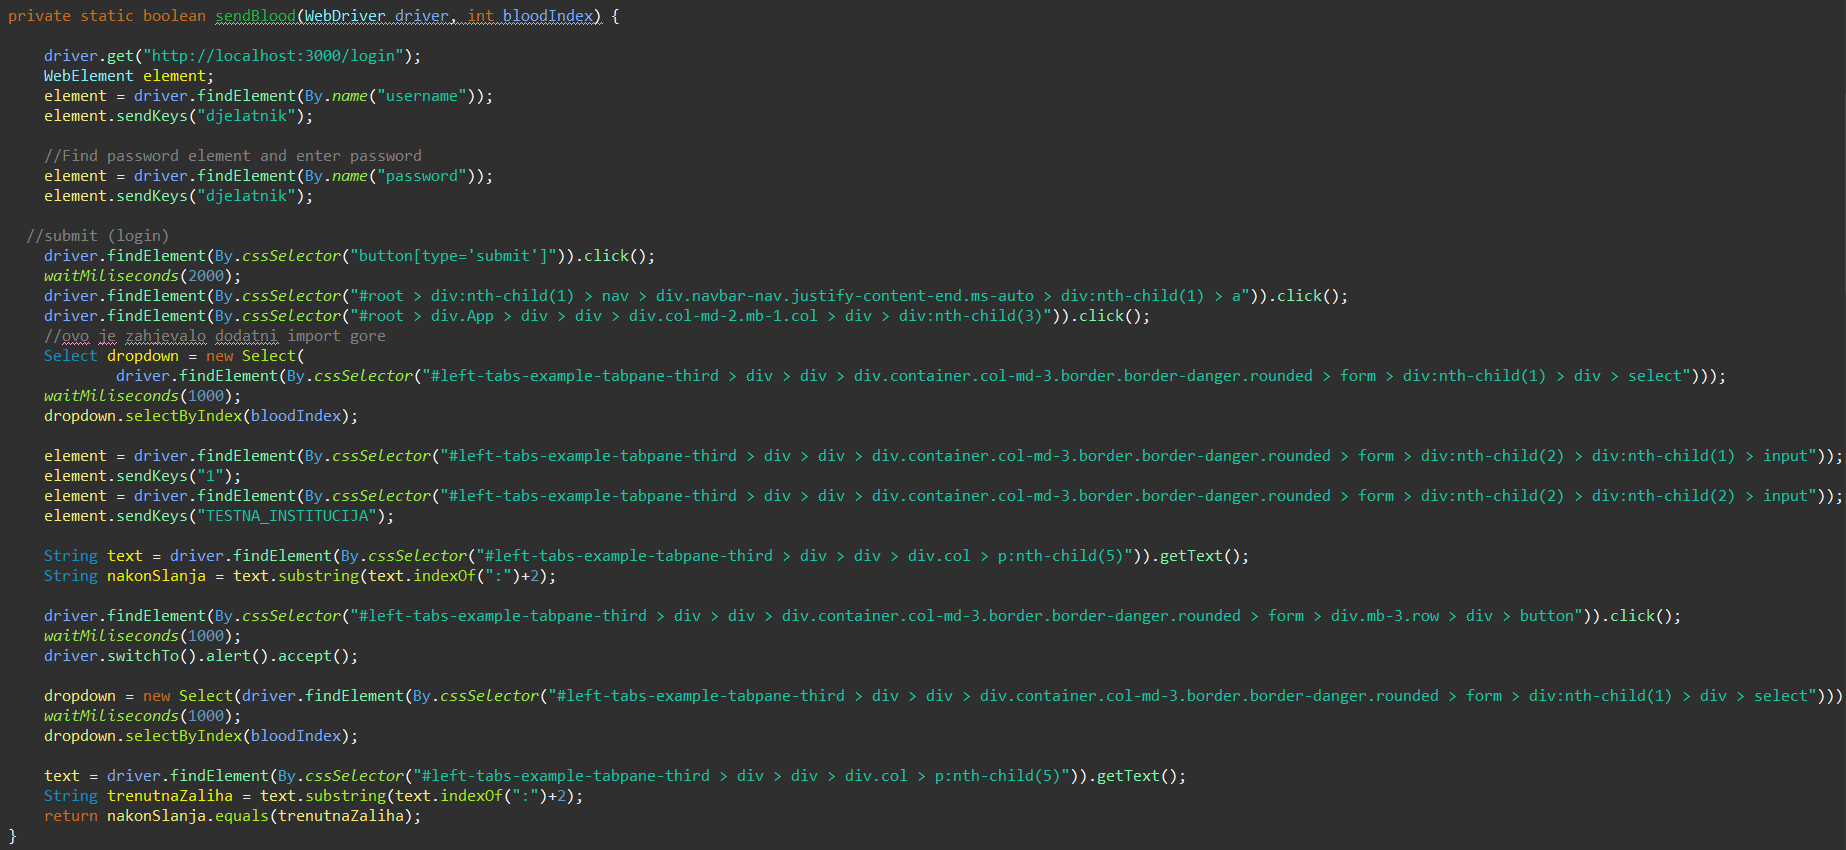
\includegraphics[width=\textwidth, scale=0.5]{slike/selenium3}
	\caption{Selenium test3}
\end{figure}
\eject
\textbf{Upisivanje donacije u registar}	
\\\\
U ovom se testu ispituje može li djelatnik evidentirati obavljenu donaciju (koju je figurativno obavio donor imena TESTDONORNAME na lokaciji TESTLOKACIJA).
Test je prolazan ako preglednik izbaci poruku "Donacija evidentirana" ili "Nije moguće donirati! Nije prošlo dovoljno vremena od zadnje donacije!".
\begin{figure}[H]
	\centering
	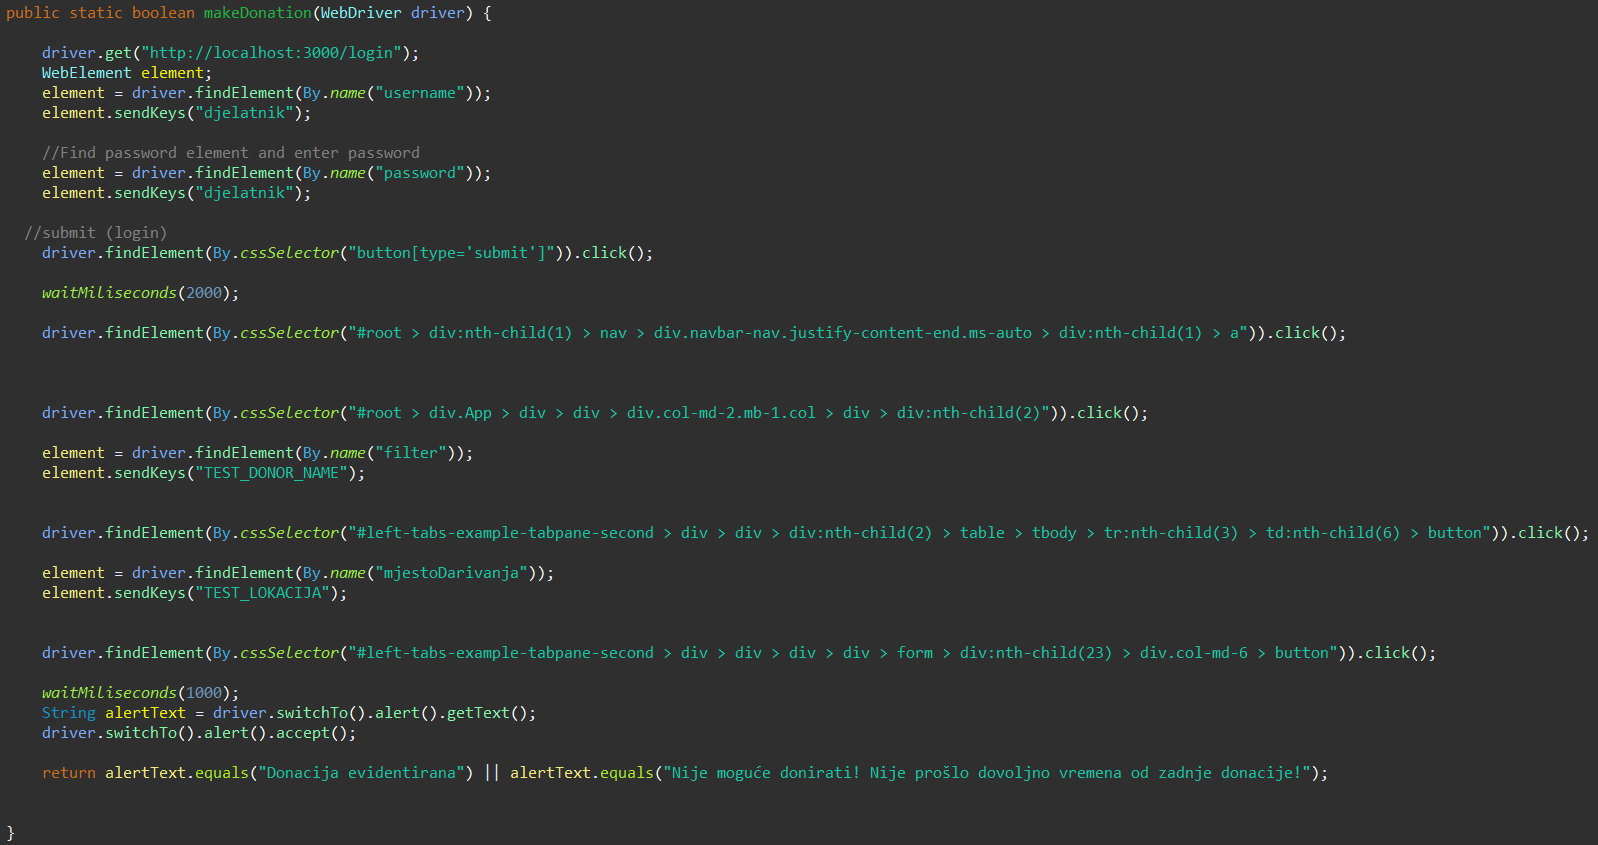
\includegraphics[width=\textwidth, scale=0.5]{slike/selenium4}
	\caption{Selenium test4}
\end{figure}
\eject
Te sve testne funkcije iskoristimo za provođenje testova u glavnoj (main) funkciji:
\begin{figure}[H]
	\centering
	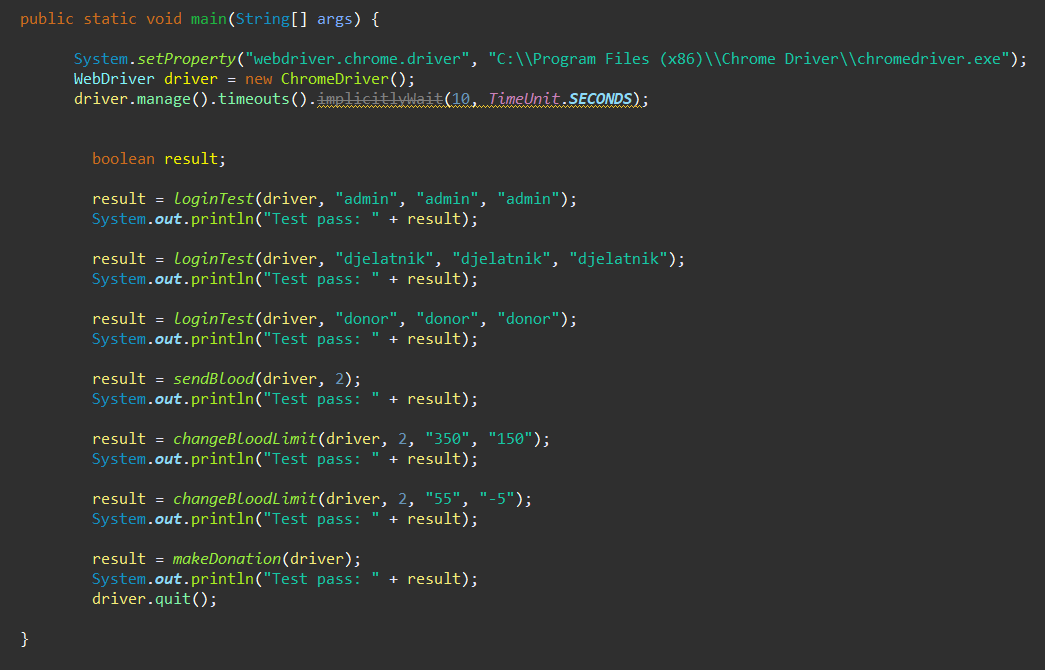
\includegraphics[width=\textwidth, scale=0.5]{slike/main}
	\caption{Funkcija main}
\end{figure}
\begin{figure}[H]
	\centering
	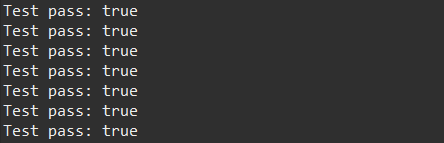
\includegraphics[width=\textwidth, scale=0.5]{slike/rezultat}
	\caption{Rezultat ispitivanja sustava}
\end{figure}
\eject
		\section{Dijagram razmještaja}
			
			Dijagrami razmještaja prikazuju topologiju sustava i odnos sklopovskih i program-
skih dijelova. Olakšavaju nam vizualizaciju razmještaja fizičkog dijela sustava i
sklopovlja. Sustav se sastoji od klijentskog i poslužiteljskog računala. Klijent na
svojem računalu preko web preglednika pristupa aplikaciji. Klijentsko računalo
komunicira s poslužiteljskim računalom preko HTTP veze. Na poslužiteljskom se
računalu nalaze web poslužitelj i poslužitelj baze podataka (PostgreSQL).

\begin{figure}[H]
	\centering
	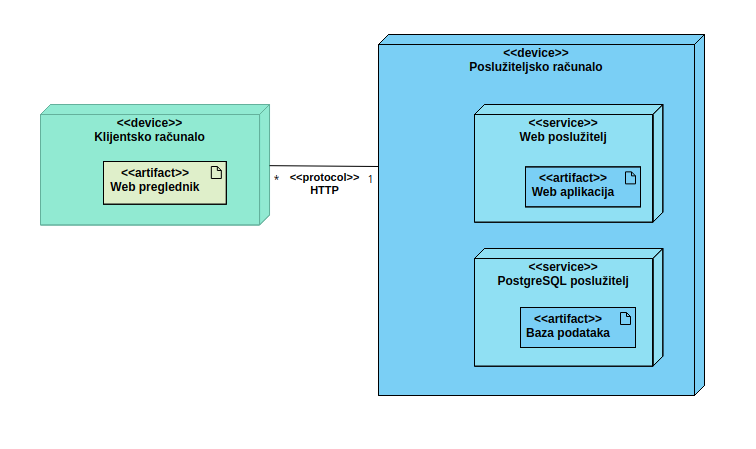
\includegraphics[width=\textwidth, scale=0.5]{dijagrami/dijagram_razmjestaja}
	\caption{Dijagram razmještaja}
	\label{fig:dijagram_razmještaja}
\end{figure}
\eject
	
			
		
		\section{Upute za puštanje u pogon}
		
		Ove upute vrijede te su rađene za Windows Server 2019 desktop experience operativni sustav. Slična (ili gotovo ista) procedura je i za ostale Windows, pa čak i Linux operativne sustave. Većina razlika je u samoj instalaciji potrebnih programskih paketa i runtime-a te postavljanje putanje, nakon čega je konfiguriranje aplikacije i njezino korištenje gotovo identično.
		
			\subsection{Instalacija poslužitelja baze podataka}
			Potrebno je preuzeti {PostgreSQL bazu podataka za Windows x86-64}\footnote{\url{https://www.enterprisedb.com/downloads/postgres-postgresql-downloads/}}. Preporuča se verzija 13.x. Prilikom instalacije preporuča se ostaviti sve (po defaultu) označene komponente za instalaciju, jer će kasnije biti potrebno inicijalno popuniti bazu pomoću pgAdmin4 alata. Odaberite šifru za korisnika postgres te port na kojem će baza podataka slušati zahtjeve. Prilikom završetka instalacije nije potrebno pokretati stack builder. Nakon instalacije (i prilikom svakog restarta servera), Windows automatski pokreće servis baze podataka, te je ona dostupna na prethodno specificiranom portu.
			
			\subsection{Instalacija Node.js runtime-a}
			Potrebno je preuzeti i instalirati {Node.js runtime}\footnote{\url{https://nodejs.org/en/download/}} koji će pokrenuti frontend dio aplikacije. Preporuča se trenutno dostupna LTS verzija (16.13.2 na dan pisanja). Prilikom instalacije potrebno je ostaviti sve (po defaultu) označene komponente za instalaciju, dok ponuđeni alat Chocolatey nije potrebno instalirati. Installer je automatski postavio PATH varijablu okruženja, te su \textit{npm} i \textit{node} naredbe postale globalno dostupne u cmd-u.
			\eject
			\subsection{Instalacija Jave}
			Potrebno je preuzeti i instalirati {JDK paket}\footnote{\url{https://www.oracle.com/java/technologies/downloads/jdk17-windows/}} koji će pokretati backend dio aplikacije.
			
			\begin{figure}[H]
			\centering
			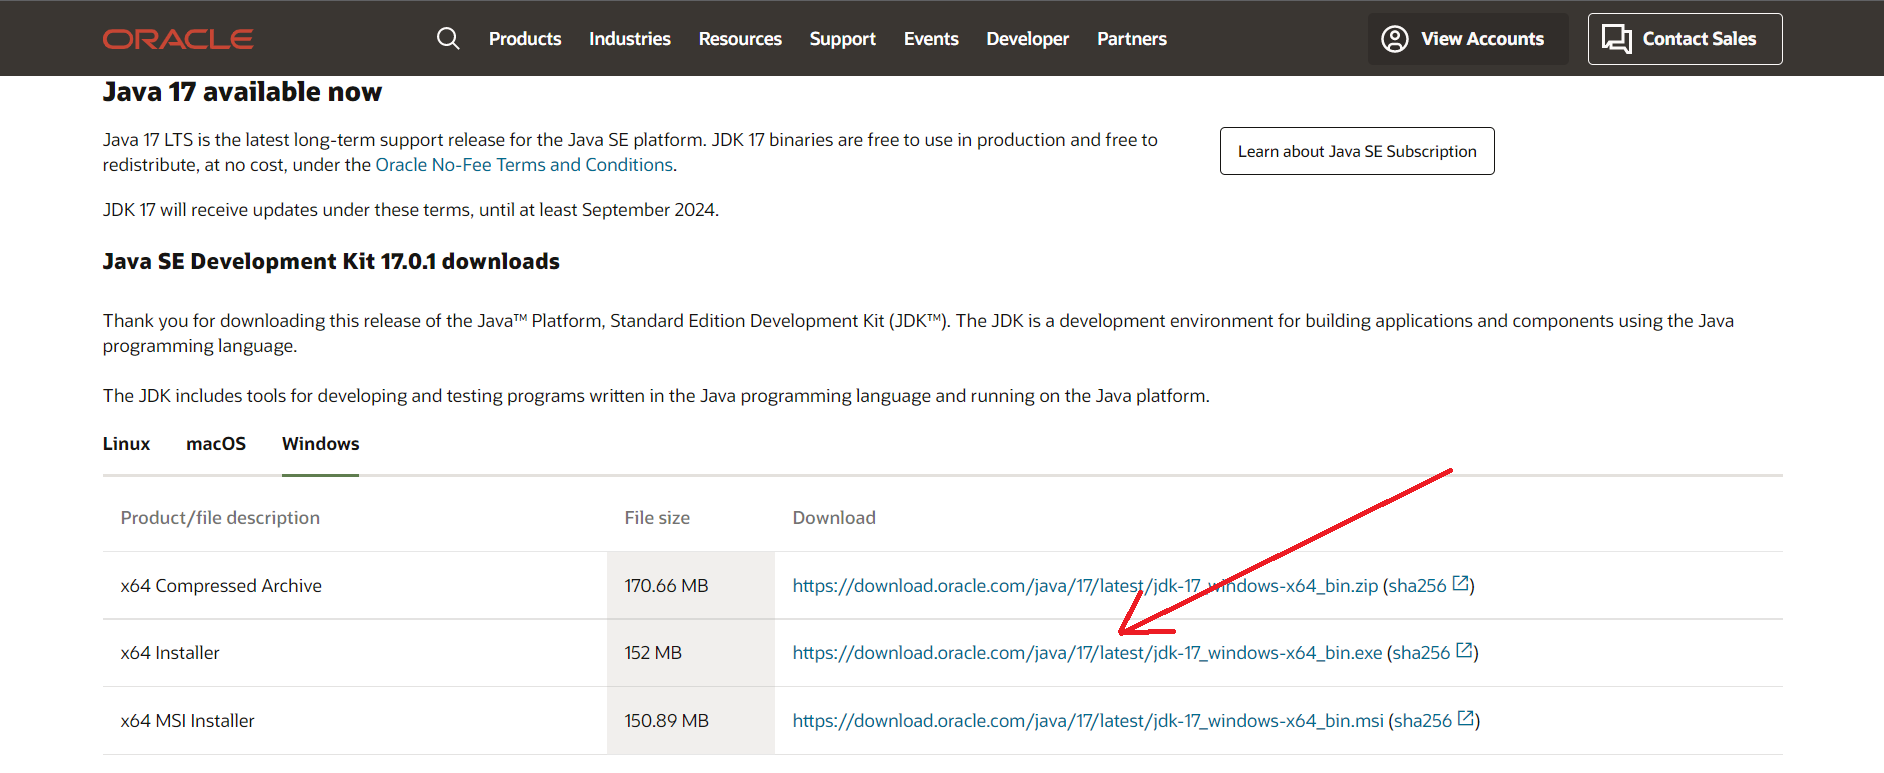
\includegraphics[width=\textwidth, scale=0.5]{slike/JDKdownload}
			\caption{Download JDK17 Installera}
			\label{fig:JDKdownload}
			\end{figure}

			Potrebna je trenutna 17.x.x verzija, no moguće je koristiti i neku od novijih verzija. Installer je automatski postavio PATH varijablu okruženja, te je \textit{java} naredba postala globalno dostupna u cmd-u.
			
			\subsection{Instalacija Maven alata i postavljanje PATH varijable okruženja}
			Potrebno je preuzeti {Maven alat}\footnote{\url{https://maven.apache.org/download.cgi/}} koji služi za kreiranje .jar datoteke iz izvornog koda koja sadrži cijelu backend aplikaciju sa web serverom. Preporuča se 3.8.4 verzija ili novija.
			
			\begin{figure}[H]
			\centering
			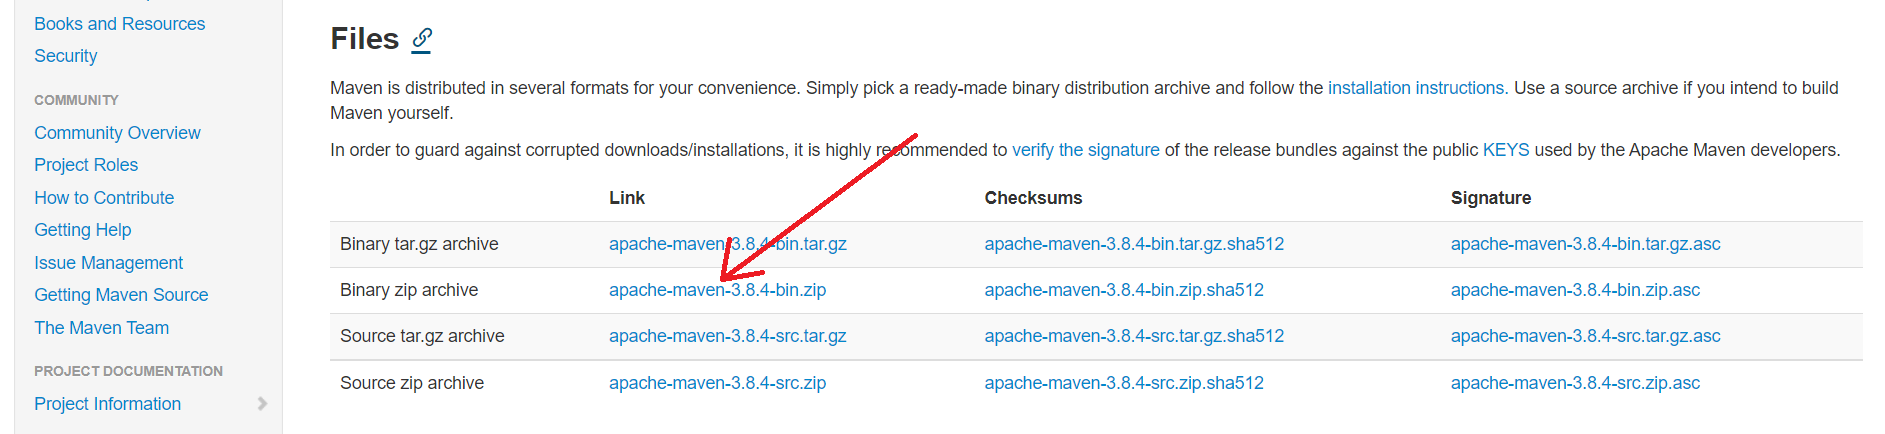
\includegraphics[width=\textwidth, scale=0.5]{slike/mavenDownload}
			\caption{Download Maven Binary-a}
			\label{fig:mavenDownload}
			\end{figure}
			
			\eject
			Nakon preuzimanja potrebno je raspakirati folder u proizvoljnu mapu (u ovom primjeru u \textit{C:/Program Files/apache-maven-3.8.4-bin}) te dodati \textit{bin} folder u PATH varijablu okruženja što se napravi na sljedeći način: 
			Pritiskom \textit{Windows} + \textit{R} tipki otvara se prozor u kojem treba napisati \textit{SystemPropertiesAdvanced} i pritisnuti Enter.
			
			\begin{figure}[H]
			\centering
			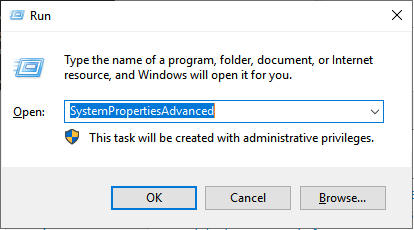
\includegraphics[width=\textwidth, scale=0.5]{slike/RunWindow}
			\caption{Prozor pokreni}
			\label{fig:RunWindow}
			\end{figure}
		
		\eject
			Nakon toga otvara se drugi prozor gdje treba pritisnuti gumb \textit{Environment Variables...}.
			
			\begin{figure}[H]
			\centering
			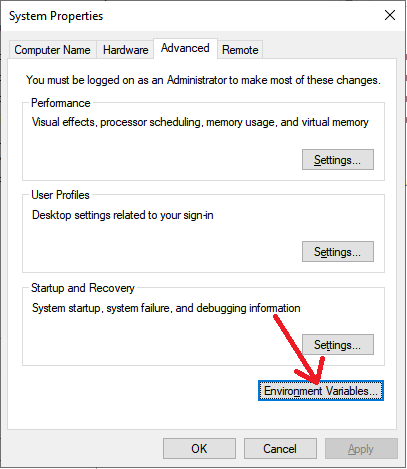
\includegraphics[width=\textwidth, scale=0.5]{slike/SystemPropertiesAdvanced}
			\caption{Prozor naprednih postavka sustava}
			\label{fig:SystemPropertiesAdvanced}
			\end{figure}
			
			\eject
			Time se otvara i treći prozor gdje treba locirati sistemsku \textit{Path} varijablu, označiti ju te pritisnuti gumb \textit{Edit...}
			
			\begin{figure}[H]
			\centering
			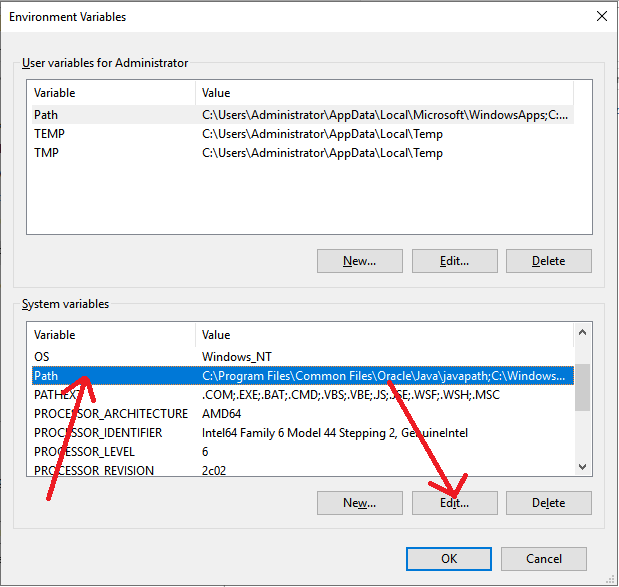
\includegraphics[width=\textwidth, scale=0.5]{slike/EnvironmentVariables}
			\caption{Prozor varijabli okruženja}
			\label{fig:EnvironmentVariables}
			\end{figure}
			
			\eject
			Nakon toga, u novootvorenom prozoru, pritiskom na tipku \textit{New} potrebno je napisati putanju do \textit{bin} foldera prethodno raspakiranog Maven alata. U ovom slučaju to je \textit{C/Program Files/apache-maven-3.8.4-bin/apache-maven-3.8.4/bin}.
			
			\begin{figure}[H]
			\centering
			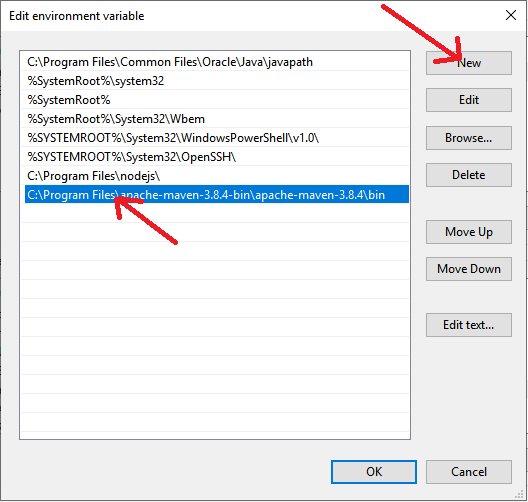
\includegraphics[width=\textwidth, scale=0.5]{slike/newPathInsert}
			\caption{Nova putanja u PATH varijabli okruženja}
			\label{fig:newPathInsert}
			\end{figure}
			
			\eject
			\subsection{Podešavanje i pokretanje backend dio aplikacije te inicijalno punjenje baze}
			Kako bi aplikacija ispravno radila, potrebno je postaviti parametre za povezivanje s bazom podataka te ispravnu IP adresu i port za aktivacijski link u datoteci \textit{application.properties} (koja se nalazi na putanji \textit{IzvorniKod/trueblood/src/main/resources}).
			
			\begin{figure}[H]
			\centering
			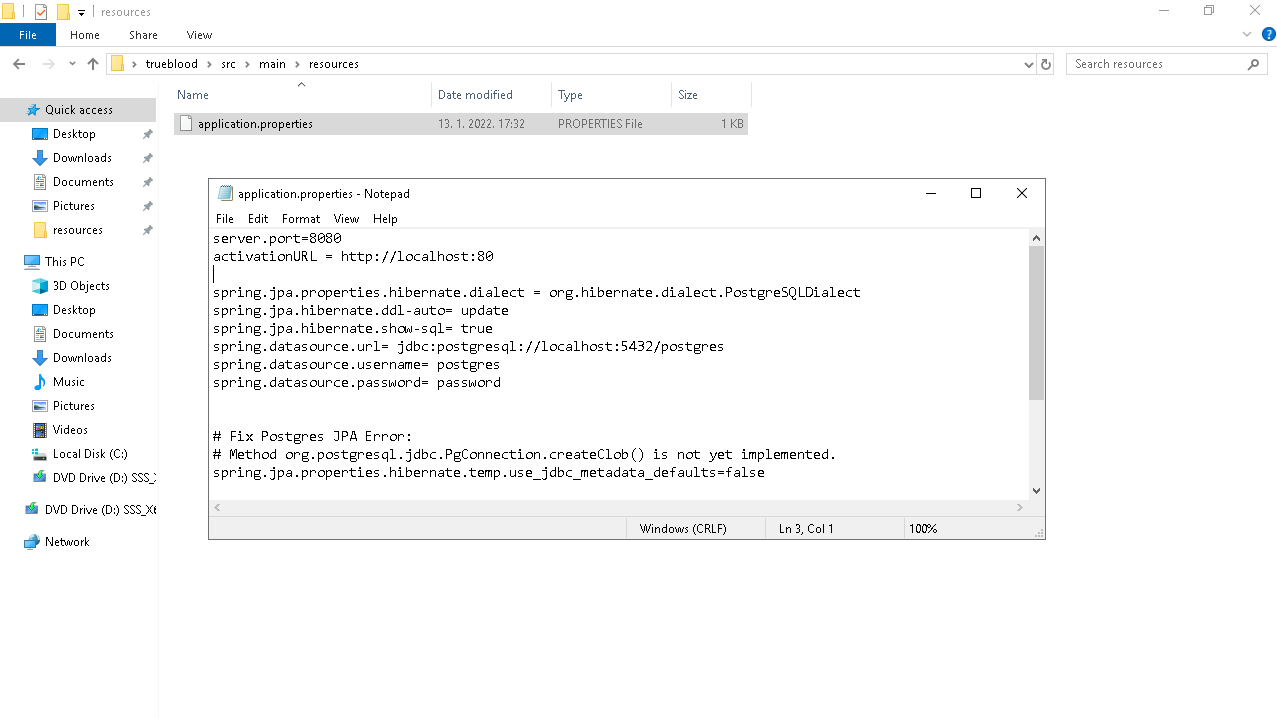
\includegraphics[width=\textwidth, scale=0.5]{slike/ApplicationProperties}
			\caption{application.properties datoteka}
			\label{fig:ApplicationProperties}
			\end{figure}
			
			Na samom vrhu nalazi se konfiguracijska linija \textit{server.port=8080} kojom se može promijeniti port backend servera (default je 8080).
			Ispod toga, nalazi se linija \textit{activationURL = http://localhost:80}. Ovdje je potrebno specificirati javnu IP adresu servera (ili DNS name tj. link ukoliko se koristi), te port frontend dijela aplikacije (ukoliko nije default 80). Jedan od načina kako se to može napraviti jest tako da se na serveru otvori stranica \textit{https://www.whatismyip.com/} te se kopira ispisana IP adresa na mjesto (activationURL = \textit{http://IPadresa:80})
			
			\eject
			
			\begin{figure}[H]
			\centering
			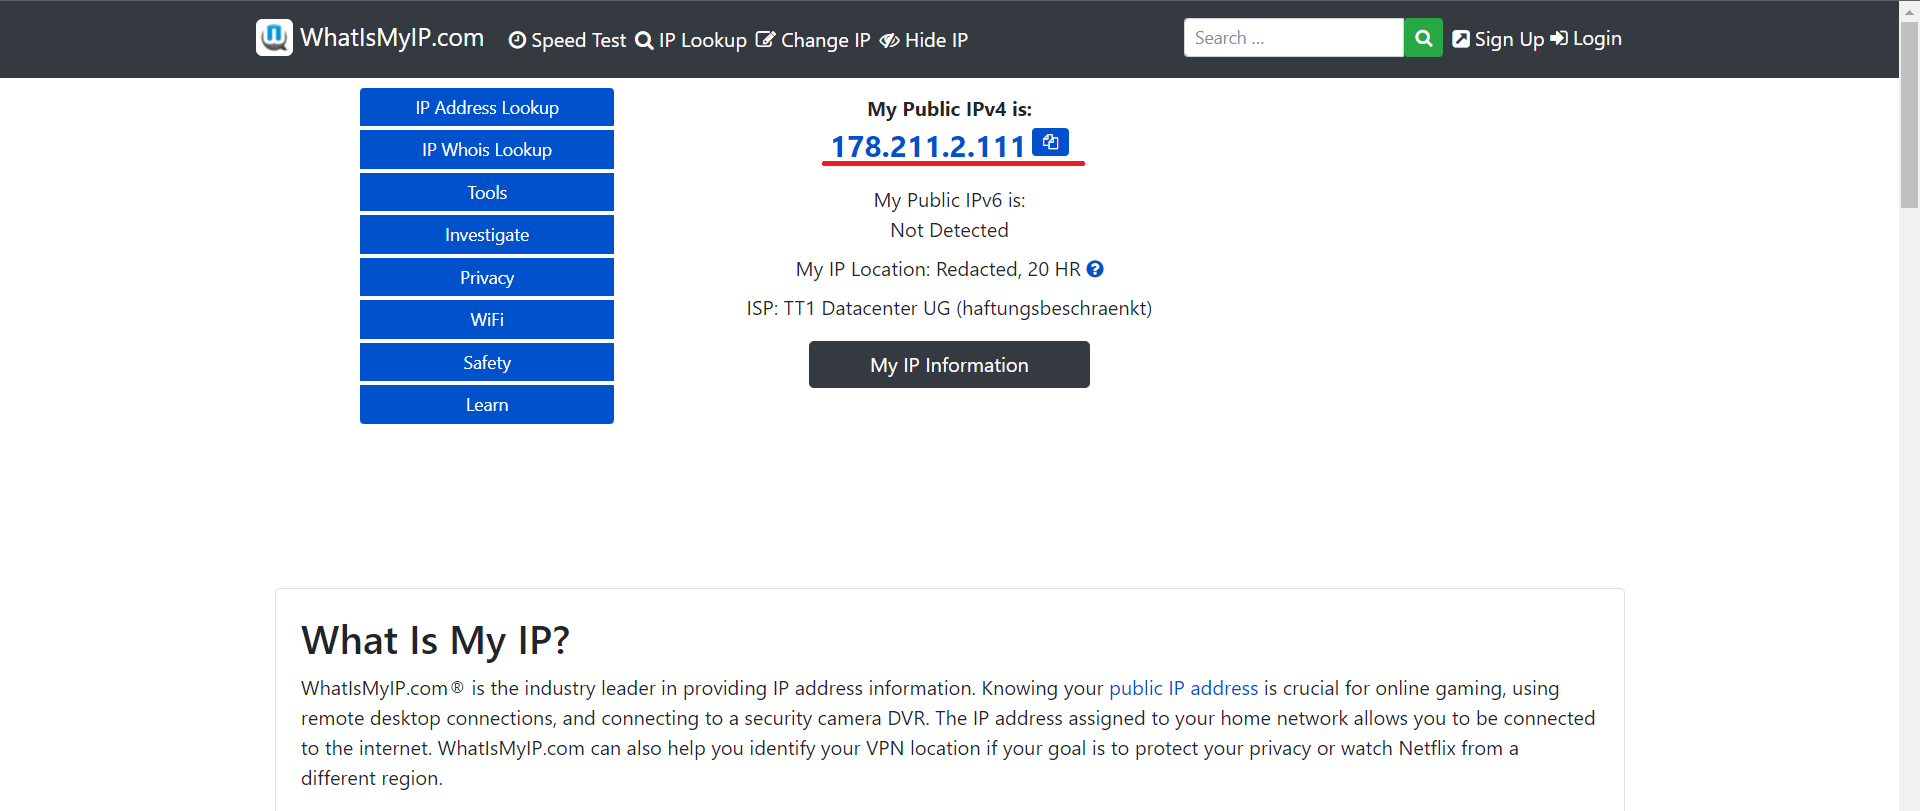
\includegraphics[width=\textwidth, scale=0.5]{slike/WhatIsMyIp}
			\caption{Kopiranje javne IPv4 adrese servera}
			\label{fig:WhatIsMyIp}
			\end{figure}

			Nadalje, ispod se nalaze 3 ključne linije za povezivanje s bazom:
			\begin{itemize}
				\item{\textit{spring.datasource.url= jdbc:postgresql://localhost:5432/postgres}}
				\item{\textit{spring.datasource.username= postgres}}
				\item{\textit{spring.datasource.password= password}}
			\end{itemize}			
			
			Na prvoj liniji je potrebno specificirati odabrani port prilikom instalacije 
			\textit{../localhost:portnumber/...}, te ime baze \textit{...5432/imebaze} ukoliko se ne koristi default baza.
			Na drugoj liniji specificira se ime korisnika kojeg aplikacija koristi za pristup bazi, te na trećoj liniji lozinka tog korisnika. Ukoliko se koristi default \textit{postgres} korisnik za koji je definirana lozinka prilikom instalacije, ovdje se upiše ta ista lozinka.\\
			
			Nakon modificiranja i spremanja konfiguracijske datoteke, potrebno je otvoriti cmd, pozicionirati se u trueBlood folder \textit{IzvorniKod/trueBlood} te izvršiti komandu \textit{mvn clean install -DskipTests} kojom će Maven alat preuzeti potrebne dependency-je te izraditi .jar datoteku spremnu za pokretanje.
			\eject
			
			\begin{figure}[H]
			\centering
			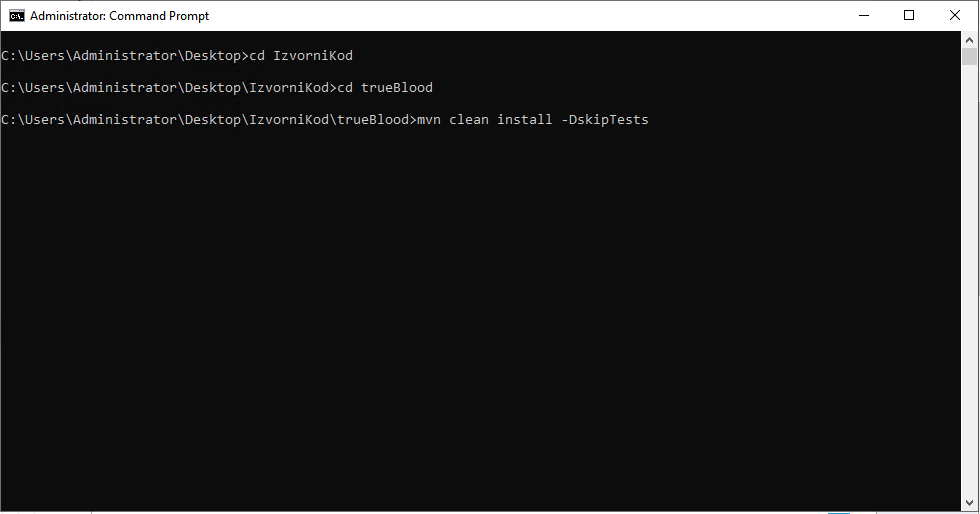
\includegraphics[width=\textwidth]{slike/CmdCommands}
			\caption{Pozicioniranje i izvršavanje komandi}
			\label{fig:CmdCommands}
			\end{figure}
				
			\begin{figure}[H]
			\centering
			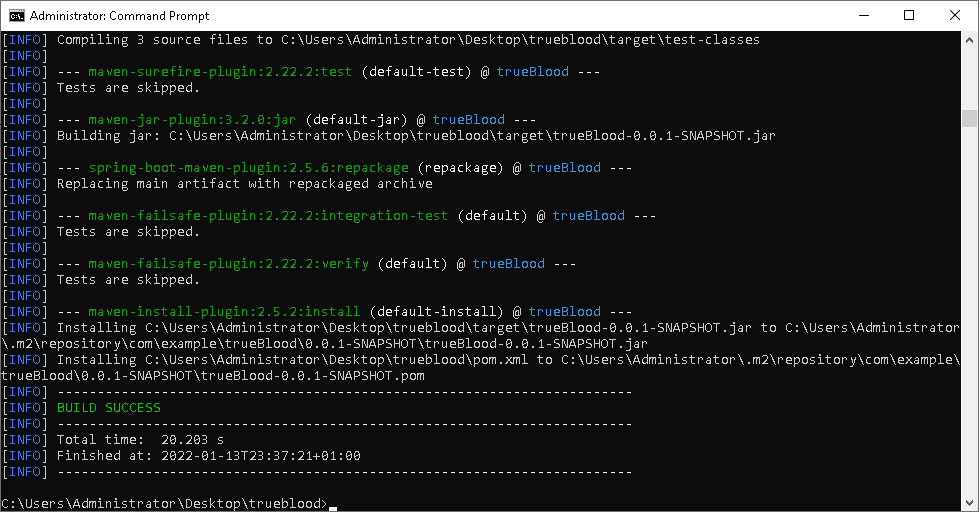
\includegraphics[width=\textwidth]{slike/cmdBuildFinished}
			\caption{Završni izlaz nakon uspješnog builda aplikacije}
			\label{fig:cmdBuildFinished}
			\end{figure}
			\eject
			Izrađena .jar datoteka (koja u sebi sadrži sve što je potrebno za njezino pokretanje, uključujući i Tomcat web server) nalazi se na putanji \textit{IzvorniKod/trueBlood/target} pod imenom \textit{trueBlood-0.0.1-SNAPSHOT}, te se sa cmd-om potrebno pozicionirati u navedeni folder i izvršiti komandu \textit{java -jar trueBlood-0.0.1-SNAPSHOT.jar} čime se pokreće backend dio aplikacije. Potrebno je ostaviti otvoren cmd prozor kako bi aplikacija radila.\\\\
			
			Aplikacija sama stvara tablice i strukturu podataka u schemu \textit{public} unutar baze specificirane u \textit{application.properties}. No za ispravan rad potrebno je još dodavanje statičkih redova na način da se otvori prije instalirana aplikacija PgAdmin, desnim klikom na korištenu bazu odabere se \textit{Query Tool}, te u tekstni prozor se kopira sadržaj datoteke \textit{puniteljBaze.sql} (koja se nalazi na putanji \textit{IzvorniKod/trueblood/puniteljBaze.sql}). Ovim početnim punjenjem baze podataka, definira se početni admin korisnički račun (username: \textit{admin}, password: \textit{admin}) pomoću kojeg je moguće daljnje upravljanje aplikacijom.
			
			\begin{figure}[H]
			\centering
			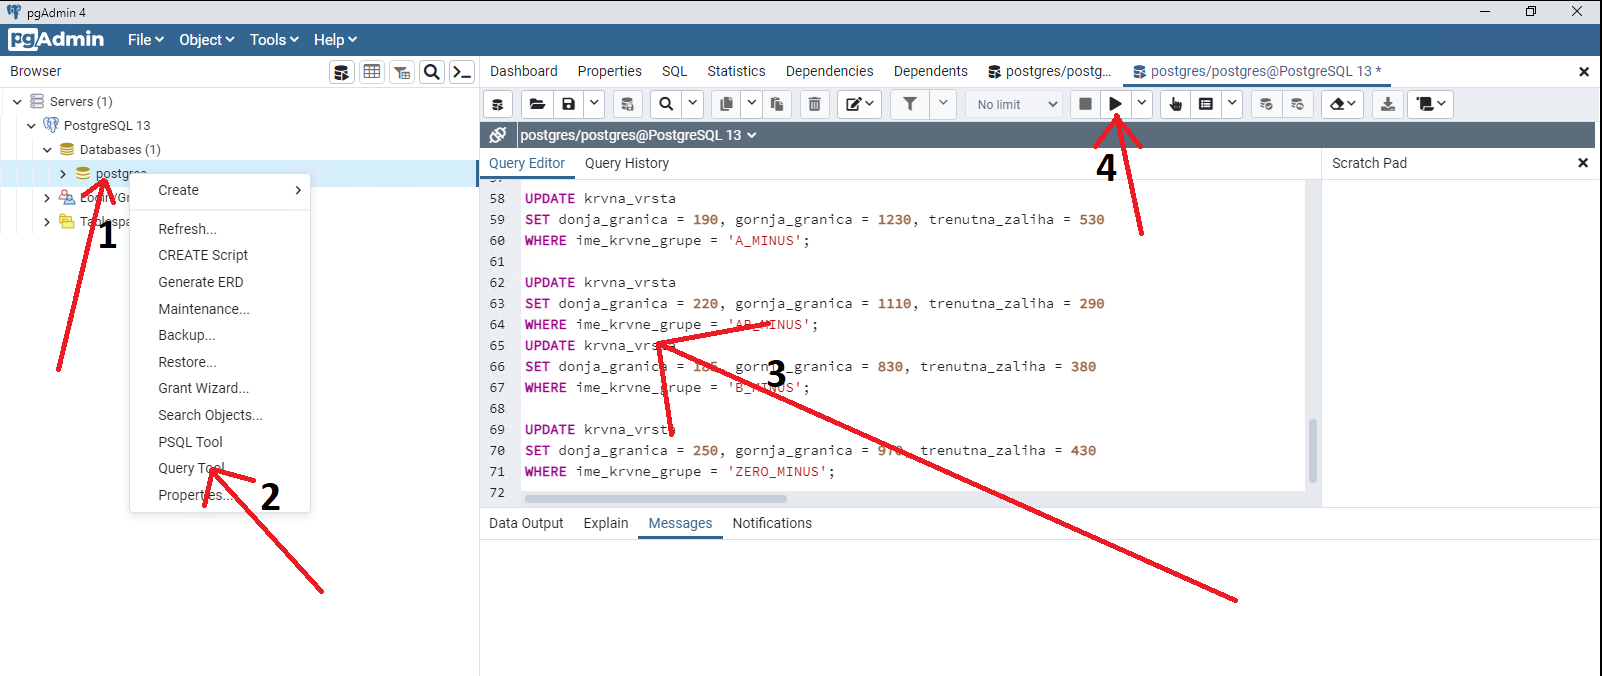
\includegraphics[width=\textwidth, scale=0.5]{slike/puniteljBaze}
			\caption{Punjenje baze statičkim podacima}
			\label{fig:puniteljBaze}
			\end{figure}
			\eject
			\subsection{Podešavanje i pokretanje frontend dijela aplikacije}
			Nakon uspješno pokrenutog backend dijela aplikacije, potrebno je još posložiti i pokrenuti i frontend dio aplikacije. Potrebno je javnu IP adresu servera i port backend dijela aplijacije (definiranog prije u \textit{application.properties}) upisati u datoteku \textit{Constants.js} koja se nalazi na putanji \textit{IzvorniKod/trueBlood/frontend/src/components} na liniji \textit{export const SPRINGURL = 'http://localhost:8080'}.
		
			\begin{figure}[H]
			\centering
			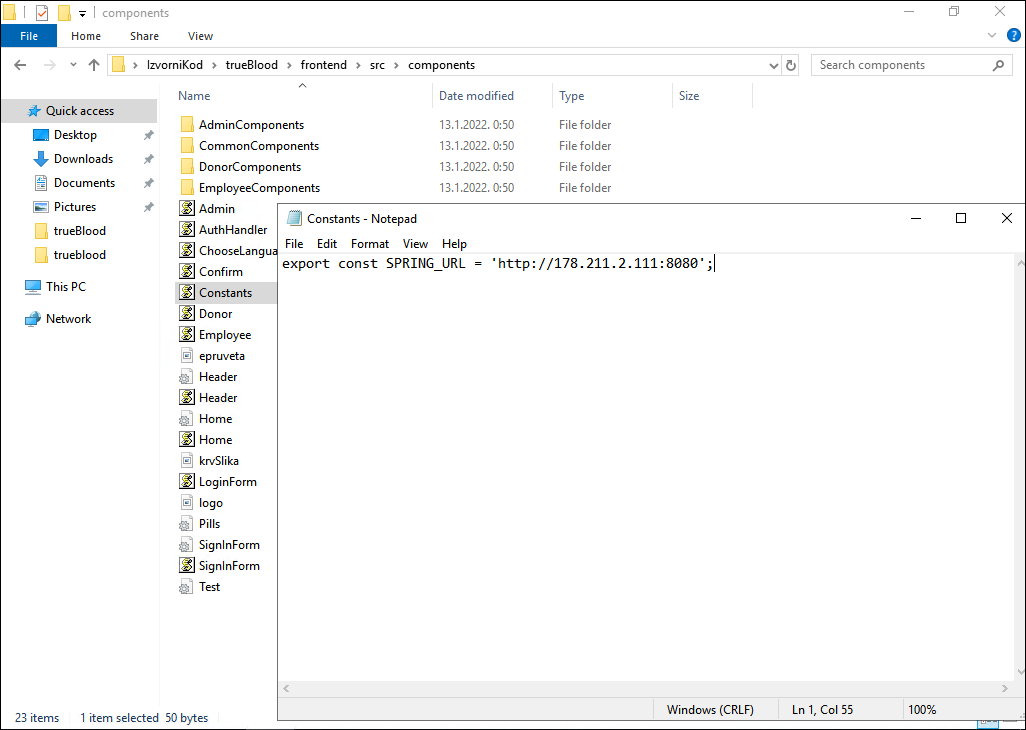
\includegraphics[width=\textwidth, scale=0.5]{slike/ConstantsJs}
			\caption{Constants.js datoteka}
			\label{fig:ConstantsJs}
			\end{figure}
			\eject
			Nakon modificiranja i spremanja datoteke Constants.js, potrebno je otvoriti novi cmd prozor, pozicionirati se u frontend folder (putanja \textit{IzvorniKod/trueBlood/frontend}) te izvršiti komandu \textit{npm install} kojom se instaliraju potrebni node moduli. Zatim komandu \textit{npm run build} kojom se kreira folder u kojem se nalaze izvršne datoteke spremne za korištenje u produkciji. Te datoteke mogu se upogoniti u bilo kojem proizvoljnom web serveru (poput microsoftovog IIS-a), no radi jednostavnosti, nakon izvršenja prethodne naredbe, naredbom \textit{npm install -g serve} dodatno se instalira \textit{serve} modul, koji koristi za posluživanje prije kreiranih datoteka. Napokon, naredbom \textit{serve -s build -l 80} pokreće se Node.js web server na portu 80, te je ovime kompletna aplikacija spremna za upotrebu.
			
			\subsection{Napomene}
			
			Ukoliko je uključen, potrebno je odabrane portove frontend i backend dijela aplikacije propustiti kroz firewall.\\\\
			Ukoliko nakon pokretanja backend ili frontend dijela aplikacije neki od njih izgledno ne radi, moguće da se slučajnim lijevim klika mišom na cmd prozor (koji ga pokreće taj dio aplikacije zamrznuo. Potrebno je na taj isti prozor pritisnuti desni klik miša, što će nastaviti rad zamrznutog dijela aplikacije. Preporuča se minimiziranje cmd prozora kako ne bi došlo do tog problema.
			
			
			\eject
	\chapter{Zaključak i budući rad}
		
		Naš zadatak bio je izraditi banku krvi koju bi primarno koristili donori i djelatnici banke.
	
	Ideja banke krvi i upravljanje količinama krvi je sveprisutna u svijetu, a dostupna je i na mrežnim stranicama \underline{HZTM}\footnote{\url{http://hztm.hr/hr/content/22/zalihe-krvi/831/zalihe-krvi}}.
\\\\
	Projekt smo proveli u tri faze:
	\begin{enumerate}
		\item početna razrada funkcionalnih i nefunkcionalnih zahtjeva
		\item implementacija zahtjeva i daljnje razrađivanje
		\item testiranje i završno dokumentiranje
	\end{enumerate} 

	Na početku prve faze upoznavali smo ideju aplikacije, razrađivali smo funkcionalne zahtjeve i dogovarali se što sve aplikacija može i treba raditi. U prvoj fazi smo se također počeli upoznavati s tehnologijama koje smo koristili. Ni jedan od članova tima nije bio u potpunosti upoznat s tim tehnologijama. Naučili smo da u stvarnosti, prije izrade samog projekta, potrebno je naučiti kako učiti alate, a zatim i naučiti sam alat.
	
	U drugoj fazi projekta krenuli smo sa implementacijom, što je na početku teklo jako sporo jer još nismo bili upoznati s alatima, no kako je vrijeme prolazilo tako smo postajali bolji i implementirali smo zahtjeve sve brže. Također, u ovoj fazi uvidjeli smo propuste u definicijama funkcionalnih i nefunkcionalnih zahtjeva, pa smo naučili biti precizniji u svojim definicijama i uzimati više slučajeva u obzir. 
	
	U trećoj, odnosno posljednjoj fazi, nakon implementacije programskog rješenja, dovršili smo dokumentaciju projekta. Ovaj korak nam je dodatno pomogao u shvaćanju obujma našeg projekta, i ukazao nam na arhitekturalne probleme koje nismo predvidjeli. Također, testiranjem smo ustanovili da sustav ima par grešaka.
	
	Članovi tima su prije projekta bili upoznati s Javom i NodeJS-om, pa bi odabirom tih tehnologija umjesto Reacta pomogao pri ubrzanju razvoja aplikacije. 
	
	Naučili smo važnost koordinacije i komunikacije među članovima tima. Nekad članovi nisu bili dobro koordinirani pa bi jedni implementirali funkcionalnost na ovaj, a drugi na onaj način. Naučili smo meke vještine povezane s projektima općenito, kao što je korištenje alata \texttt{git}, pisanje značajnih commit poruka, korištenje GitLab-a, te poštivanje unaprijed definiranih obrazaca programiranja. 
	
	Najviše od svega, naučili smo značenje vremenske koordiniranosti u grupnom radu. Projekti poput ovoga vremenski su zahtjevni i ponekad se može dogoditi da jedan modul programskog rješenja kasni za drugim, pa drugi ne može nastaviti svoj razvoj. U ovakvim slučajevima, iznimno je važno vremenski se uskladiti unutar tima kako bi se takve neučinkovitosti izbjegle. 
	
	Od definiranih funkcionalnih zahtjeva uspjeli smo implementirati sve koju su bili predstavljeni zadatkom.
	
	U budućnosti bismo mogli ažurirati aplikaciju i nadodati neke nove stvari. Primjerice, mogli bi donirati ljudi iz nekih drugih zemalja, pa bi aplikaciju preveli na engleski jezik. Također dodali bismo da djelatnik i administrator mogu biti ujedno i donori, što trenutno nije slučaj.

	Zaključno, zahvaljujući iskustvima i znanjima koja smo stekli na ovom projektu, kad bismo krenuli iz početka, napravili bismo mnogo bolji projekt mnogo brže.
	\eject 


	\chapter{Popis literature}
		\addcontentsline{toc}{chapter}{Popis literature}
	 	
 		\textbf{\textit{Kontinuirano osvježavanje}}
	
		\textit{Popisati sve reference i literaturu koja je pomogla pri ostvarivanju projekta.}
		
		
		\begin{enumerate}
			
			
			\item  Programsko inženjerstvo, FER ZEMRIS, \url{http://www.fer.hr/predmet/proinz}
			
			\item  I. Sommerville, "Software engineering", 8th ed, Addison Wesley, 2007.
			
			\item  T.C.Lethbridge, R.Langaniere, "Object-Oriented Software Engineering", 2nd ed. McGraw-Hill, 2005.
			
			\item  I. Marsic, Software engineering book``, Department of Electrical and Computer Engineering, Rutgers University, \url{http://www.ece.rutgers.edu/~marsic/books/SE}
			
			\item  The Unified Modeling Language, \url{https://www.uml-diagrams.org/}
			
			\item  Astah Community, \url{http://astah.net/editions/uml-new}
		\end{enumerate}
		
		 
	
	
	\begingroup
	\renewcommand*\listfigurename{Indeks slika i dijagrama}
	%\renewcommand*\listtablename{Indeks tablica}
	%\let\clearpage\relax
	\listoffigures
	%\vspace{10mm}
	%\listoftables
	\endgroup
	\addcontentsline{toc}{chapter}{Indeks slika i dijagrama}


	
	\eject 
		
	\chapter*{Dodatak: Prikaz aktivnosti grupe}
		\addcontentsline{toc}{chapter}{Dodatak: Prikaz aktivnosti grupe}
		
		\section*{Dnevnik sastajanja}
		
		
		\begin{packed_enum}
			\item  sastanak
			
			\item[] \begin{packed_item}
				\item Datum: 14. listopada 2021.
				\item Prisustvovali: Svi
				\item Teme sastanka:
				\begin{packed_item}
					\item  inicijalni dogovor s CROZ djelatnicima
				\end{packed_item}
			\end{packed_item}
			
			\item  sastanak
			\item[] \begin{packed_item}
				\item Datum: 21. listopada 2021.
				\item Prisustvovali: Svi
				\item Teme sastanka:
				\begin{packed_item}
					\item  dogovor oko podjele zadataka
					\item  podijeljeni zadaci iz dokumentacije na sedmero ljudi
				\end{packed_item}
			\end{packed_item}
			\item  sastanak
			\item[] \begin{packed_item}
				\item Datum: 28. listopada 2021.
				\item Prisustvovali: Jurinić, Kerman
				\item Teme sastanka:
				\begin{packed_item}
					\item  pripremljeni obrasci uporabe
					\item  podjela oko crtanja i opisivanja dijagrama
				\end{packed_item}
			\end{packed_item}
			\item  sastanak
			\item[] \begin{packed_item}
				\item Datum: 05. studenoga 2021.
				\item Prisustvovali: Jurinić, Hudiček, Vugrinec, Šlezak, Kerman
				\item Teme sastanka:
				\begin{packed_item}
					\item  klijentski dio aplikacije
					\item  dogovor oko poslužitelja
				\end{packed_item}
			\end{packed_item}
\eject
			\item  sastanak
			\item[] \begin{packed_item}
				\item Datum: 11. studenoga 2021.
				\item Prisustvovali: Jurinić, Hudiček, Vugrinec, Šlezak, Okreša, Kerman
				\item Teme sastanka:
				\begin{packed_item}
					\item  poslužiteljski dio aplikacije, dogovor oko dizajna baze podataka
				\end{packed_item}
			\end{packed_item}
			
			\item  sastanak
			\item[] \begin{packed_item}
				\item Datum: 12. studenoga 2021.
				\item Prisustvovali: Kerman
				\item Teme sastanka:
				\begin{packed_item}
					\item  konzultacije s asistentom i demosom oko obrazaca uporabe i baze podataka
				\end{packed_item}
			\end{packed_item}
			
			\item  sastanak
			\item[] \begin{packed_item}
				\item Datum: 17. studenoga 2021.
				\item Prisustvovali: svi
				\item Teme sastanka:
				\begin{packed_item}
					\item demonstracija aplikacije asistentu i demosu
				\end{packed_item}
			\end{packed_item}
			
			\item  sastanak
			\item[] \begin{packed_item}
				\item Datum: 9. prosinca 2021.
				\item Prisustvovali: svi
				\item Teme sastanka:
				\begin{packed_item}
					\item dogovor oko daljnjih aktivnosti
				\end{packed_item}
			\end{packed_item}
			
			\item  sastanak
			\item[] \begin{packed_item}
				\item Datum: 22. prosinca 2021.
				\item Prisustvovali: svi
				\item Teme sastanka:
				\begin{packed_item}
					\item demonstracija alfa inačice aplikacije asistentu i demosu
				\end{packed_item}
			\end{packed_item}
			
			%
			
		\end{packed_enum}
		
		\eject
		\section*{Tablica aktivnosti}
		
		
			
			 \textit{Napomena: Doprinose u aktivnostima treba navesti u satima po članovima grupe po aktivnosti.}

			\begin{longtblr}[
					label=none,
				]{
					vlines,hlines,
					width = \textwidth,
					colspec={X[7, l]X[1, c]X[1, c]X[1, c]X[1, c]X[1, c]X[1, c]X[1, c]}, 
					vline{1} = {1}{text=\clap{}},
					hline{1} = {1}{text=\clap{}},
					rowhead = 1,
				} 
				\multicolumn{1}{c|}{} & \multicolumn{1}{c|}{\rotatebox{90}{\textbf{David Kerman}}} & \multicolumn{1}{c|}{\rotatebox{90}{\textbf{Ivan Jurinić}}} &	\multicolumn{1}{c|}{\rotatebox{90}{\textbf{Matija Vugrinec}}} & \multicolumn{1}{c|}{\rotatebox{90}{\textbf{Jakov Šlezak}}} &	\multicolumn{1}{c|}{\rotatebox{90}{\textbf{Matej Hudiček}}} & \multicolumn{1}{c|}{\rotatebox{90}{\textbf{Marko Okreša}}} &	\multicolumn{1}{c|}{\rotatebox{90}{\textbf{Josip Pardon}}} \\  
				Upravljanje projektom 		& 10 &  &  &  &  &  & \\ 
				Opis projektnog zadatka 	&  &  &  & 4 &  &  & \\ 
				
				Funkcionalni zahtjevi       & 2 & 2 &  &  &  &  &  \\ 
				Opis pojedinih obrazaca 	& 6 & 6 &  &  &  &  &  \\ 
				Dijagram obrazaca 			& 4 & 2 &  &  &  &  &  \\ 
				Sekvencijski dijagrami 		&  &  &  &  & 4 &  &  \\ 
				Opis ostalih zahtjeva 		&  &  &  &  &  & 2 &  \\ 

				Arhitektura i dizajn sustava	 & 5 &  &  &  &  &  &  \\ 
				Baza podataka				&  &  & 10 &  &  &  &   \\ 
				Dijagram razreda 			& 3 &  &  &  & 5 &  & 6  \\ 
				Dijagram stanja				& 2 &  &  &  &  &  &  \\ 
				Dijagram aktivnosti 		& 3 &  &  &  &  &  &  \\ 
				Dijagram komponenti			& 1 &  &  &  &  &  &  \\ 
				Korištene tehnologije i alati 		& 2 &  &  &  &  &  &  \\ 
				Ispitivanje programskog rješenja 	& 5 &  &  &  &  &  & 5 \\ 
				Dijagram razmještaja			& 1 &  &  &  &  &  &  \\ 
				Upute za puštanje u pogon 		&  &  &  &  &  &  & 6 \\  
				Dnevnik sastajanja 			& 1 &  &  &  &  &  &  \\ 
				Zaključak i budući rad 		& 1 &  &  &  &  &  &  \\  
				Popis literature 			& 1 &  &  &  &  &  &  \\  
				&  &  &  &  &  &  &  \\ \hline 
				frontend 			&  & 20 &  &  & 45 &  & 30 \\ 
				backend 				& 40 &  & 40 & 45 &  & 30 &  \\  
				baza podataka		&  &  & 5 &  &  &  & \\  
				
			\end{longtblr}
					
					
		\eject
		\section*{Dijagrami pregleda promjena}
		
		
		    \begin{figure}[H]
			\centering
			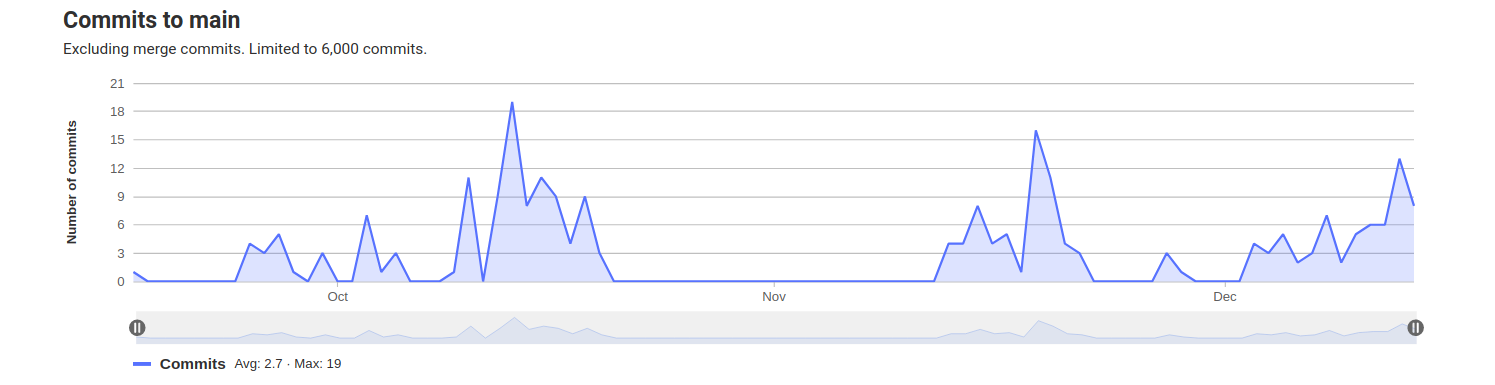
\includegraphics[width=\textwidth, scale=0.5]{dijagrami/dijagram_promjena1.png}
			\caption{Aktivnosti na main grani}
			\end{figure}
			
			
			 \begin{figure}[H]
			\centering
			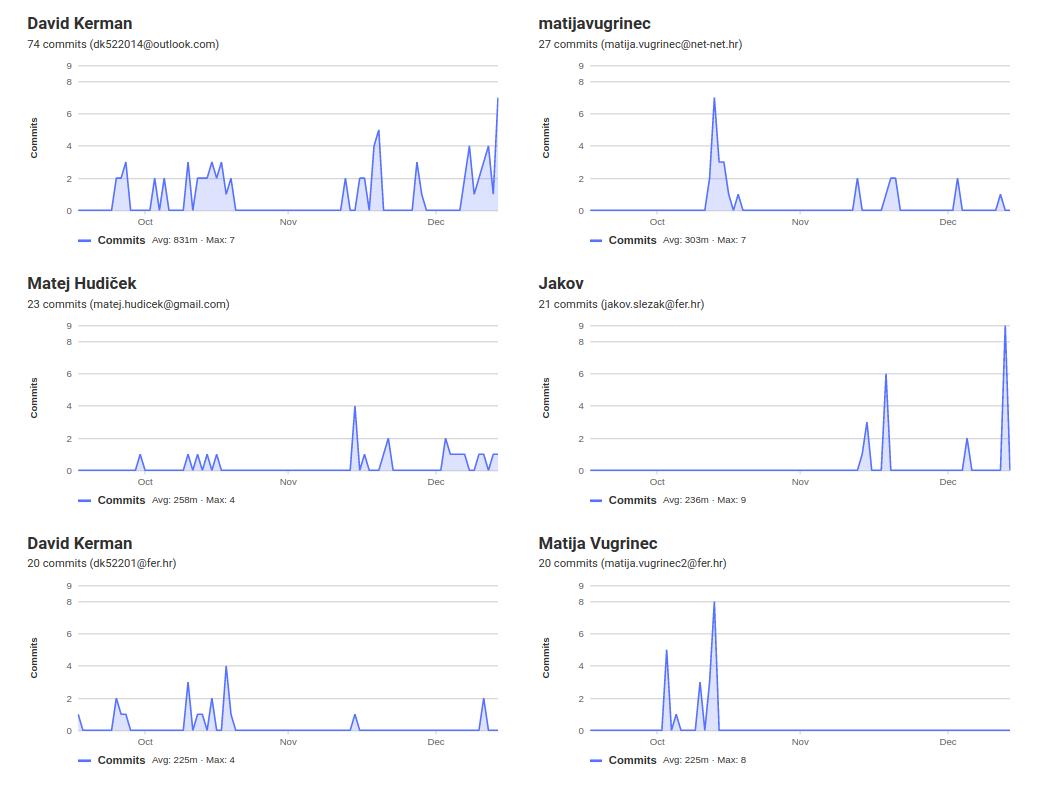
\includegraphics[width=\textwidth, scale=0.5]{dijagrami/dijagram_promjena2.png}
			\caption{Aktivnosti članova 1}
			\end{figure}
			
		    \eject
			 \begin{figure}[H]
			\centering
			\includegraphics[width=\textwidth, scale=0.5]{dijagrami/dijagram_promjena3.png}
			\caption{Aktivnosti članova 2}
			\end{figure}
		
	


\end{document} %naredbe i tekst nakon ove naredbe ne ulaze u izgrađen dokument 


